\chapter{Manual de usuario}\label{cap:manual_usuario}

\section{Introducción}

Sevillaneando es una aplicación móvil orientada al descubrimiento de eventos culturales y de ocio en Sevilla, con especial interés en dar visibilidad a propuestas emergentes o menos conocidas. Su finalidad no es únicamente mostrar un catálogo de actividades, sino ofrecer al usuario una experiencia completa de exploración, interacción y personalización a partir de sus intereses, su ubicación y su comportamiento dentro de la plataforma.

La aplicación permite consultar eventos, filtrarlos, localizarlos sobre el mapa, guardar aquellos que resulten de interés, apuntarse a ellos, compartirlos, valorarlos y participar en espacios de comunicación asociados. Además, incorpora funcionalidades avanzadas, como recomendaciones personalizadas y generación de rutas, que ayudan al usuario a descubrir nuevas actividades ajustadas a sus preferencias y a planificar mejor su asistencia.

Desde el punto de vista de uso, el sistema contempla distintos perfiles. El rol de usuario permite crear actividades. Por su parte, los roles de moderador y administrador cubren necesidades de supervisión y gestión interna de la aplicación.

El objetivo de este manual es guiar al usuario en el uso de la aplicación, describiendo sus principales entidades, requisitos de uso y flujos de interacción más relevantes. A lo largo del documento se explica cómo utilizar las distintas funcionalidades del sistema de manera progresiva, de forma que cualquier persona pueda comprender el funcionamiento general de la aplicación y aprovechar todas sus posibilidades.

\section{Definición de entidades y funcionalidades}

\begin{tcolorbox}[title=\textbf{Evento}]
El evento es la entidad principal del sistema y representa cada actividad cultural o de ocio disponible en la aplicación. Cada evento dispone de información descriptiva y funcional suficiente para que el usuario pueda decidir si le interesa asistir, guardarlo para más adelante o interactuar con él.

\vspace{0.4em}
\textbf{Funcionalidades}
\begin{itemize}[leftmargin=1.5em]
\item Creación de eventos públicos y privados.
\item Edición de la información del evento, como fecha, ubicación, descripción o precio.
\item Inscripción de usuarios.
\item Apertura de la ubicación del evento en aplicaciones externas de mapas.
\item Guardado del evento para consultas posteriores.
\item Visualización de asistentes.
\item Valoración del evento.
\item Acceso al chat asociado al evento.
\item Compartición del evento mediante enlace.
\item Gestión de estados: activo, finalizado y en moderación.
\item Inclusión en distintos listados personalizados.
\end{itemize}
\end{tcolorbox}

\begin{tcolorbox}[title=\textbf{Mapa de eventos}]
El mapa de eventos permite representar visualmente la distribución geográfica de las actividades disponibles. Esta funcionalidad resulta especialmente útil para usuarios que desean localizar eventos cercanos o comparar rápidamente varias opciones en función de su ubicación.

\vspace{0.4em}
\textbf{Funcionalidades}
\begin{itemize}[leftmargin=1.5em]
\item Visualización de eventos sobre mapa interactivo.
\item Clasificación aproximada por distancia mediante colores (verde, amarillo y rojo).
\item Configuración del radio de búsqueda.
\item Acceso directo al detalle del evento.
\item Uso de la ubicación del usuario como referencia.
\end{itemize}
\end{tcolorbox}

\begin{tcolorbox}[title=\textbf{Recomendaciones}]
El sistema de recomendaciones tiene como propósito adaptar la experiencia de uso a cada usuario. Para ello, tiene en cuenta factores como los intereses del perfil, la cercanía, las interacciones previas y otra información relevante del comportamiento dentro de la aplicación.

\vspace{0.4em}
\textbf{Funcionalidades}
\begin{itemize}[leftmargin=1.5em]
\item Recomendación de eventos según intereses del perfil.
\item Aprendizaje basado en la interacción del usuario.
\item Influencia de proximidad, valoraciones (propias y media global), eventos guardados, eventos apuntados, eventos vistos y eventos compartidos.
\item Consideración de fechas y disponibilidad.
\item Generación de rutas recomendadas.
\end{itemize}
\end{tcolorbox}

\begin{tcolorbox}[title=\textbf{Perfil de usuario}]
El perfil recoge la información personal y las preferencias del usuario. Esta entidad resulta fundamental, ya que condiciona parte del comportamiento personalizado del sistema, especialmente en lo relativo a recomendaciones y funciones basadas en ubicación.

\vspace{0.4em}
\textbf{Funcionalidades}
\begin{itemize}[leftmargin=1.5em]
\item Edición de datos personales.
\item Configuración de ubicación.
\item Gestión de intereses (categorías preferidas).
\item Cambio de contraseña.
\item Eliminación de cuenta.
\end{itemize}
\end{tcolorbox}

\begin{tcolorbox}[title=\textbf{Rutas}]
Las rutas son agrupaciones de eventos organizadas para facilitar la planificación del usuario. Pueden responder tanto a una lógica automática de recomendación como a la creación manual por parte de los propios usuarios. Este es otro punto clave, ya que permite agrupar eventos relacionados de forma coherente y optimizada en función de factores como la ubicación, el horario y las preferencias del usuario. De este modo, no solo se facilita la planificación de la asistencia a múltiples eventos, sino que también se incrementa la visibilidad de eventos relevantes que podrían pasar desapercibidos de forma individual, mejorando así el descubrimiento de contenido y la eficiencia en la experiencia de uso.

\vspace{0.4em}
\textbf{Funcionalidades}
\begin{itemize}[leftmargin=1.5em]
\item Generación automática de rutas recomendadas.
\item Creación manual de rutas por usuarios.
\item Optimización por distancia y horarios.
\item Consulta y valoración de rutas creadas por otros usuarios.
\end{itemize}
\end{tcolorbox}

\begin{tcolorbox}[title=\textbf{Notificaciones}]
El sistema de notificaciones mantiene informado al usuario sobre sucesos relevantes ocurridos dentro de la aplicación. Gracias a este módulo, la plataforma puede comunicar cambios de estado, recordatorios, eventos cercanos y actividad social de forma proactiva.

\vspace{0.4em}
\textbf{Funcionalidades}
\begin{itemize}[leftmargin=1.5em]
\item Notificación de aprobación o rechazo de eventos.
\item Recordatorios previos a eventos apuntados.
\item Avisos sobre eventos cercanos según la ubicación.
\item Notificación de nuevos seguidores.
\end{itemize}
\end{tcolorbox}

\begin{tcolorbox}[title=\textbf{Mensajería}]
Sistema de comunicación entre usuarios. Este módulo resulta fundamental dentro de la aplicación, ya que facilita la interacción directa entre participantes de un mismo evento o usuarios con intereses comunes. Gracias a esta funcionalidad, se promueve la conexión social, permitiendo coordinar asistencia, resolver dudas y organizar encuentros previos o durante el evento. Además, contribuye a mejorar la experiencia del usuario al fomentar la colaboración, la planificación compartida y la creación de redes sociales dentro de la plataforma.

\vspace{0.4em}
\textbf{Funcionalidades}
\begin{itemize}[leftmargin=1.5em]
\item Chat asociado a eventos.
\item Mensajes privados.
\item Acceso desde asistentes o perfiles de usuario.
\item Envío de texto e imágenes.
\end{itemize}
\end{tcolorbox}

\begin{tcolorbox}[title=\textbf{Amistad}]
El módulo de amistad permite descubrir y mantener contacto con otros usuarios de la plataforma. Aunque se apoya técnicamente en relaciones de seguimiento, la interfaz lo presenta como una sección social desde la que se pueden buscar usuarios, consultar perfiles, seguir o dejar de seguir a otras personas, enviar mensajes privados y ver los eventos a los que asisten.

\vspace{0.4em}
\textbf{Funcionalidades}
\begin{itemize}[leftmargin=1.5em]
\item Búsqueda de usuarios.
\item Listado completo de seguidores en la pestaña \textit{Seguidores}.
\item Listado de usuarios seguidos en la pestaña \textit{Seguidos}.
\item Listado de amistades mutuas en la pestaña \textit{Amigos}, cuando dos usuarios se siguen entre sí.
\item Acceso a listas independientes de seguidores y seguidos desde los contadores del perfil público.
\item Acceso al perfil de otros usuarios, con opción de seguir, dejar de seguir, enviar mensaje y consultar eventos a los que asisten.
\end{itemize}
\end{tcolorbox}

\begin{tcolorbox}[title=\textbf{Administración}]
La administración cubre las funciones de gestión global de la plataforma reservadas al rol de administrador.

\vspace{0.4em}
\textbf{Funcionalidades}
\begin{itemize}[leftmargin=1.5em]
\item Consulta de estadísticas globales de usuarios y eventos.
\item Gestión de usuarios y roles.
\item Gestión de categorías.
\item Restablecimiento administrativo de eventos importados por scraping.
\end{itemize}
\end{tcolorbox}

\begin{tcolorbox}[title=\textbf{Moderación}]
La moderación se ocupa de supervisar los contenidos que deben ser validados antes de su publicación y de mantener la coherencia y fiabilidad de los eventos ya publicados.

\vspace{0.4em}
\textbf{Funcionalidades}
\begin{itemize}[leftmargin=1.5em]
\item Revisión de eventos pendientes de aprobación.
\item Edición previa a la publicación.
\item Aprobación o rechazo de eventos.
\item Edición y eliminación de cualquier evento público ya aprobado.
\end{itemize}
\end{tcolorbox}

\section{Requisitos técnicos}

Para utilizar correctamente la aplicación es necesario disponer de los siguientes elementos:

\begin{itemize}[leftmargin=1.5em]
\item Un dispositivo móvil compatible con iOS o Android.
\item Conexión a Internet, ya sea mediante WiFi o datos móviles.
\item Una cuenta de correo electrónico válida para el registro y recuperación de contraseña.
\item Permisos recomendados de acceso a cámara y galería, necesarios para funcionalidades de imagen.
\item Permisos de ubicación, recomendables para el uso del mapa y la recepción de notificaciones cercanas.
\end{itemize}

\section{Guía de uso de la aplicación}

Una vez definidas las entidades principales del sistema, en esta sección se describe el uso práctico de la aplicación desde la perspectiva del usuario. El objetivo no es únicamente enumerar pantallas, sino explicar cómo puede utilizarse la plataforma para cubrir necesidades reales, como descubrir eventos, organizar la asistencia, comunicarse con otros usuarios o gestionar actividades propias.

\clearpage

\subsection{Registro e inicio de sesión (para todos los roles)}

El primer paso para utilizar la aplicación consiste en crear una cuenta. Al abrir la aplicación por primera vez se muestra la pantalla de inicio de sesión, desde la que el usuario puede acceder al formulario de registro pulsando el enlace inferior que indica que aún no dispone de cuenta. En la pantalla de registro debe introducir su nombre completo, una dirección de correo electrónico válida y una contraseña. La contraseña debe escribirse dos veces, en el campo principal y en el campo de confirmación, para evitar errores; mediante el icono con forma de ojo situado a la derecha de cada campo puede mostrarse u ocultarse temporalmente lo escrito. La aplicación exige que la contraseña tenga al menos seis caracteres y que ambas coincidan.

Antes de poder completar el alta, el usuario debe marcar la casilla de aceptación de la política de privacidad situada bajo los campos de contraseña. El texto que la acompaña incluye un enlace remarcado que abre la política completa en una pantalla independiente, donde puede consultarse íntegramente antes de aceptar. Una vez marcada la casilla, basta con pulsar el botón principal para crear la cuenta. Si alguno de los datos es incorrecto, no se acepta la política o el correo ya está registrado, la pantalla muestra un mensaje de error explicativo bajo el formulario y permite corregir lo necesario sin perder lo escrito. Aunque la plataforma contempla distintos roles, el registro siempre crea una cuenta con rol de usuario; los roles de moderador y administrador son asignados manualmente por el administrador principal, al que puede contactarse a través del correo electrónico mostrado al final de la página de inicio.

Una vez creada la cuenta, el acceso posterior se realiza desde la pantalla de inicio de sesión introduciendo el correo y la contraseña. Bajo los campos aparece la casilla \textit{Mantener sesión iniciada}, que conviene marcar si se desea que el correo quede recordado en futuros accesos. Si el usuario no recuerda la contraseña, debe escribir su correo en el primer campo y pulsar el enlace \textit{¿Olvidaste tu contraseña?} situado bajo el botón de inicio de sesión; la aplicación envía entonces un mensaje al correo indicado con las instrucciones para restablecerla. Tras completar el cambio desde el correo, puede volver a la pantalla de inicio de sesión e introducir la nueva contraseña con normalidad.

\bigskip

\textbf{Aspectos a tener en cuenta:}
\begin{itemize}[leftmargin=1.5em]
\item El correo electrónico debe ser válido.
\item La contraseña debe recordarse o recuperarse mediante el correo asociado.
\item La aceptación de la política de privacidad es obligatoria para crear la cuenta.
\item El registro crea cuentas con rol de usuario.
\end{itemize}

\begin{figure}[H]
    \centering
    \begin{subfigure}{0.35\linewidth}
        \centering
        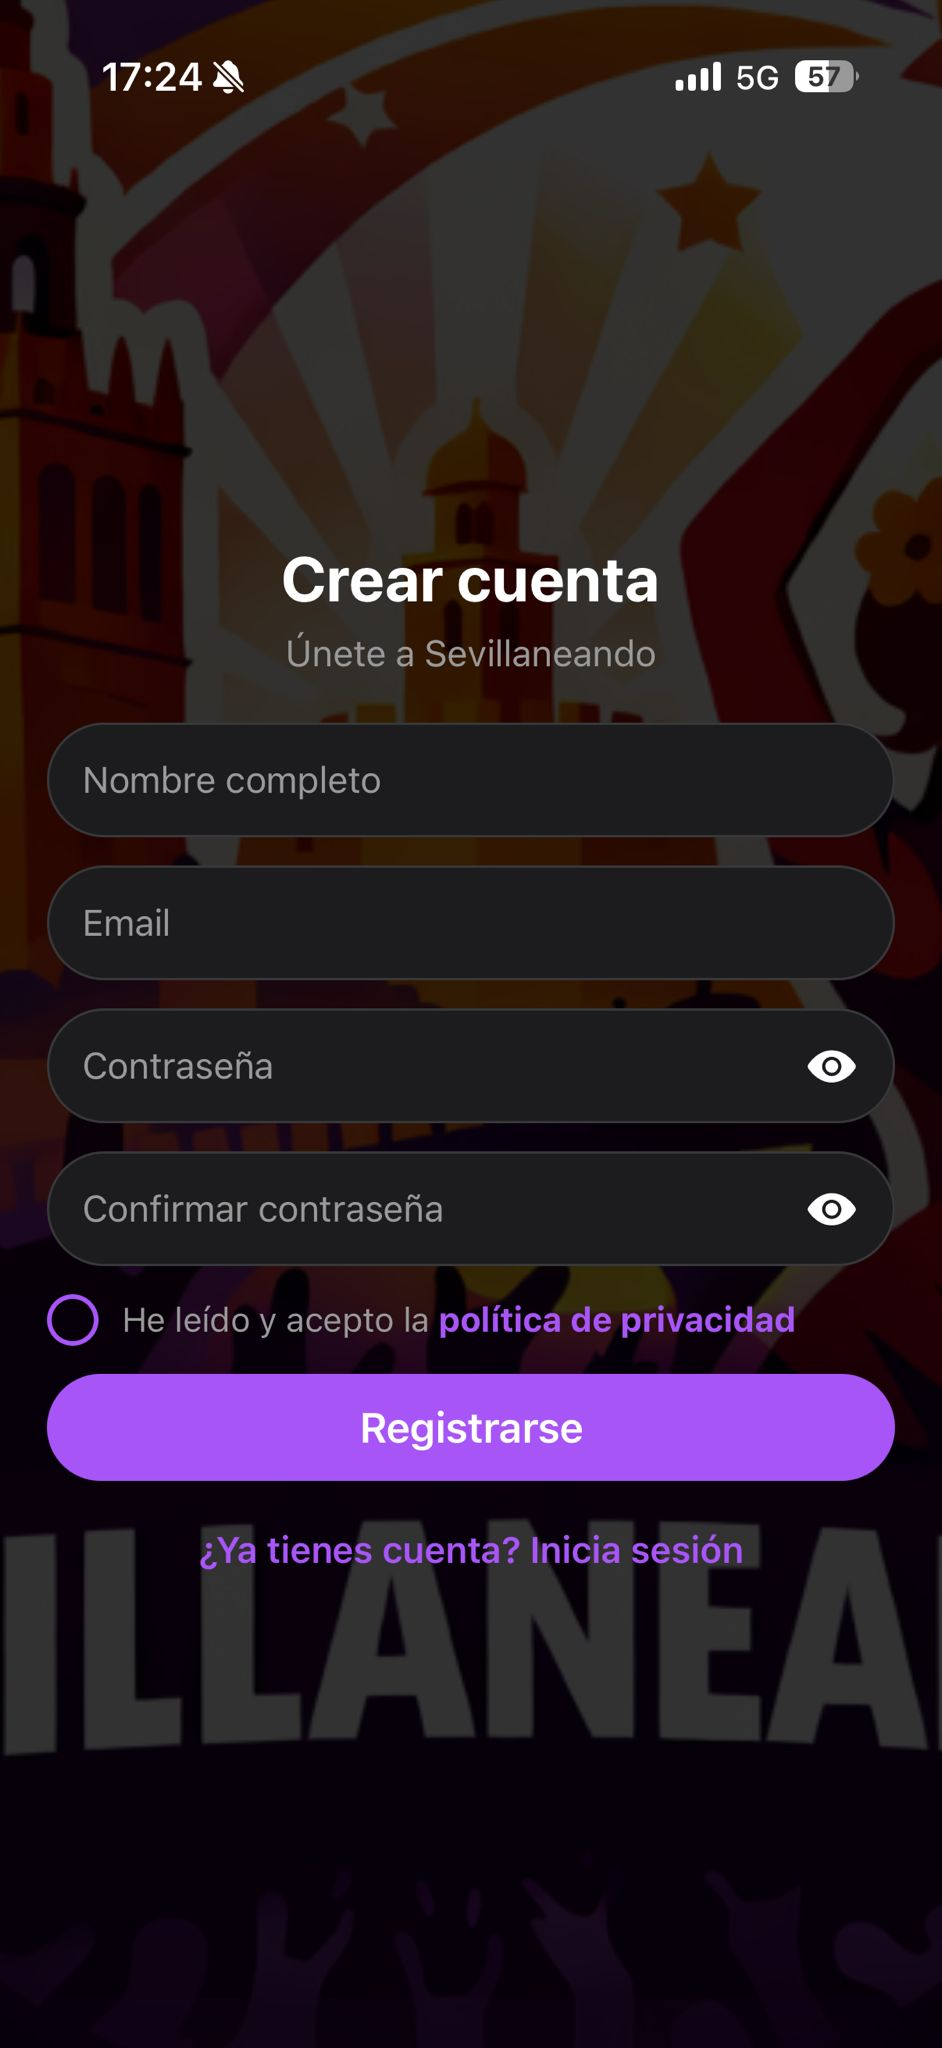
\includegraphics[width=\linewidth]{figures/paso1/crear_cuenta.png}
        \caption{Crear cuenta}
    \end{subfigure}
    \hspace{0.1\linewidth}
    \begin{subfigure}{0.35\linewidth}
        \centering
        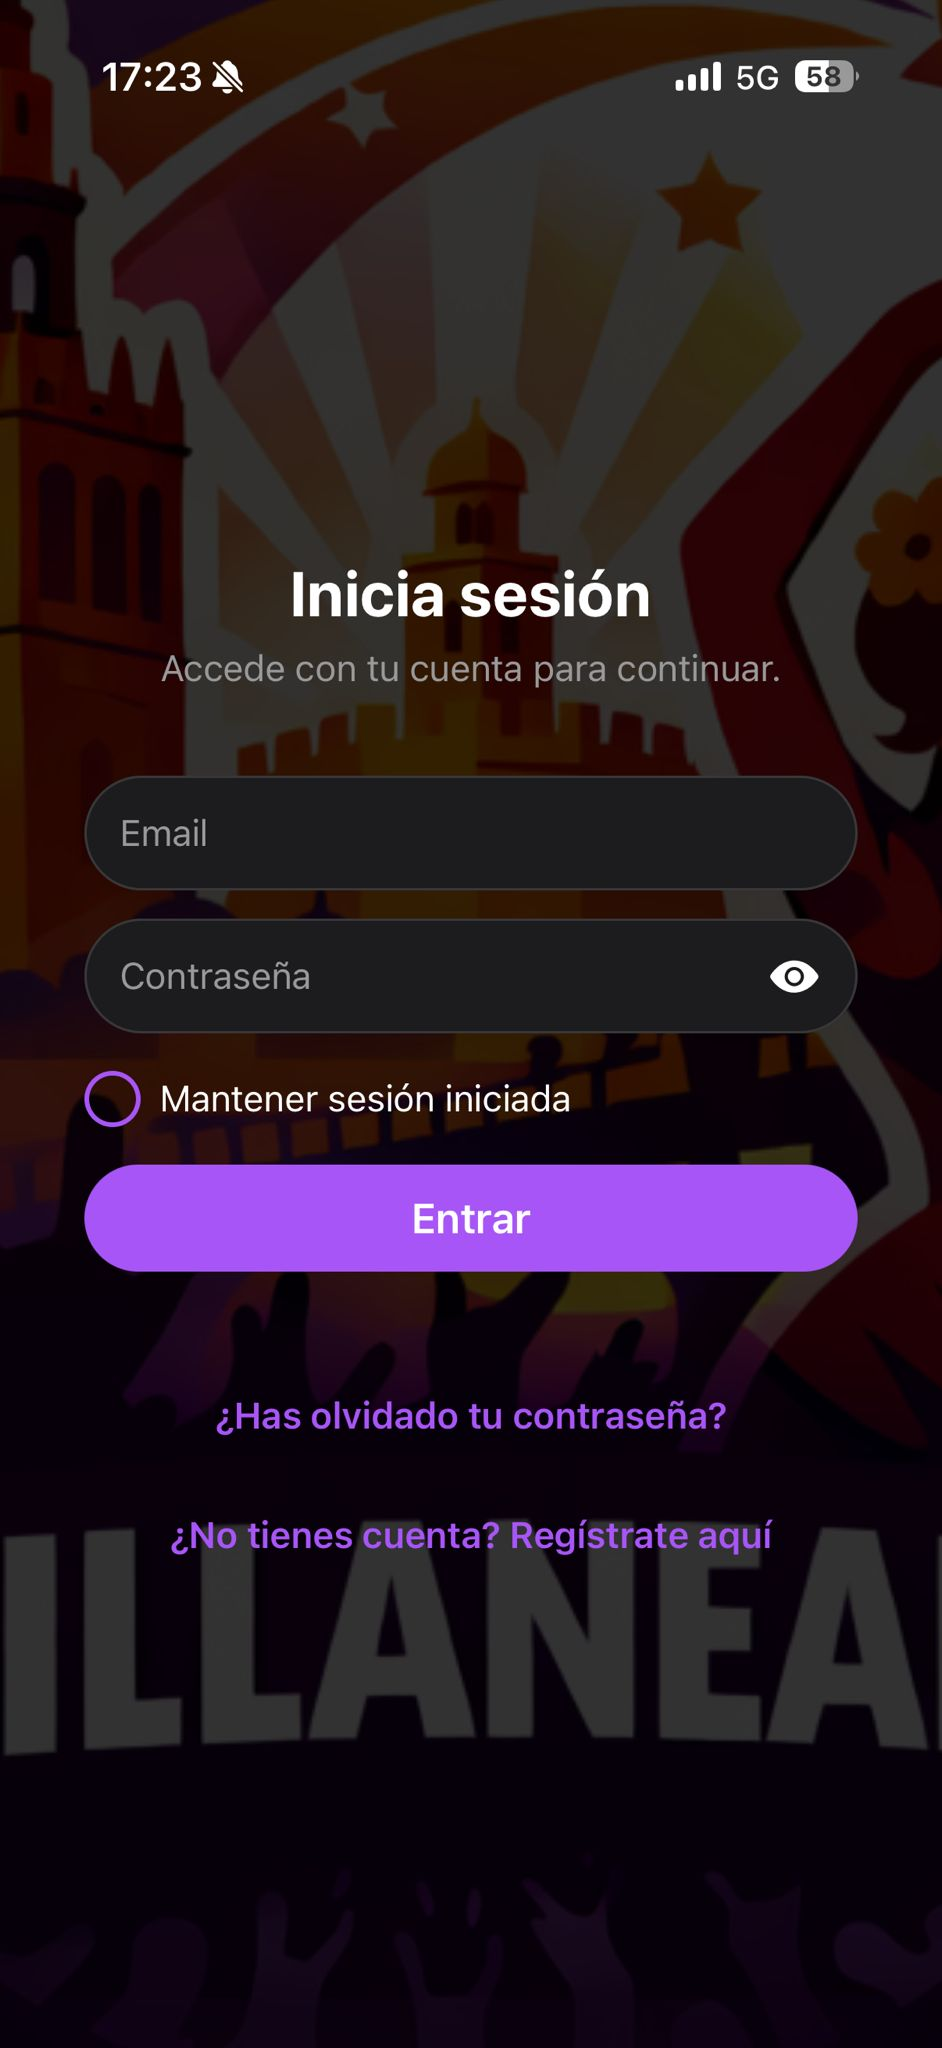
\includegraphics[width=\linewidth]{figures/paso1/iniciar_sesion.png}
        \caption{Iniciar sesión}
    \end{subfigure}
    \caption{Acceso a la aplicación}
\end{figure}

\clearpage

\subsection{Gestión del perfil (para todos los roles)}

Tras iniciar sesión, el usuario puede abrir el menú lateral pulsando el icono de tres líneas situado en la esquina superior izquierda de la página principal. Este panel agrupa en su parte superior la información del usuario, los botones de selección del tema visual (\textit{Claro} y \textit{Oscuro}) y, justo debajo del avatar, un icono de lápiz que abre la pantalla de edición del perfil. El mismo menú incluye, en su parte inferior, el botón de cierre de sesión.

La pantalla de edición del perfil se compone de varios bloques que el usuario puede recorrer mediante desplazamiento vertical. En la parte superior aparece la fotografía de perfil: al pulsar sobre ella se abre la galería del dispositivo para seleccionar una nueva imagen, que se recorta en formato cuadrado y se sube automáticamente al guardarla; si ya existía una foto previa, junto a ella aparece un botón rojo \textit{Quitar foto} para eliminarla. A continuación se editan el nombre y el correo electrónico mediante dos campos de texto. Más abajo, un recuadro informativo explica el uso de la ubicación: el usuario puede escribir una dirección o lugar en el campo de búsqueda y pulsar la lupa para localizarlo, o bien tocar directamente sobre el mapa para fijar el punto deseado, que queda marcado con un pin. Las coordenadas seleccionadas se muestran debajo del mapa y, si se desea descartar la ubicación, basta con pulsar el icono rojo de aspa situado junto a ellas.

En el bloque de intereses se listan las categorías disponibles como etiquetas pulsables; al tocar una etiqueta esta se activa o desactiva, quedando resaltadas las seleccionadas. Estos intereses condicionan posteriormente las recomendaciones de eventos. Bajo este bloque, el botón principal \textit{Guardar} confirma todos los cambios y vuelve a la pantalla anterior. El botón secundario \textit{Cambiar contraseña} abre una pantalla independiente desde la que puede modificarse la contraseña actual. A continuación se muestra el selector de idioma, con dos opciones (\textit{Español} e \textit{English}) que cambian el idioma de la interfaz al pulsarlas. Por último, en la parte inferior aparece el botón rojo \textit{Eliminar cuenta}: al pulsarlo se solicita confirmación mediante un cuadro de diálogo y, si se acepta, la cuenta se elimina de forma definitiva tanto en la aplicación como en el servicio de autenticación. Si el inicio de sesión es demasiado antiguo, la aplicación pide volver a autenticarse antes de completar el borrado.

\bigskip

\textbf{Validaciones y recomendaciones:}
\begin{itemize}[leftmargin=1.5em]
\item Se recomienda indicar una ubicación para habilitar todas las funciones de proximidad.
\item Los datos modificados deben guardarse correctamente antes de salir.
\item El correo electrónico debe mantener un formato válido.
\end{itemize}

\begin{figure}[H]
    \centering
    \begin{subfigure}{0.285\linewidth}
        \centering
        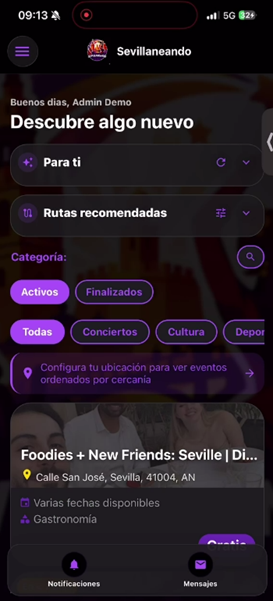
\includegraphics[width=\linewidth]{figures/home_screen.png}
        \caption{Página principal}
    \end{subfigure}
    \hspace{0.02\linewidth}
    \begin{subfigure}{0.3\linewidth}
        \centering
        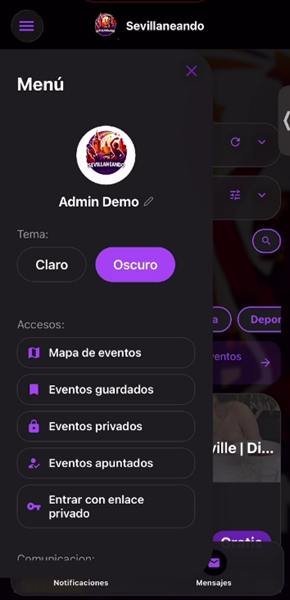
\includegraphics[width=\linewidth]{figures/lateral_menu.png}
        \caption{Menú lateral}
    \end{subfigure}
    \hspace{0.02\linewidth}
    \begin{subfigure}{0.29\linewidth}
        \centering
        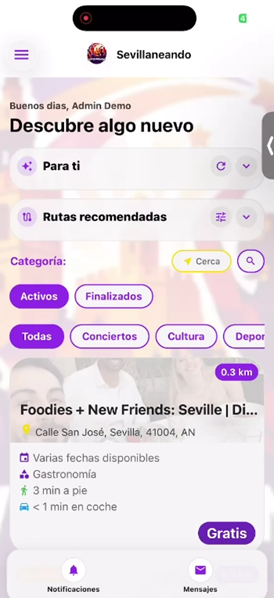
\includegraphics[width=\linewidth]{figures/paso2/modo_claro.png}
        \caption{Modo claro}
    \end{subfigure}
    \caption{Acceso y opciones del perfil}
\end{figure}

\begin{figure}[H]
    \centering
    \begin{subfigure}{0.33\linewidth}
        \centering
        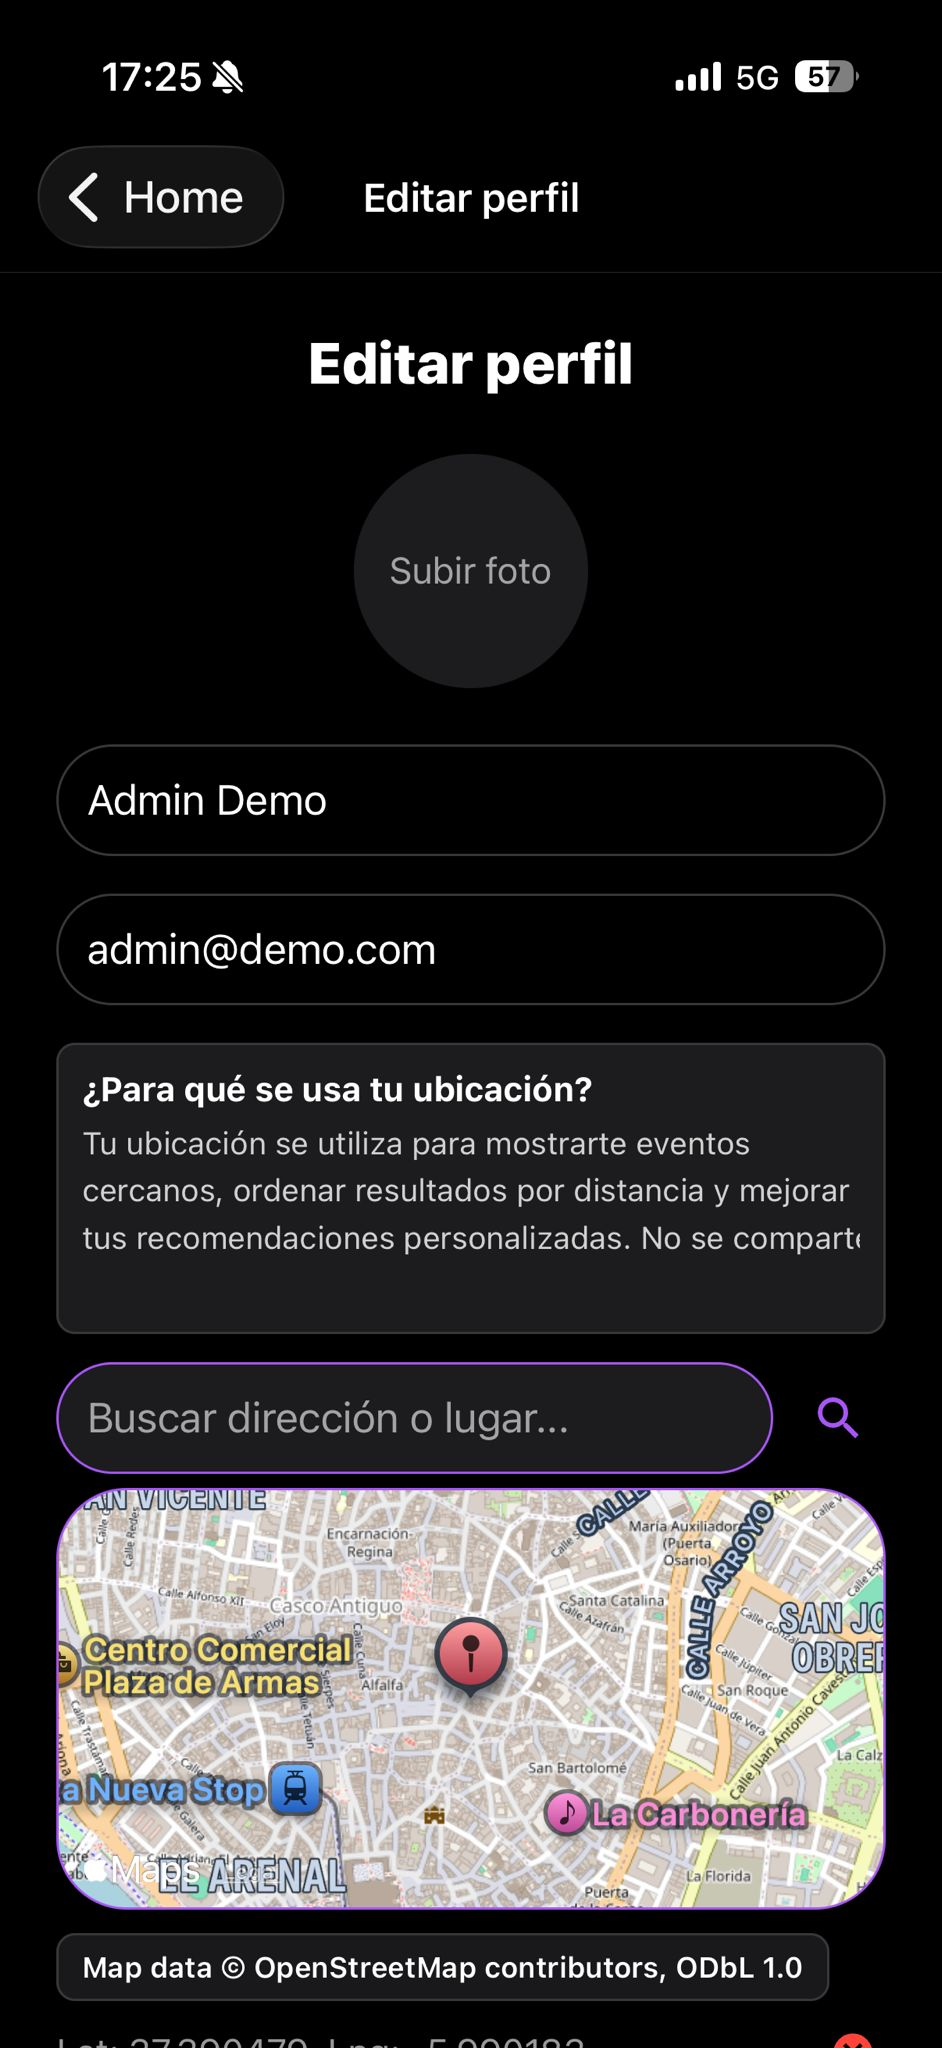
\includegraphics[width=\linewidth]{figures/paso2/edit_profile.png}
        \caption{Editar perfil 1}
    \end{subfigure}
    \hspace{0.02\linewidth}
    \begin{subfigure}{0.33\linewidth}
        \centering
        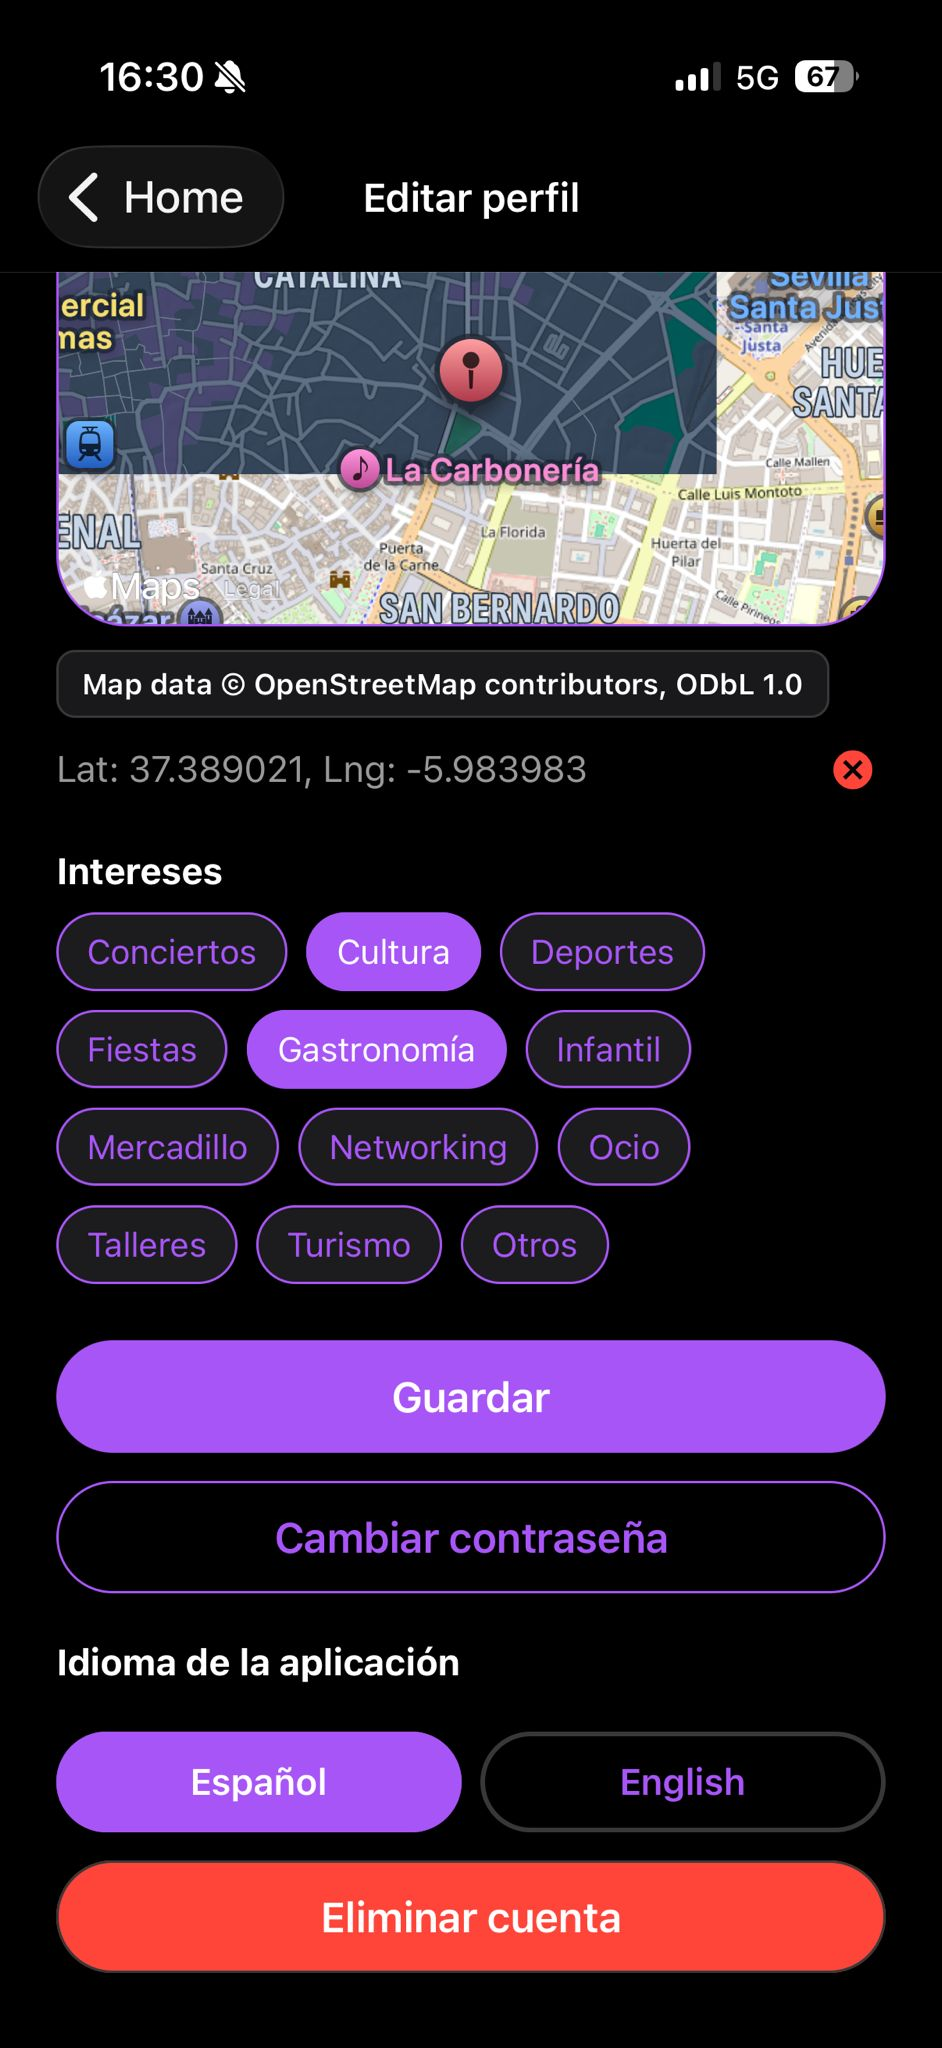
\includegraphics[width=\linewidth]{figures/paso2/edit_profile2.png}
        \caption{Editar perfil 2}
    \end{subfigure}
    \hspace{0.02\linewidth}
    \begin{subfigure}{0.34\linewidth}
        \centering
        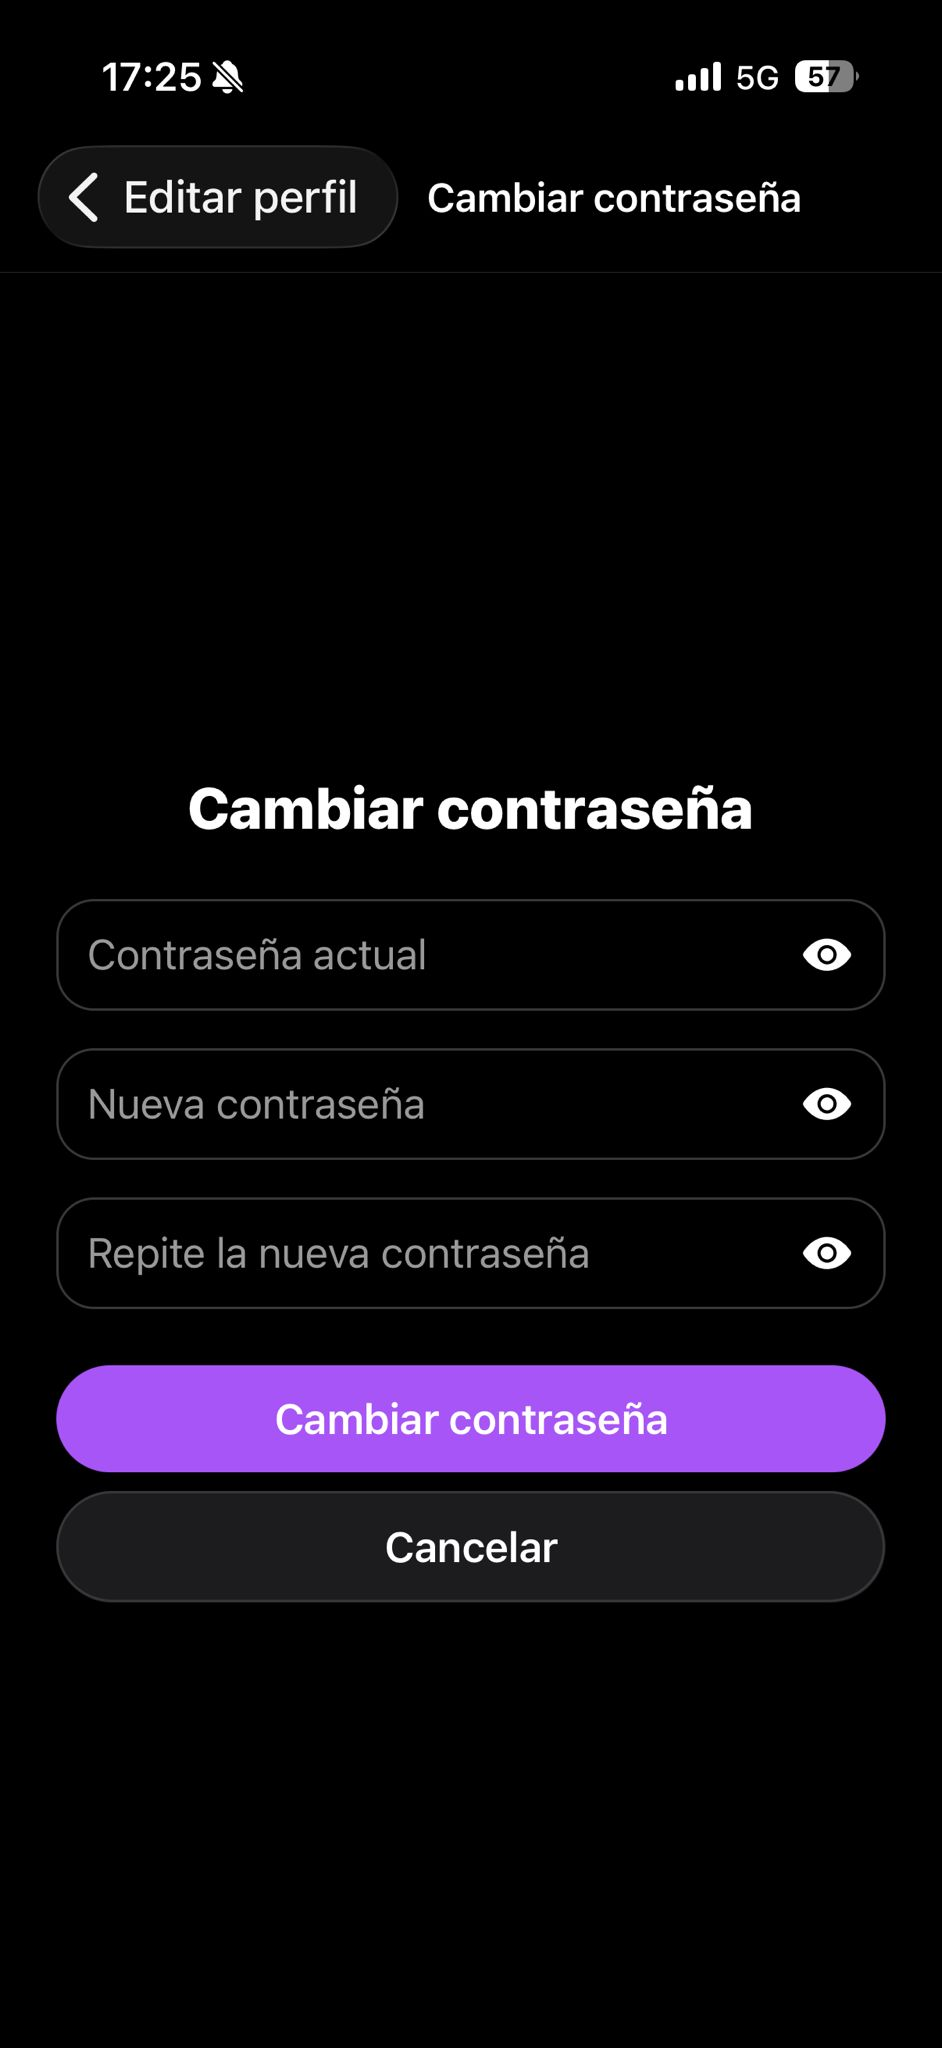
\includegraphics[width=\linewidth]{figures/paso2/edit_profile3.png}
        \caption{Cambiar contraseña}
    \end{subfigure}
    \caption{Gestión del perfil}
\end{figure}

\clearpage

\subsection{Mapa de eventos (para todos los roles)}

La aplicación permite consultar los eventos en un mapa interactivo, lo que resulta útil para usuarios que desean localizar actividades próximas a su ubicación. Para acceder a esta funcionalidad, el usuario debe abrir el menú lateral desde la esquina superior izquierda y pulsar la opción \textit{Mapa de eventos}. La pantalla se carga centrada en la ubicación que el usuario tiene configurada en su perfil; si todavía no ha indicado ninguna, el mapa se centra en Sevilla y un aviso en la parte inferior recuerda que es necesario configurar la ubicación para que las funciones de proximidad tengan efecto.

Si el usuario tiene ubicación configurada, su posición se representa con un marcador morado distintivo y a su alrededor se dibuja un círculo translúcido que delimita el radio de búsqueda actual. Los eventos aparecen como chinchetas coloreadas en función de su distancia: verde cuando se encuentran a menos de un kilómetro, amarillo entre uno y tres, naranja entre tres y cinco, y rojo por encima de cinco; los eventos cuya distancia no puede calcularse aparecen en morado. En la parte inferior de la pantalla se muestra un recuadro con el radio actual en kilómetros y una barra deslizante que permite modificarlo entre doscientos metros y cinco kilómetros; el círculo del mapa se actualiza en tiempo real conforme se ajusta este valor.

Al pulsar sobre la chincheta de un evento aparece una tarjeta resumen con el título, una breve descripción, la dirección y la distancia. En esta tarjeta, el botón \textit{Ver detalles} (o un toque adicional sobre la propia tarjeta en iOS) abre la pantalla de detalle completo del evento. Para cerrar la tarjeta sin abandonar el mapa, basta con pulsar el icono de aspa que aparece en su esquina. Para salir de la pantalla del mapa se utiliza el botón circular con icono de cierre situado en la esquina superior derecha, que devuelve al usuario a la página principal.

\bigskip

\textbf{Aspectos a tener en cuenta:}
\begin{itemize}[leftmargin=1.5em]
\item Es necesario haber configurado una ubicación previamente en el perfil.
\end{itemize}

\begin{figure}[H]
    \centering
    \begin{subfigure}{0.3\linewidth}
        \centering
        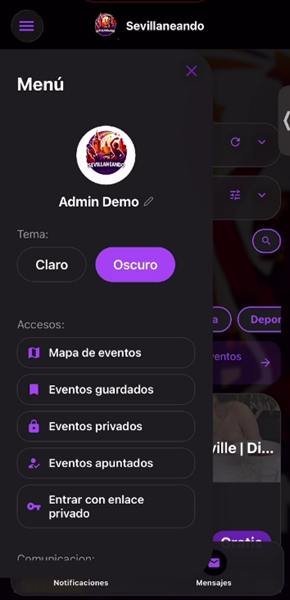
\includegraphics[width=\linewidth]{figures/lateral_menu.png}
        \caption{Menú lateral}
    \end{subfigure}
    \hspace{0.01\linewidth}
    \begin{subfigure}{0.293\linewidth}
        \centering
        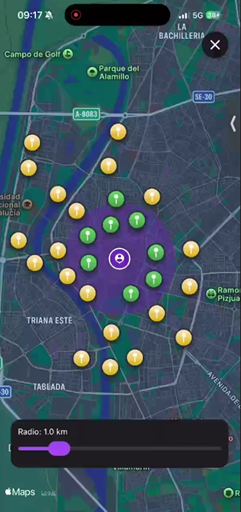
\includegraphics[width=\linewidth]{figures/paso3/mapa1.png}
        \caption{Eventos en el mapa}
    \end{subfigure}
    \hspace{0.01\linewidth}
    \begin{subfigure}{0.29\linewidth}
        \centering
        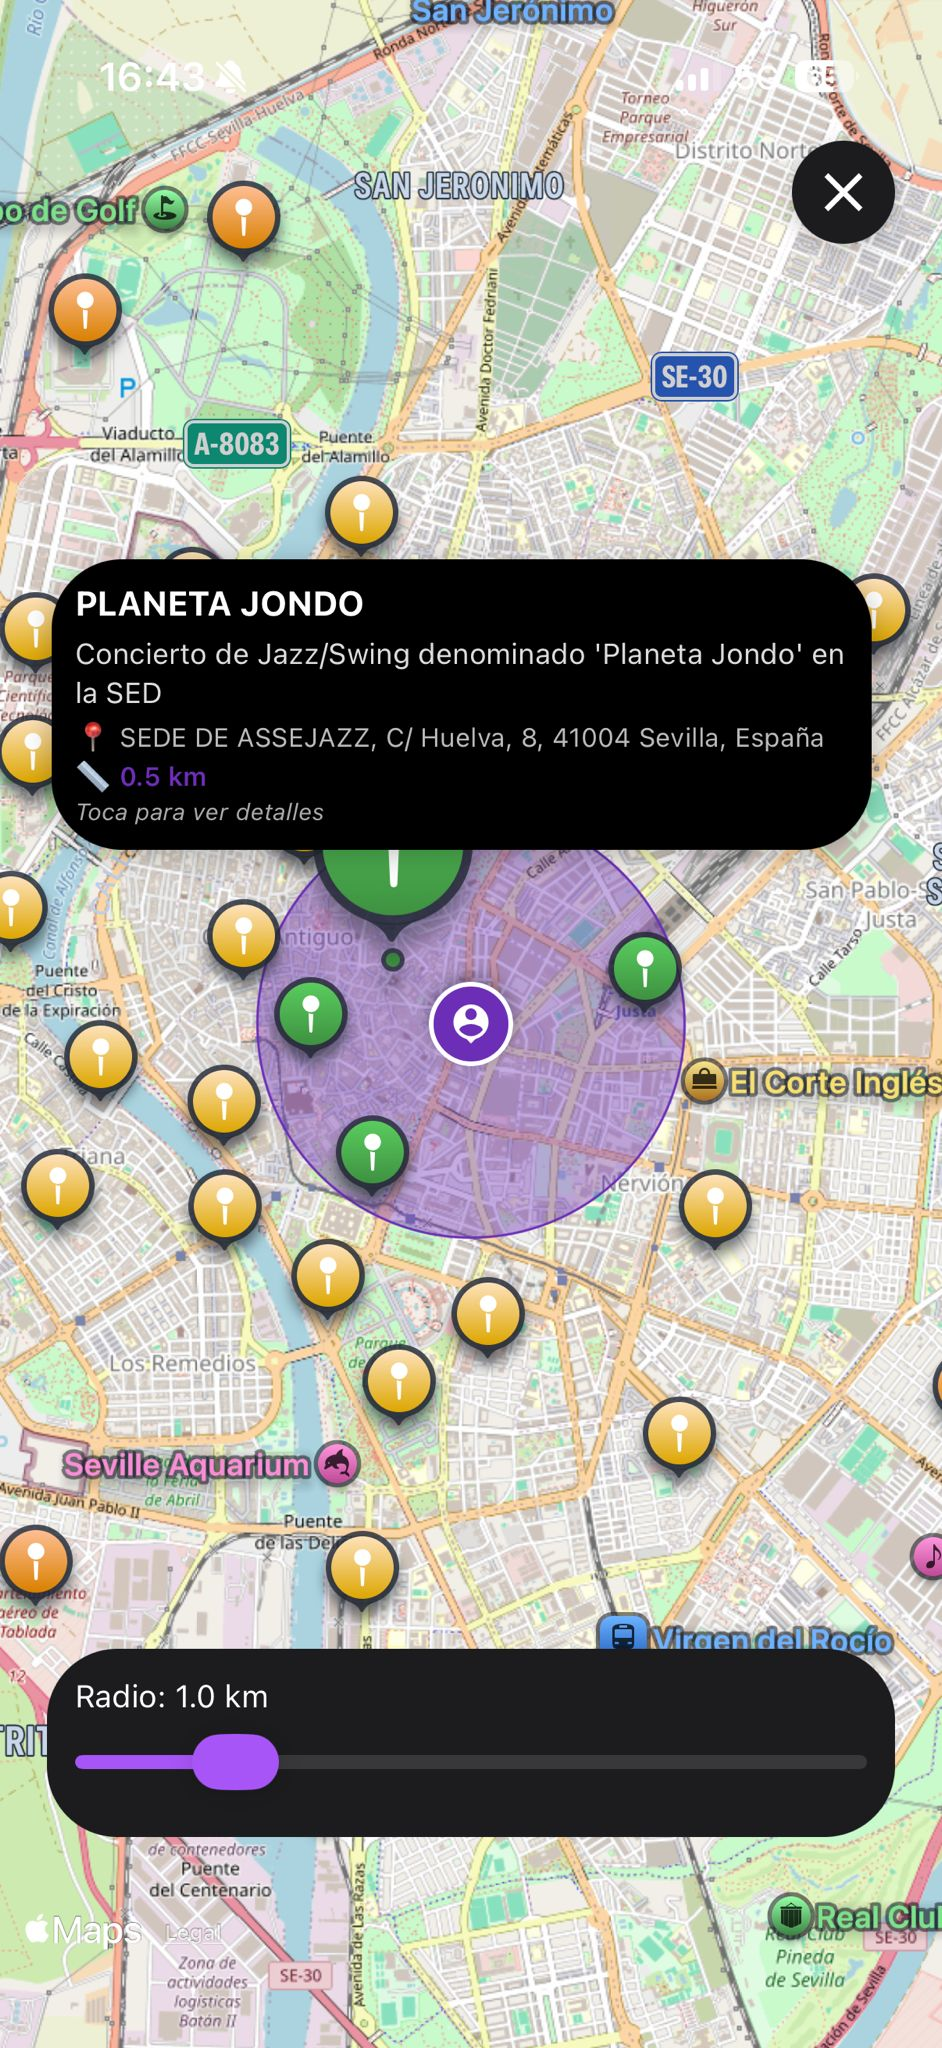
\includegraphics[width=\linewidth]{figures/paso3/mapa2.png}
        \caption{Etiqueta del evento}
    \end{subfigure}
    \caption{Mapa de eventos}
\end{figure}

\clearpage

\subsection{Página principal y filtros (para todos los roles)}

La página principal es el espacio central de consulta de la aplicación y se muestra automáticamente tras iniciar sesión. En su parte superior aparece un saludo personalizado con el nombre del usuario que cambia según la hora del día, y debajo se sitúa una barra horizontal con las categorías disponibles, que el usuario puede arrastrar lateralmente para recorrerlas y pulsar para activar una categoría como filtro. Manteniendo pulsada una categoría es posible reordenarlas: al soltar, el nuevo orden queda guardado en el perfil para que las preferidas aparezcan primero en futuros accesos. La etiqueta \textit{Todas} restablece la vista sin filtro de categoría.

Bajo las categorías se encuentran dos botones de filtrado rápido. El primero, \textit{Cerca}, se ilumina cuando se activa y muestra únicamente los eventos dentro del radio configurado; al hacerlo aparece sobre el listado una fila de valores de radio en kilómetros que el usuario puede pulsar para ajustar la distancia. Este filtro requiere tener ubicación configurada en el perfil; si no la hay, la aplicación muestra un mensaje que enlaza directamente con la pantalla de edición del perfil. El segundo botón abre el buscador avanzado en una ventana emergente que permite escribir un texto libre para buscar por título o descripción, definir un precio mínimo y máximo, y delimitar un intervalo de fechas mediante dos selectores de calendario. Dentro del buscador, el botón \textit{Buscar} aplica los criterios y \textit{Limpiar filtros} los descarta.

Entre los filtros y el listado aparecen dos pestañas, \textit{Eventos activos} y \textit{Eventos finalizados}, que separan los eventos vigentes de los ya finalizados. Cada evento se muestra como una tarjeta con su imagen de portada, título, dirección, fecha y categoría; al pulsar la tarjeta se accede a la pantalla de detalle. Por encima del listado, cuando hay datos suficientes, la página integra dos secciones de recomendaciones (eventos y rutas) que se describen más adelante. En la parte inferior de la pantalla se sitúa una barra fija con accesos directos a notificaciones, mensajes, creación de evento, moderación (si el rol lo permite) y amigos.

\bigskip

\textbf{Aspectos a tener en cuenta:}
\begin{itemize}[leftmargin=1.5em]
\item Los eventos finalizados siguen siendo visibles, pero no admiten inscripción.
\item El filtrado por cercanía requiere ubicación.
\item Las categorías pueden organizarse arrastándolas horizontalmente para dejar primero las favoritas.
\end{itemize}

\begin{figure}[H]
    \centering
    \begin{subfigure}{0.3\linewidth}
        \centering
        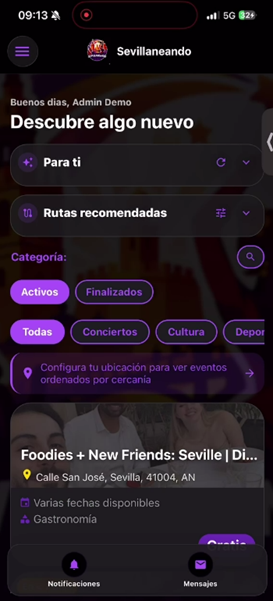
\includegraphics[width=\linewidth]{figures/home_screen.png}
        \caption{Página principal}
    \end{subfigure}
    \hspace{0.01\linewidth}
    \begin{subfigure}{0.324\linewidth}
        \centering
        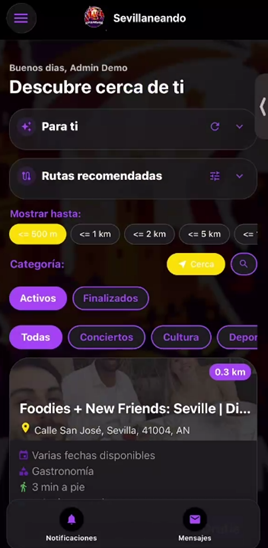
\includegraphics[width=\linewidth]{figures/paso4/cerca.png}
        \caption{Búsqueda por cercanía}
    \end{subfigure}
    \hspace{0.01\linewidth}
    \begin{subfigure}{0.321\linewidth}
        \centering
        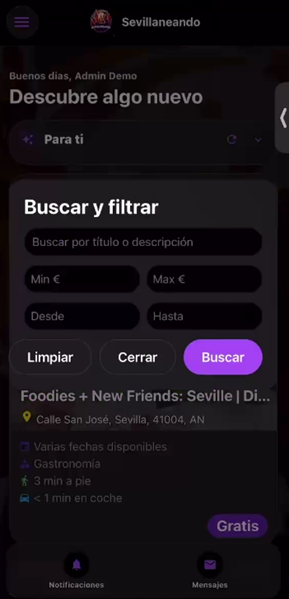
\includegraphics[width=\linewidth]{figures/paso4/busqueda.png}
        \caption{Buscador avanzado}
    \end{subfigure}
    \caption{Filtros de búsqueda}
\end{figure}

\clearpage

\subsection{Detalle de evento}

La pantalla de detalle se abre al pulsar cualquier evento desde la página principal, el mapa, un listado personalizado o una notificación. En la parte superior aparece un carrusel de imágenes que puede desplazarse horizontalmente con el dedo, y bajo este se muestran el título, la dirección, la descripción, el rango de fechas, la duración total, el tiempo restante hasta el inicio o el final, la categoría y, si procede, la recurrencia y la valoración media en estrellas. El precio se muestra destacado en un recuadro morado en la parte inferior derecha del bloque informativo. Si la descripción contiene un enlace a la fuente original (común en eventos importados por scraping), este aparece resaltado y abre el navegador del dispositivo al pulsarlo.

Más abajo se incluye un pequeño mapa centrado en la ubicación del evento; por defecto está bloqueado para no interferir con el desplazamiento de la pantalla, pero pulsando el icono de candado de su esquina puede desbloquearse para hacer zoom o moverlo. Al pulsar la chincheta del mapa se muestra una etiqueta con el título y un enlace que abre la ubicación en Google Maps o Apple Maps según el sistema operativo del dispositivo.

A continuación se muestra el panel \textit{Acciones}, organizado en botones. El botón principal permite apuntarse al evento o, si el usuario ya está apuntado, eliminar su inscripción; este botón queda deshabilitado en eventos finalizados. Bajo él hay dos filas de botones secundarios: \textit{Asistentes}, que abre una ventana emergente con la lista de personas apuntadas (cada nombre es pulsable y abre el perfil correspondiente); \textit{Abrir mapa}, que lanza la aplicación de mapas externa con la dirección del evento ya cargada; \textit{Guardar} (o \textit{Quitar de guardados}), que añade el evento al listado de eventos guardados y alimenta el sistema de recomendaciones; y \textit{Compartir} (o \textit{Invitar} en eventos privados), que abre el menú de compartir nativo del dispositivo con un mensaje que incluye el título, fecha, dirección, categoría, precio y enlace al evento. En el caso de eventos privados, este botón solo está disponible para el creador, y al pulsarlo se genera el enlace de acceso compartible. Por último, el botón \textit{Valorar} (o \textit{Editar valoración} si ya existe una) abre una ventana emergente con cinco estrellas pulsables para indicar la puntuación y un campo de texto opcional para escribir un comentario; al pulsar \textit{Enviar} la valoración se guarda y la lista de opiniones del propio evento se actualiza automáticamente.

Bajo el panel de acciones se muestra la sección \textit{Opiniones}, donde aparecen las valoraciones de otros usuarios con su foto, nombre, fecha, número de estrellas y comentario. Al pulsar sobre el nombre o la foto se accede al perfil público del autor de la opinión.

En la esquina superior derecha de la pantalla aparece un icono de bocadillo que abre el chat del evento, accesible a todos los participantes. El chat se despliega como un panel deslizable sobre el detalle, con el historial de mensajes en orden cronológico. Cada mensaje muestra el avatar del autor, su nombre y la hora; al pulsar sobre el avatar o el nombre se abre su perfil, y al pulsar el icono de sobre situado junto al mensaje se inicia un chat privado. Para enviar un mensaje se escribe en el campo inferior y se pulsa \textit{Enviar}; junto al campo hay dos botones para adjuntar una imagen desde la galería o tomar una foto directamente con la cámara. Al pulsar sobre una imagen recibida se abre a pantalla completa con posibilidad de hacer zoom con dos dedos. Manteniendo pulsado un mensaje propio aparece la opción de eliminarlo. Si el usuario tiene rol de moderador o administrador, en lugar del icono de bocadillo se muestra también un icono de lápiz junto a él, que abre la pantalla de edición moderada del evento.

\bigskip

\textbf{Aspectos a tener en cuenta:}
\begin{itemize}[leftmargin=1.5em]
\item Algunas acciones solo están disponibles en eventos activos (inscribirse) y públicos (compartir).
\item La interacción con el evento influye en futuras recomendaciones.
\item Desde asistentes, perfiles del chat y perfiles de usuario puede iniciarse mensajería privada.
\end{itemize}

\begin{figure}[H]
    \centering
    \begin{subfigure}{0.3\linewidth}
        \centering
        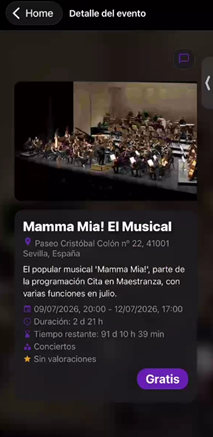
\includegraphics[width=\linewidth]{figures/paso5/event_detail.png}
        \caption{Detalles del evento}
    \end{subfigure}
    \hspace{0.02\linewidth}
    \begin{subfigure}{0.305\linewidth}
        \centering
        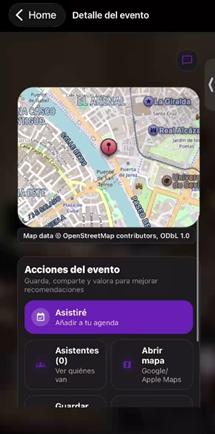
\includegraphics[width=\linewidth]{figures/paso5/event_detail2.png}
        \caption{Detalles del evento 2}
    \end{subfigure}
    \hspace{0.02\linewidth}
    \begin{subfigure}{0.306\linewidth}
        \centering
        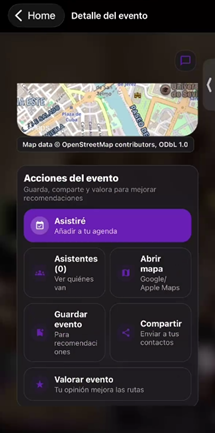
\includegraphics[width=\linewidth]{figures/paso5/event_detail3.png}
        \caption{Acciones del evento}
    \end{subfigure}
    \caption{Pantalla del evento}
\end{figure}

\begin{figure}[H]
    \centering
    \begin{subfigure}{0.35\linewidth}
        \centering
        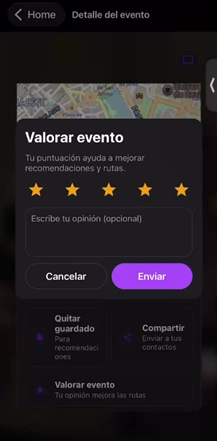
\includegraphics[width=\linewidth]{figures/paso5/valoracion.png}
        \caption{Valorar evento}
    \end{subfigure}
    \hspace{0.02\linewidth}
    \begin{subfigure}{0.352\linewidth}
        \centering
        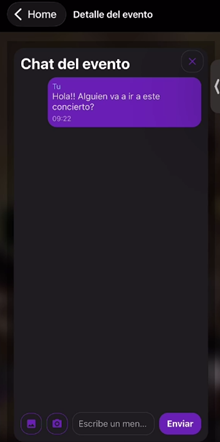
\includegraphics[width=\linewidth]{figures/paso5/chat_evento.png}
        \caption{Chat del evento}
    \end{subfigure}
    \caption{Interacción dentro del evento}
\end{figure}

\clearpage

\subsection{Listados de eventos}

La aplicación organiza determinados eventos en listados personalizados accesibles desde el menú lateral. Cada listado responde a un tipo concreto de interacción previa del usuario y se actualiza automáticamente cada vez que se entra en él.

Para consultar los eventos guardados, el usuario debe abrir el menú lateral y pulsar \textit{Eventos guardados}. La pantalla muestra el listado completo de los eventos que el usuario ha marcado pulsando el botón \textit{Guardar} desde el panel de acciones del detalle del evento. Cada elemento se presenta como una tarjeta con la imagen, el título, la fecha, la dirección y la categoría, y al pulsar sobre ella se abre el detalle correspondiente. Para retirar un evento del listado basta con volver a su detalle y pulsar nuevamente el botón, que ahora aparece como \textit{Quitar de guardados}.

Los eventos a los que el usuario se ha apuntado se consultan desde la opción \textit{Eventos apuntados} del menú lateral. En esta pantalla se muestran únicamente las inscripciones activas, ordenadas por fecha. La inscripción y la cancelación se realizan siempre desde el botón principal del panel de acciones del detalle del evento.

El calendario es accesible desde la opción \textit{Calendario} del menú lateral y muestra una vista mensual en la que los días con eventos a los que el usuario está apuntado aparecen marcados con un punto morado. Pulsando sobre un día concreto se selecciona y, bajo el calendario, se despliega la lista de eventos cuyo inicio coincide con esa fecha. Cada elemento de la lista incluye la hora de comienzo y el título, y al pulsarlo se abre el detalle del evento. Los controles de cabecera del calendario permiten avanzar y retroceder entre meses.

\begin{figure}[H]
    \centering
    \begin{subfigure}[b]{0.35\linewidth}
        \centering
        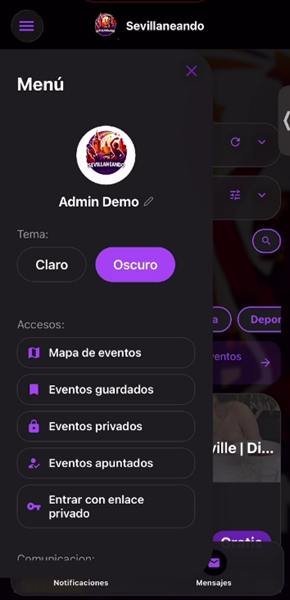
\includegraphics[height=9.5cm,keepaspectratio]{figures/lateral_menu.png}
        \caption{Menú lateral}
    \end{subfigure}
    \hspace{0.1\linewidth}
    \begin{subfigure}[b]{0.35\linewidth}
        \centering
        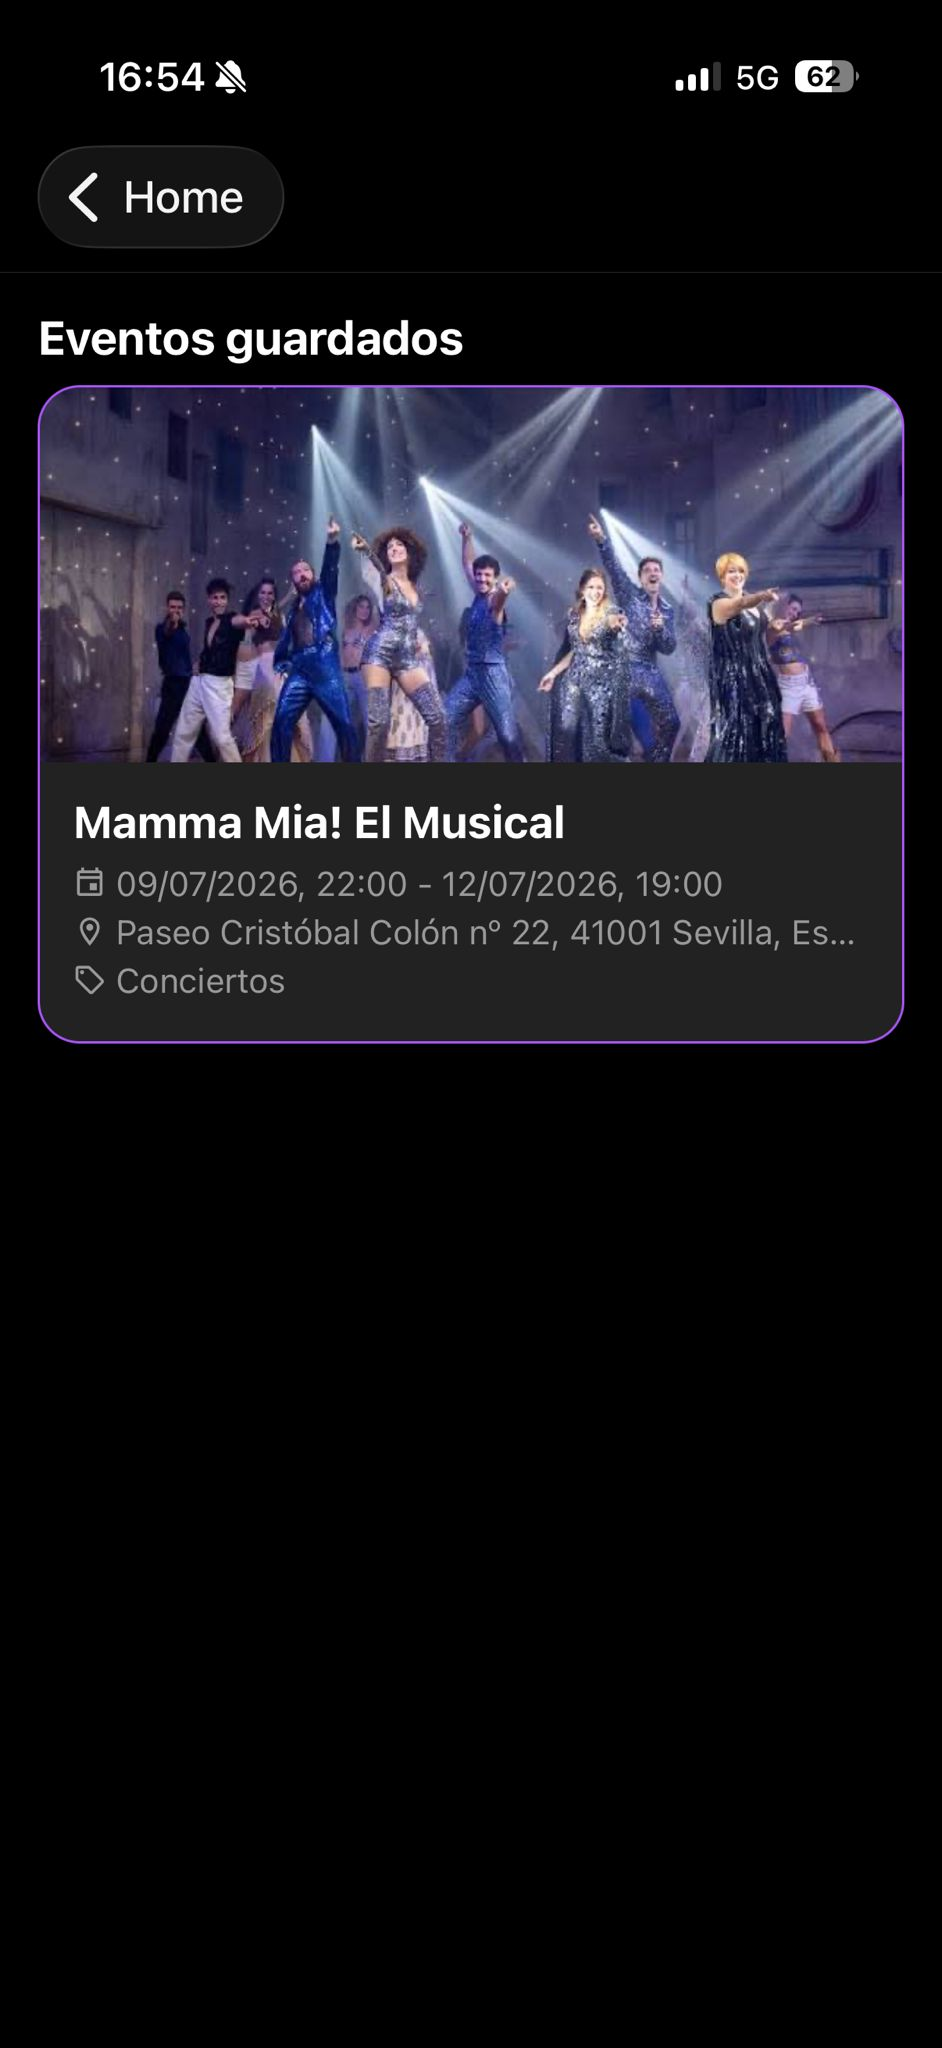
\includegraphics[height=9.5cm,keepaspectratio]{figures/paso6/eventos_guardados.png}
        \caption{Eventos guardados}
    \end{subfigure}
    \caption{Listado de eventos guardados}
\end{figure}

\begin{figure}[H]
    \centering
    \begin{subfigure}[b]{0.3\linewidth}
        \centering
        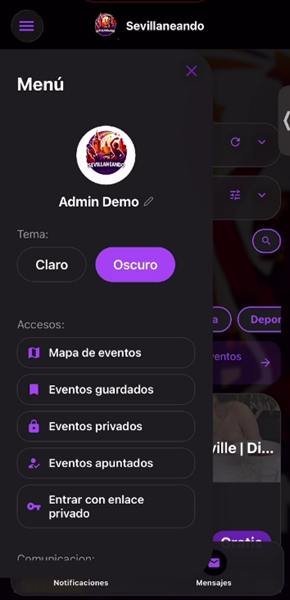
\includegraphics[height=9.5cm,keepaspectratio]{figures/lateral_menu.png}
        \caption{Menú lateral}
    \end{subfigure}
    \hspace{0.1\linewidth}
    \begin{subfigure}[b]{0.3\linewidth}
        \centering
        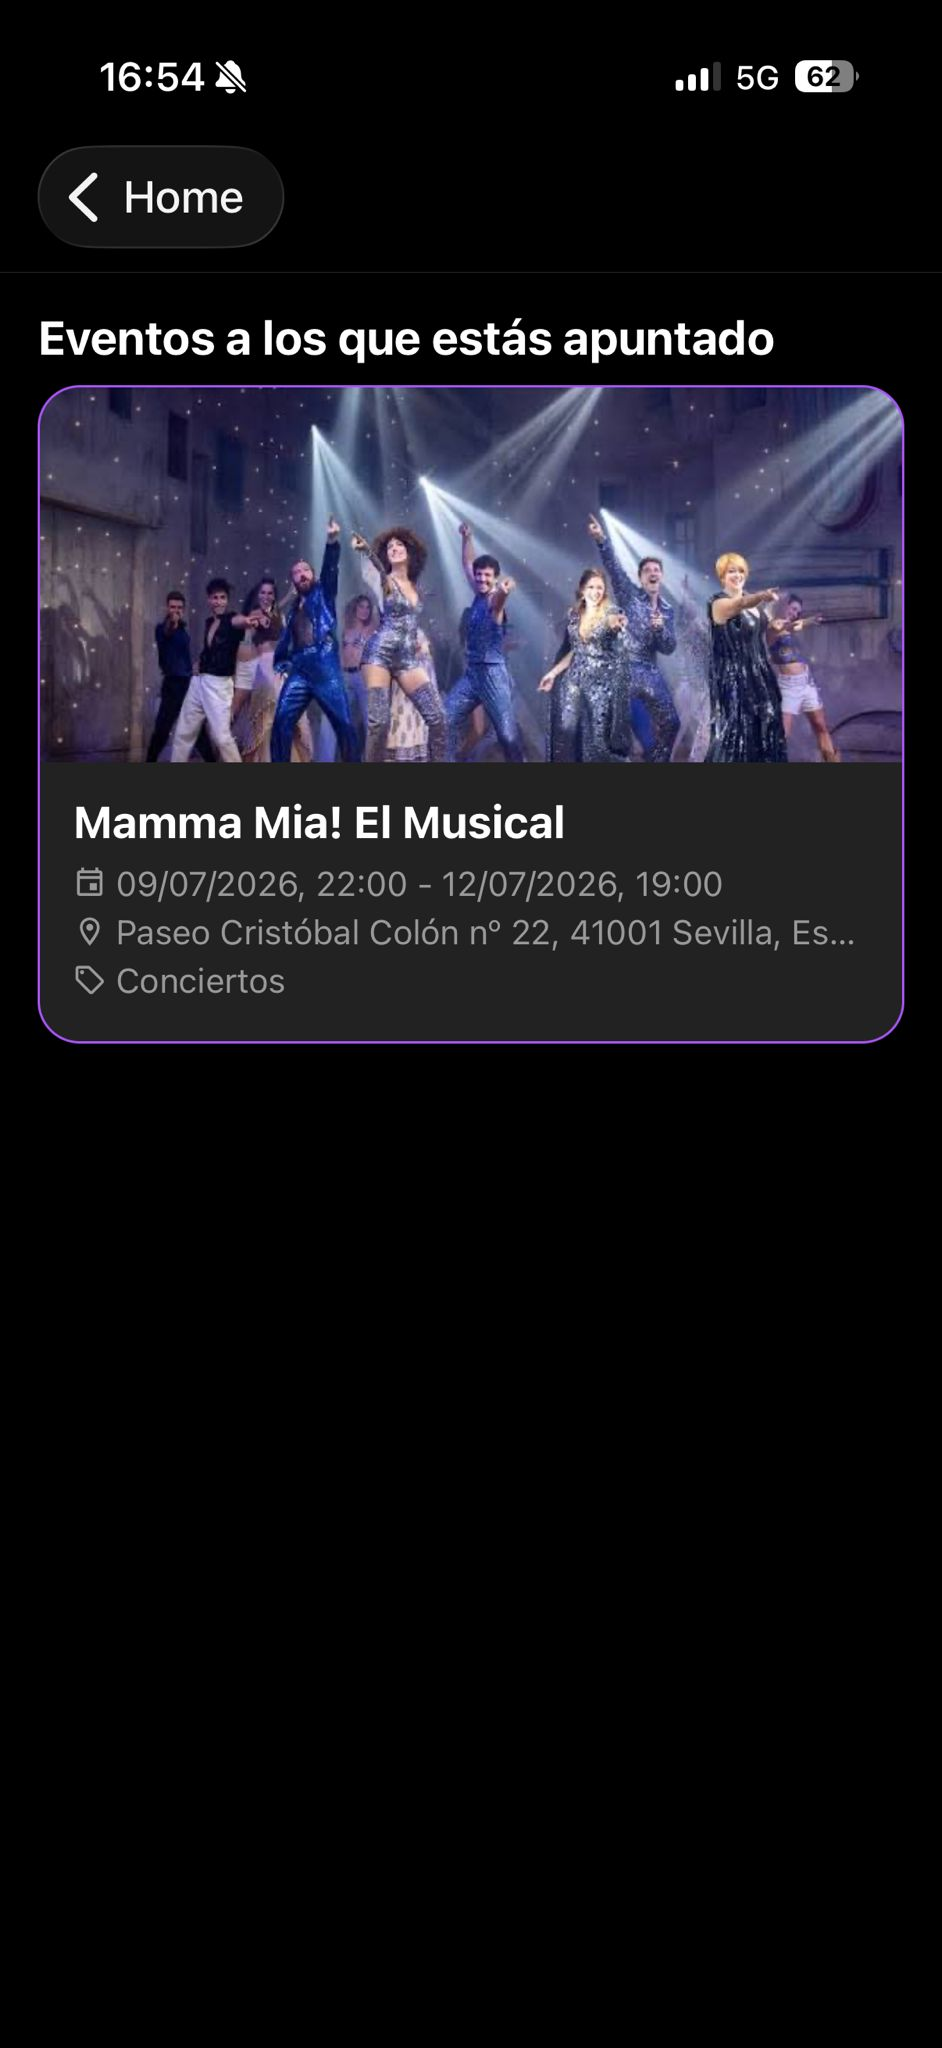
\includegraphics[height=9.5cm,keepaspectratio]{figures/paso6/eventos_apuntados.png}
        \caption{Eventos apuntados}
    \end{subfigure}
    \caption{Listado de eventos apuntados}
\end{figure}

\begin{figure}[H]
    \centering
    \begin{subfigure}{0.3\linewidth}
        \centering
        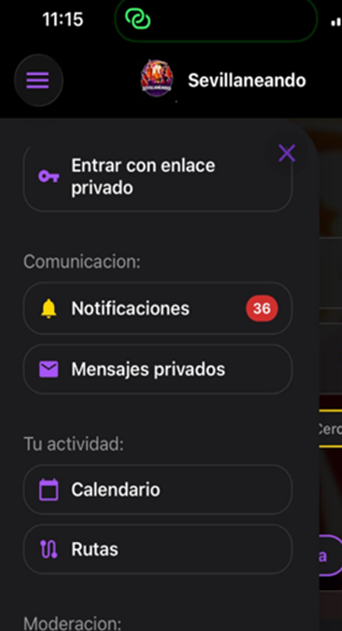
\includegraphics[width=\linewidth]{figures/paso6/lateral_menu2.png}
        \caption{Menú lateral}
    \end{subfigure}
    \hspace{0.1\linewidth}
    \begin{subfigure}{0.26\linewidth}
        \centering
        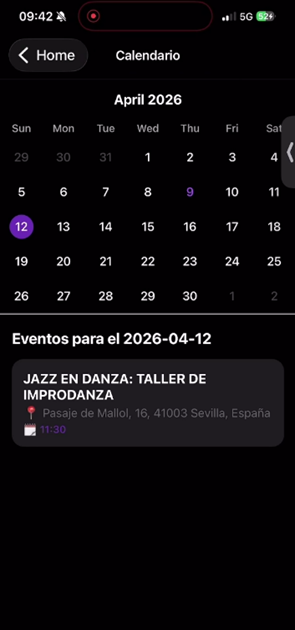
\includegraphics[width=\linewidth]{figures/paso6/calendario.png}
        \caption{Calendario}
    \end{subfigure}
    \caption{Calendario de eventos}
\end{figure}

\clearpage

\subsection{Gestión de administrador (rol de administrador)}

El rol de administrador dispone de funcionalidades específicas para mantener la organización global del sistema. Tras iniciar sesión con una cuenta de administrador, en el menú lateral aparece la opción \textit{Administración}, que abre el panel principal de gestión, así como una entrada adicional para la gestión de categorías.

El panel de administración se organiza en tres pestañas que pueden alternarse pulsando la barra superior. La pestaña \textit{Estadísticas} es la que se muestra por defecto y presenta una serie de tarjetas con los principales indicadores del sistema: el número total de usuarios registrados, el total de eventos, los eventos aprobados, pendientes de moderación y rechazados, y, en un bloque diferenciado, el reparto entre eventos importados automáticamente por scraping y eventos creados manualmente por los propios usuarios. Esta información se actualiza al volver a entrar en el panel.

La pestaña \textit{Usuarios} muestra la lista completa de cuentas con su foto, nombre, correo y rol actual. Al pulsar sobre un usuario se abre una ventana emergente desde la que el administrador puede asignar uno de los tres roles disponibles, \textit{Usuario}, \textit{Moderador} o \textit{Administrador}, pulsando el botón correspondiente, o eliminar la cuenta por completo mediante el botón rojo de borrado. Ambas acciones piden confirmación antes de aplicarse, y al completarse, el listado se actualiza automáticamente con el nuevo estado.

La pestaña \textit{Scraping} contiene el botón \textit{Restablecer eventos importados}. Al pulsarlo se solicita confirmación porque la operación borra todos los eventos previamente importados y vuelve a ejecutar los scrapers de las fuentes configuradas. La operación puede tardar varios minutos y al finalizar se muestra un resumen con el número de eventos eliminados y el número de eventos recuperados. Es recomendable utilizar esta funcionalidad solo cuando se detectan inconsistencias claras en el catálogo externo, ya que durante su ejecución la página principal puede mostrar resultados parciales.

La gestión de categorías se realiza desde una pantalla independiente accesible también desde el menú lateral. En ella se listan todas las categorías existentes con su nombre y descripción. Mediante el botón flotante con el símbolo \textit{+} se abre un formulario para crear una nueva categoría rellenando estos dos campos, y pulsando sobre una categoría existente se abre el mismo formulario en modo edición. Cada categoría incluye también un botón de eliminación; los eventos asociados a una categoría borrada se reasignan automáticamente a la categoría \textit{Otros} para no perderlos.

\bigskip

\textbf{Credenciales de prueba:}
\begin{itemize}[leftmargin=1.5em]
\item Email: \texttt{admin@demo.com}
\item Contraseña: \texttt{administrador}
\end{itemize}

\begin{figure}[H]
    \centering
    \begin{subfigure}{0.30\linewidth}
        \centering
        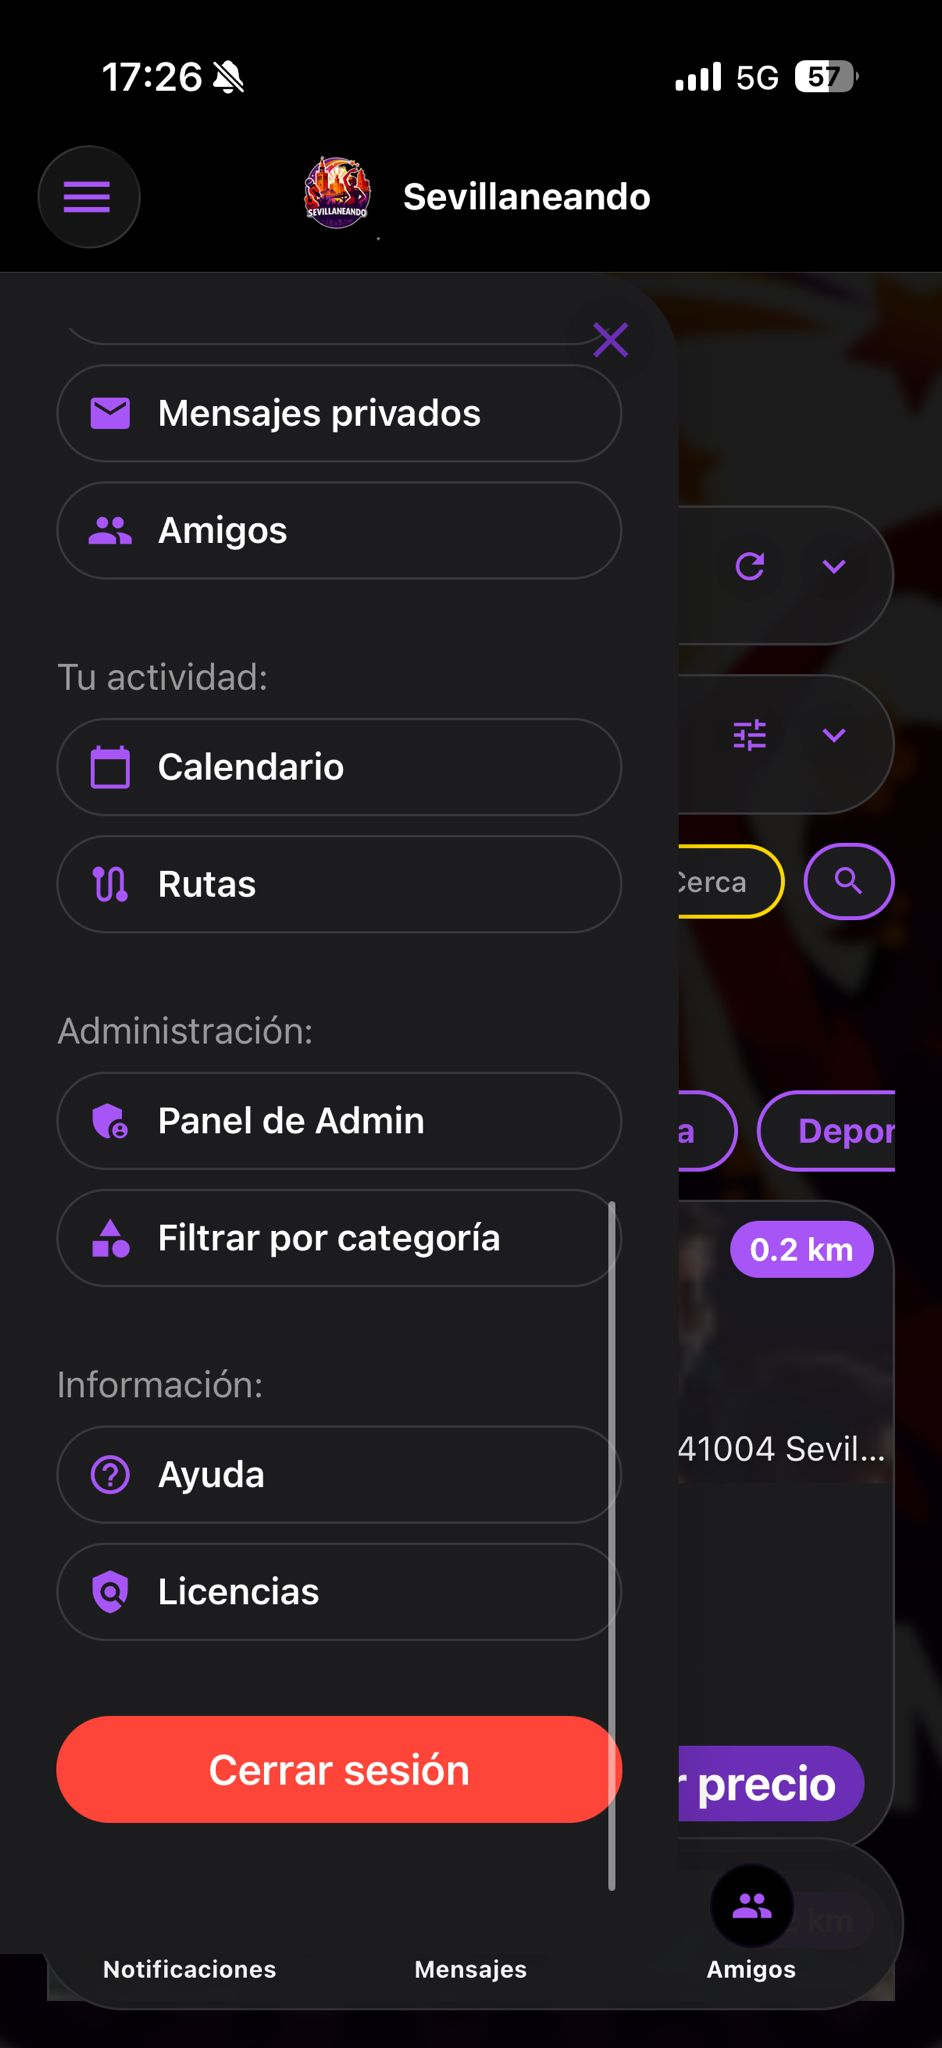
\includegraphics[width=\linewidth]{figures/paso7/menu_admin.png}
        \caption{Menú de administrador}
    \end{subfigure}
    \hspace{0.02\linewidth}
    \begin{subfigure}{0.312\linewidth}
        \centering
        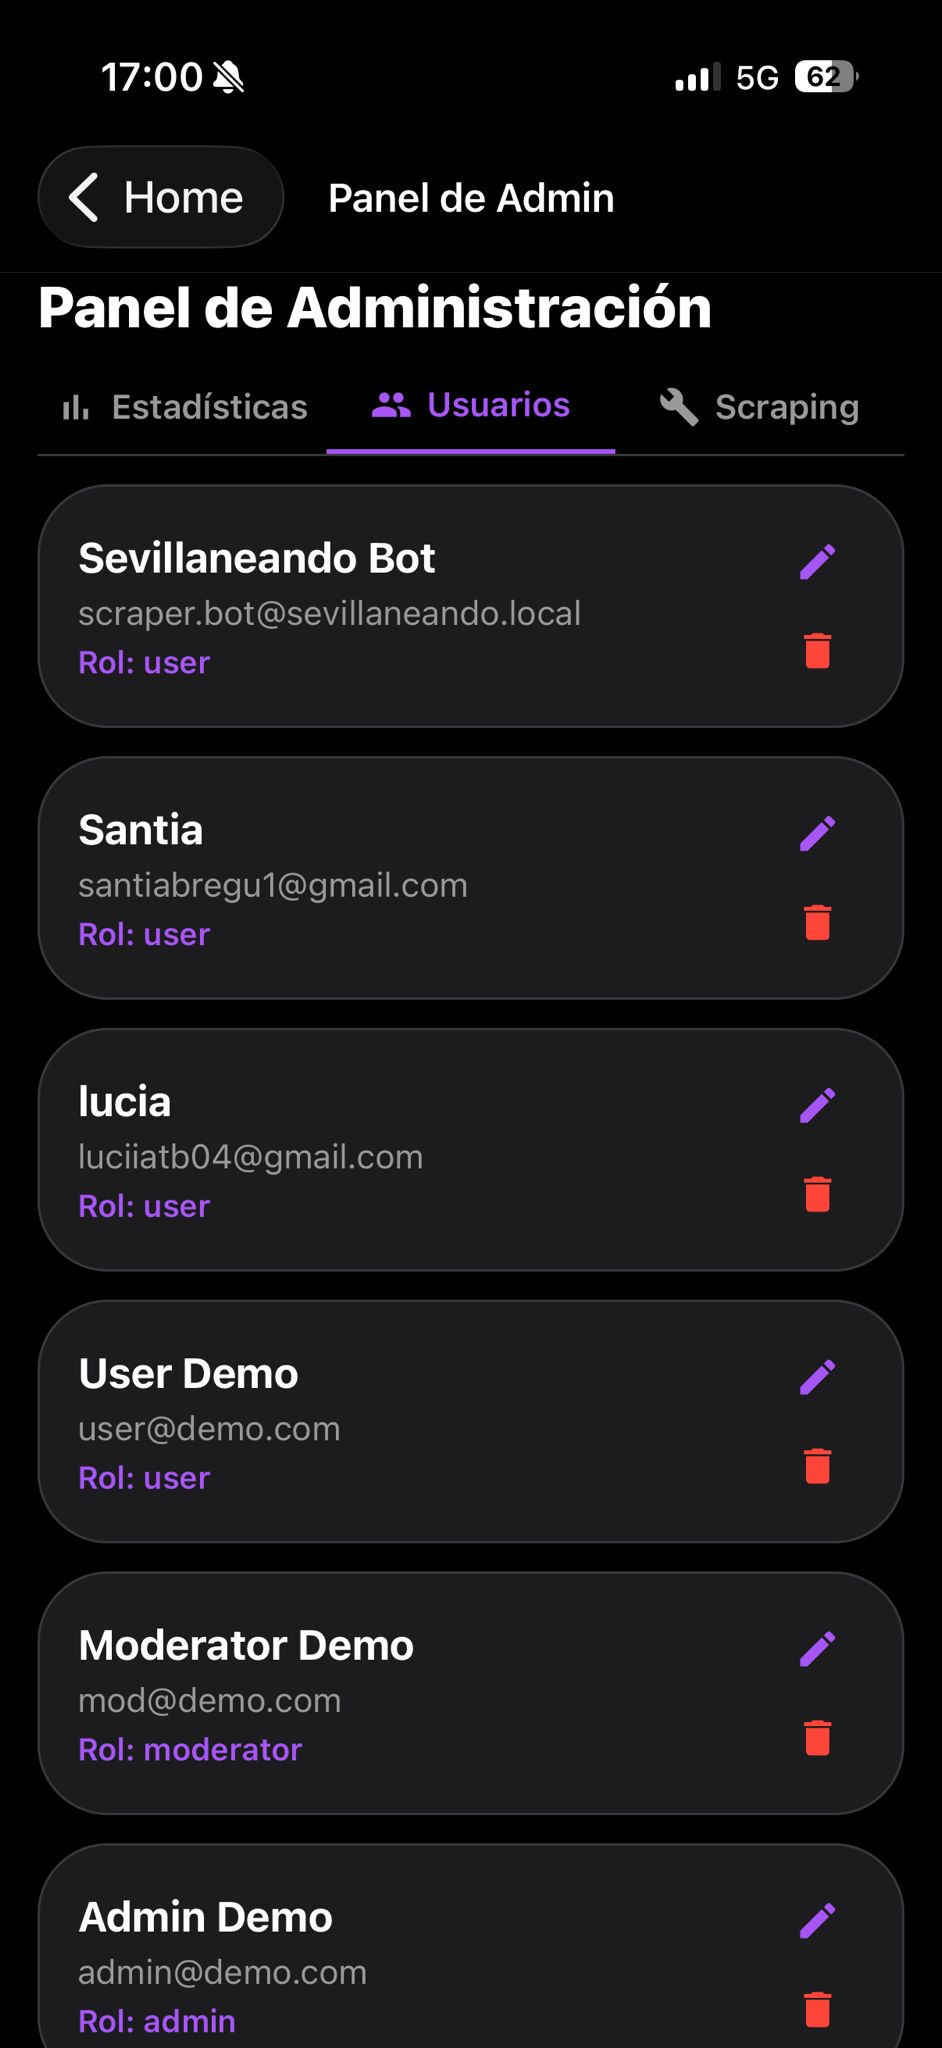
\includegraphics[width=\linewidth]{figures/paso7/panel_admin.png}
        \caption{Gestión de usuarios}
    \end{subfigure}
    \hspace{0.02\linewidth}
    \begin{subfigure}{0.31\linewidth}
        \centering
        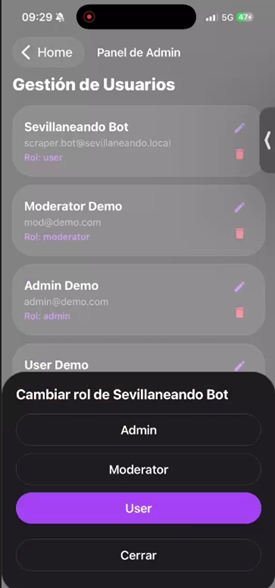
\includegraphics[width=\linewidth]{figures/paso7/edit_user.png}
        \caption{Editar usuario}
    \end{subfigure}
    \caption{Funcionalidades de administración}
\end{figure}

\begin{figure}[H]
    \centering
    \begin{subfigure}{0.35\linewidth}
        \centering
        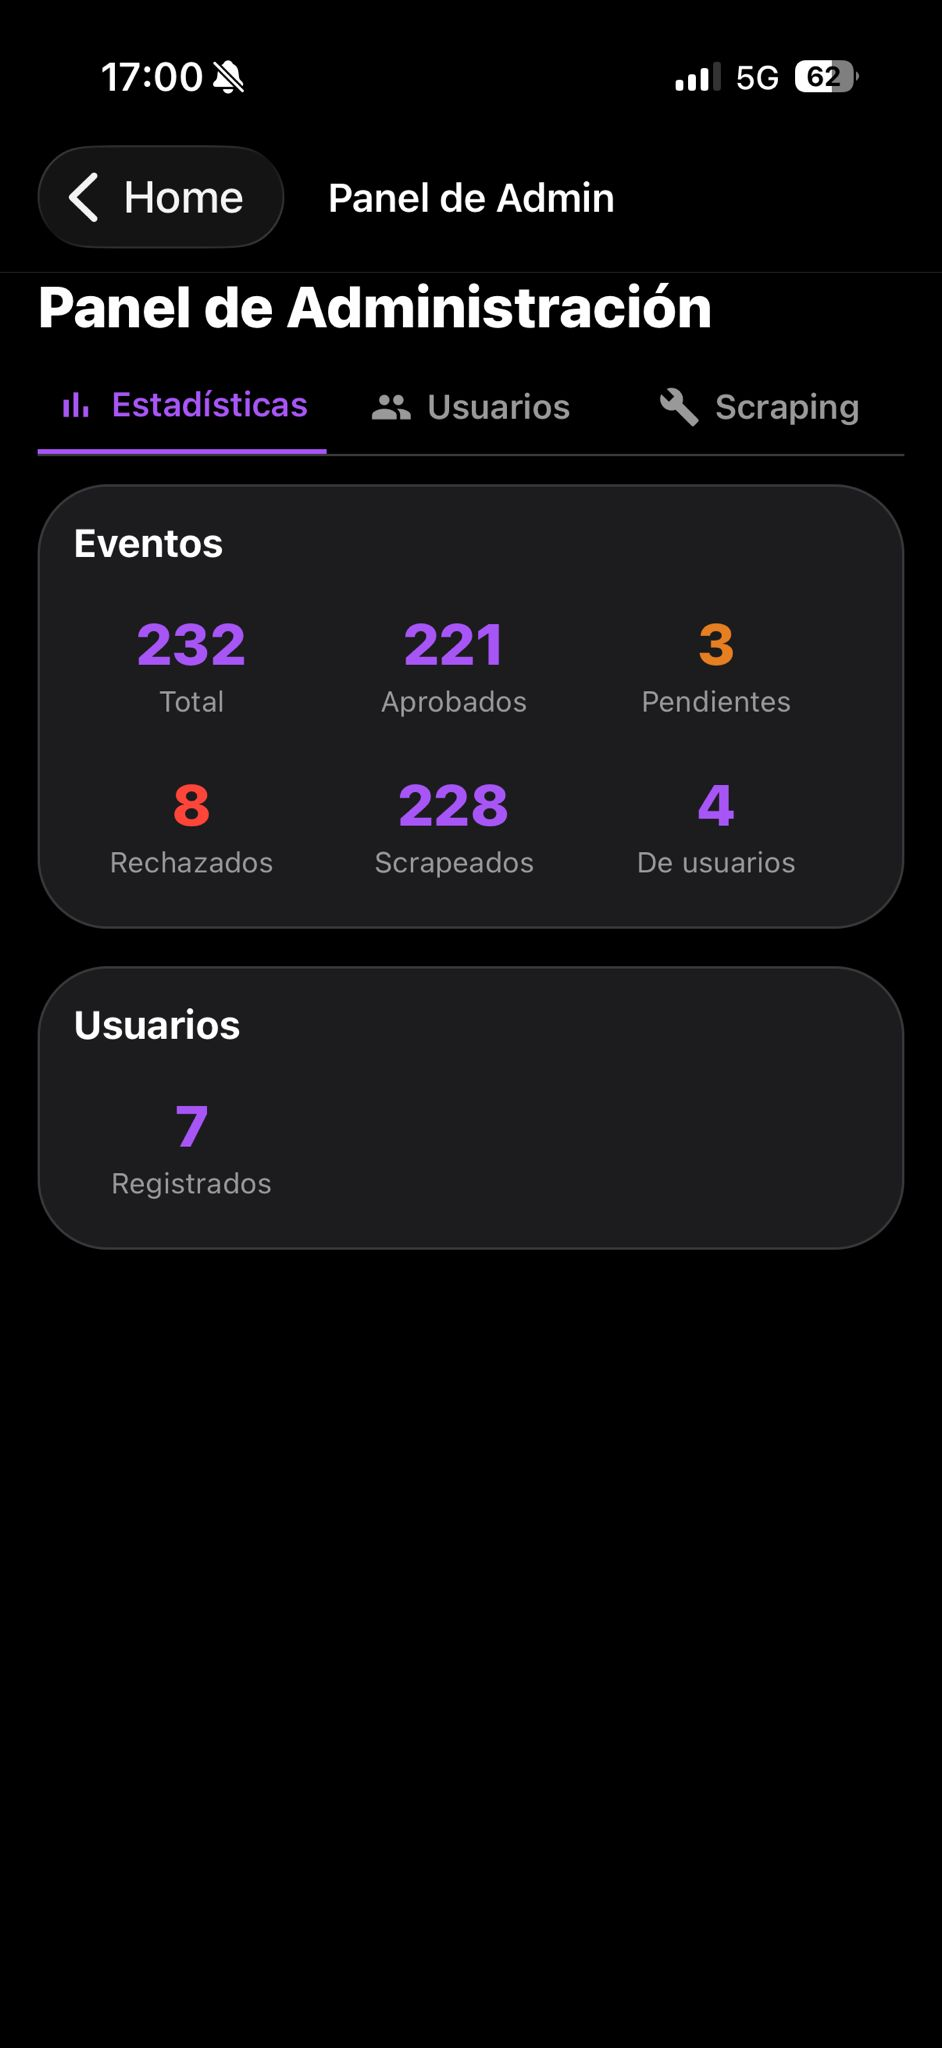
\includegraphics[width=\linewidth]{figures/paso7/panel_admin2.png}
        \caption{Estadísticas}
    \end{subfigure}
    \hspace{0.1\linewidth}
    \begin{subfigure}{0.35\linewidth}
        \centering
        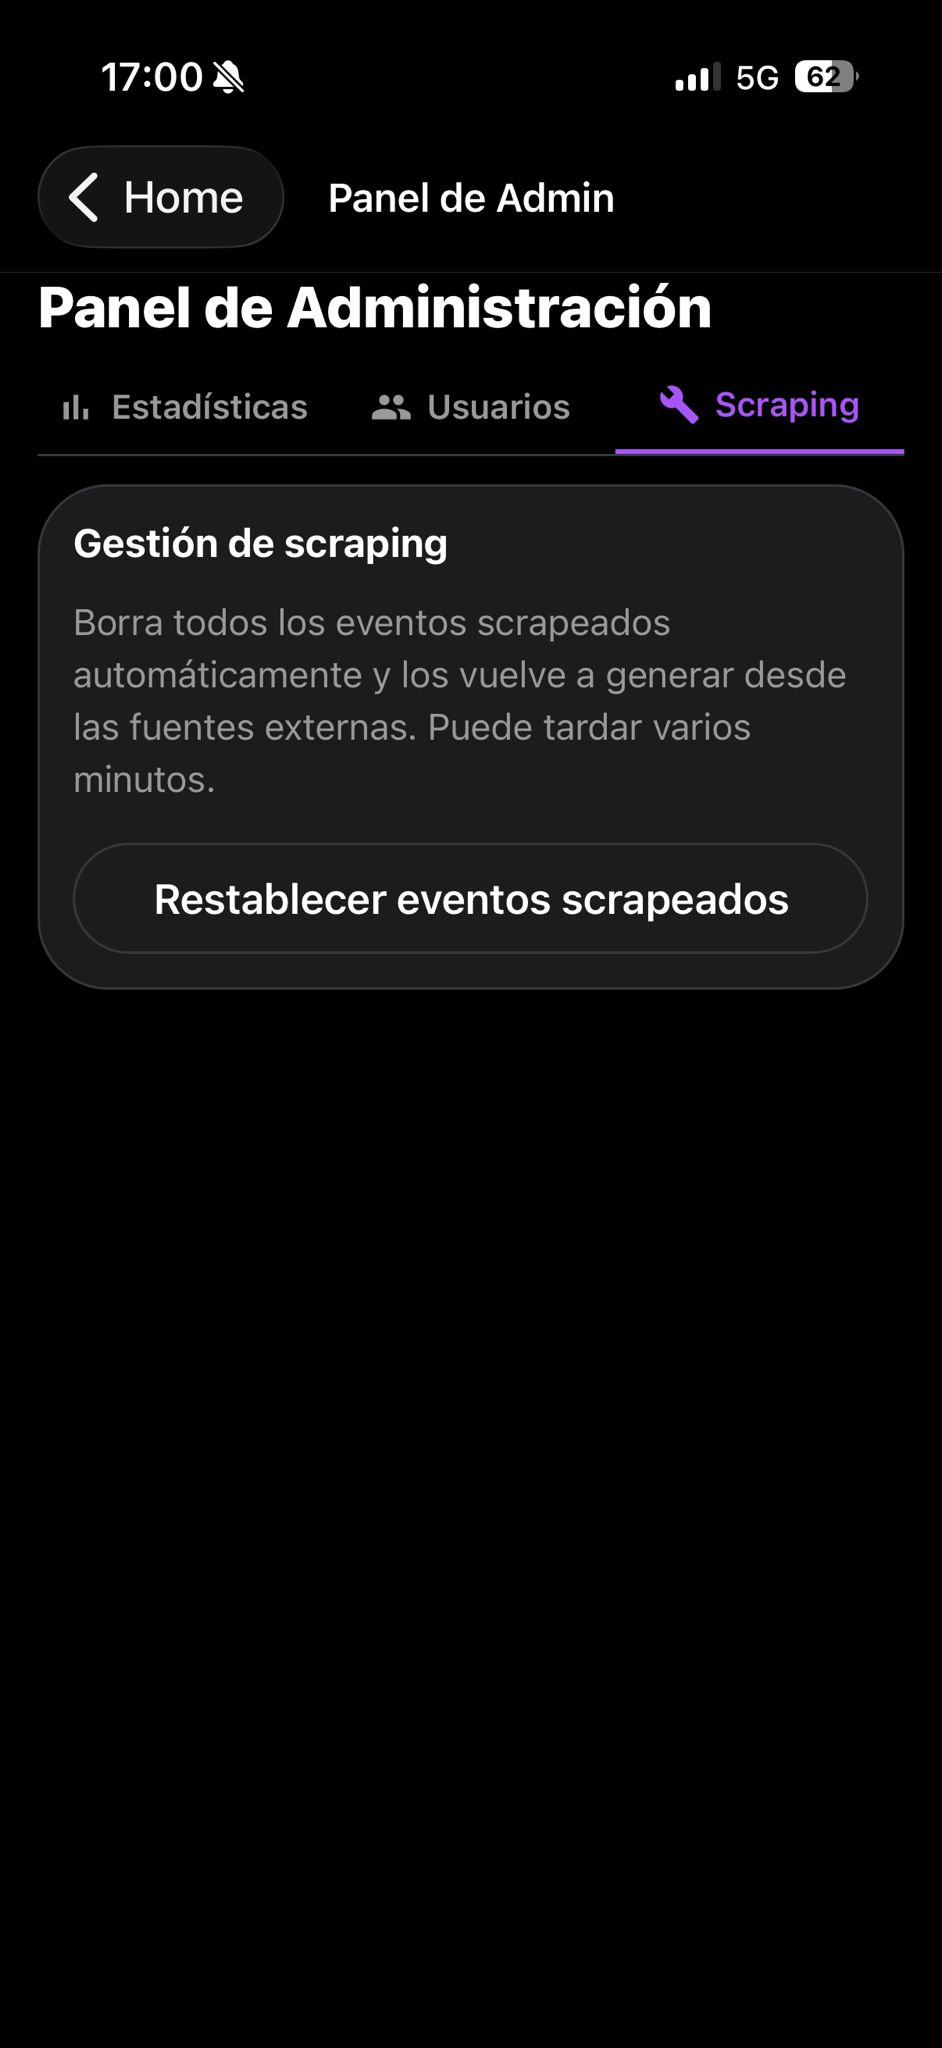
\includegraphics[width=\linewidth]{figures/paso7/panel_admin3.png}
        \caption{Scraping}
    \end{subfigure}
    \caption{Panel de estadísticas y scraping}
\end{figure}

\begin{figure}[H]
    \centering
    \begin{subfigure}{0.332\linewidth}
        \centering
        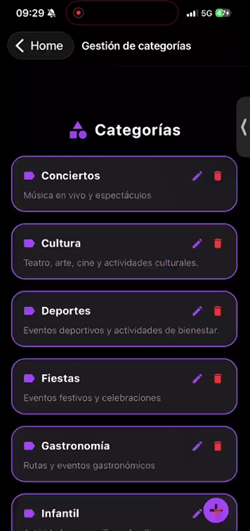
\includegraphics[width=\linewidth]{figures/paso7/gest_categ.png}
        \caption{Categorías}
    \end{subfigure}
    \hspace{0.02\linewidth}
    \begin{subfigure}{0.33\linewidth}
        \centering
        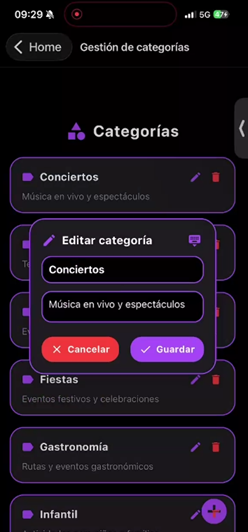
\includegraphics[width=\linewidth]{figures/paso7/edit_category.png}
        \caption{Editar categoría}
    \end{subfigure}
    \hspace{0.02\linewidth}
    \begin{subfigure}{0.328\linewidth}
        \centering
        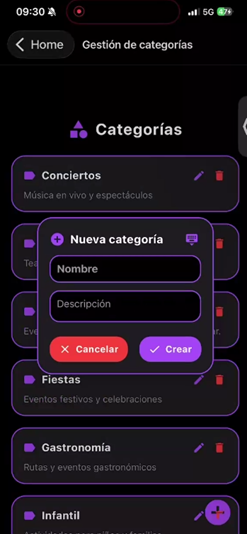
\includegraphics[width=\linewidth]{figures/paso7/crear_categ.png}
        \caption{Crear categoría}
    \end{subfigure}
    \caption{Gestión de categorías}
\end{figure}

\clearpage

\subsection{Recomendaciones y rutas recomendadas (para todos los roles)}

La página principal incorpora dos secciones personalizadas situadas por encima del listado general: \textit{Recomendaciones} y \textit{Rutas recomendadas}. Estas propuestas se generan a partir de la distancia del usuario a cada evento, sus categorías de interés, sus interacciones previas (eventos vistos, guardados, apuntados, compartidos o valorados) y la valoración media global de cada evento. Por defecto ambas secciones aparecen replegadas con un encabezado; al pulsar sobre el encabezado se despliegan y se muestran las propuestas como un carrusel horizontal de tarjetas.

En la sección \textit{Recomendaciones} se muestran inicialmente unos pocos eventos sugeridos; bajo el carrusel, el botón \textit{Ver todos} amplía la lista al conjunto completo, mientras que \textit{Ver menos} la vuelve a compactar. Al pulsar una tarjeta de evento recomendado se abre directamente la pantalla de detalle, donde el usuario puede interactuar con normalidad (apuntarse, guardar, valorar, etc.); cada interacción retroalimenta el sistema y afecta a las recomendaciones posteriores.

En la sección \textit{Rutas recomendadas} se proponen agrupaciones de varios eventos cercanos entre sí, ordenados según un recorrido óptimo. Cada tarjeta indica el título, la fecha, la puntuación media de los eventos que la integran y, en su caso, un porcentaje de calidad y el tipo de ruta. Pulsando sobre una tarjeta se abre la previsualización de la ruta con el itinerario completo. Junto a la cabecera de la sección aparece un icono de ajustes que abre una ventana emergente con la configuración de generación de rutas: el usuario puede elegir una o varias estrategias (\textit{Equilibrada}, \textit{Caminable} o \textit{Puntuación}), ajustar mediante botones \textit{+} y \textit{$-$} el número de rutas que se desean obtener y el número máximo de eventos por ruta. Tras aplicar los cambios, las rutas se recalculan automáticamente con los nuevos parámetros.

\begin{figure}[H]
    \centering
    \begin{subfigure}{0.31\linewidth}
        \centering
        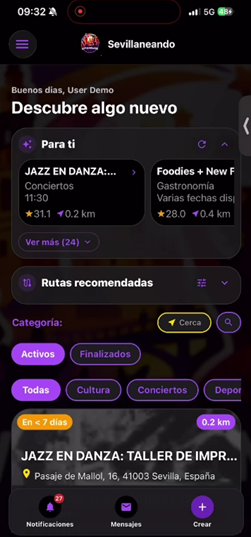
\includegraphics[width=\linewidth]{figures/paso8/recomendados.png}
        \caption{Recomendaciones}
    \end{subfigure}
    \hspace{0.01\linewidth}
    \begin{subfigure}{0.305\linewidth}
        \centering
        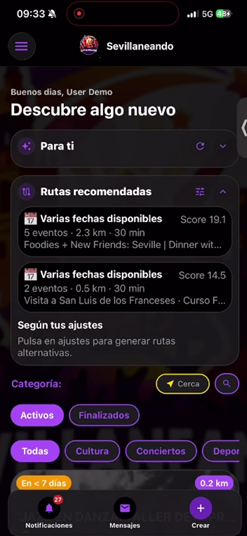
\includegraphics[width=\linewidth]{figures/paso8/rutas_recomendadas.png}
        \caption{Rutas recomendadas}
    \end{subfigure}
    \hspace{0.01\linewidth}
    \begin{subfigure}{0.302\linewidth}
        \centering
        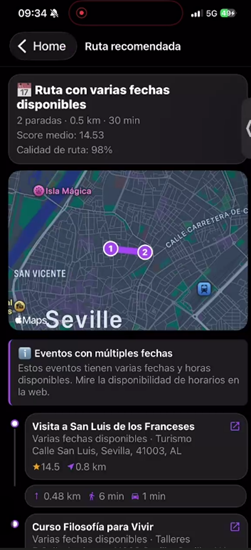
\includegraphics[width=\linewidth]{figures/paso8/detalles_ruta.png}
        \caption{Detalles de la ruta}
    \end{subfigure}
    \caption{Recomendaciones y rutas}
\end{figure}

\clearpage

\subsection{Rutas creadas por usuarios (para todos los roles)}

Además de las rutas generadas automáticamente por el sistema, la aplicación permite consultar y crear rutas manuales propuestas por la propia comunidad. Para acceder a ellas, el usuario debe abrir el menú lateral y pulsar la opción \textit{Rutas}, que muestra el listado completo de rutas existentes con su título, autor y puntuación media.

Al pulsar una ruta del listado se accede a su pantalla de detalle, donde se muestra el mapa con el recorrido completo trazado entre los puntos de interés, la lista ordenada de eventos que la integran y la sección de valoraciones. Cualquier usuario puede dejar su propia valoración, lo que contribuye a ordenar las rutas más recomendadas.

Para crear una nueva ruta, el usuario debe pulsar el botón de creación situado en la pantalla del listado. Esto abre un formulario en el que primero se introduce un título y una descripción que ayude a otros usuarios a entender la temática del recorrido. A continuación, debe indicar una duración estimada en minutos para el recorrido completo, valor que se utiliza para acotar la temporización entre paradas. La sección \textit{Eventos disponibles} muestra el catálogo de eventos del sistema, y al pulsar sobre uno este se añade a la lista \textit{Orden de visita}, donde se mantiene la secuencia de paradas en el orden de selección; al volver a pulsar sobre un evento ya seleccionado se retira de la ruta. A medida que se añaden eventos, el mapa superior actualiza los marcadores y traza la línea del recorrido entre ellos. Si dos eventos comparten exactamente las mismas coordenadas, sus marcadores se desplazan ligeramente para seguir siendo visibles.

Antes de confirmar, el usuario debe asegurarse de que todos los eventos seleccionados disponen de ubicación válida; de lo contrario, la aplicación muestra un mensaje de error al intentar guardar. Pulsando el botón final del formulario se crea la ruta y se ofrece la opción de abrir directamente su detalle, donde ya queda visible para el resto de la comunidad.

\begin{figure}[H]
    \centering
    \begin{subfigure}{0.245\linewidth}
        \centering
        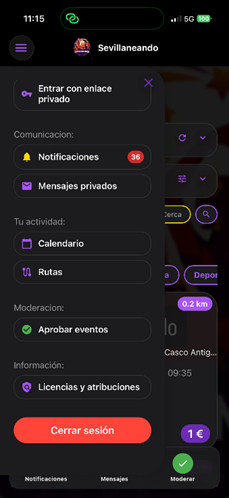
\includegraphics[width=\linewidth]{figures/paso9/menu_lateral.png}
        \caption{Menú lateral}
    \end{subfigure}
    \hspace{0.02\linewidth}
    \begin{subfigure}{0.24\linewidth}
        \centering
        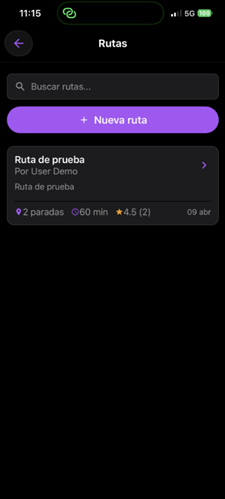
\includegraphics[width=\linewidth]{figures/paso9/rutas.png}
        \caption{Listado de rutas}
    \end{subfigure}
    \hspace{0.02\linewidth}
    \begin{subfigure}{0.245\linewidth}
        \centering
        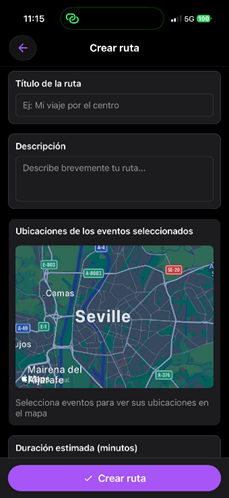
\includegraphics[width=\linewidth]{figures/paso9/crear_ruta.png}
        \caption{Crear ruta 1}
    \end{subfigure}

    \vspace{0.5cm}

    \begin{subfigure}{0.252\linewidth}
        \centering
        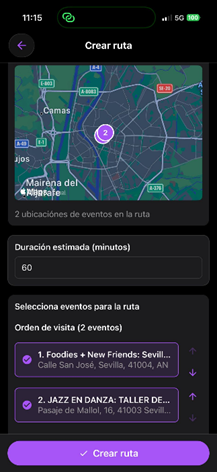
\includegraphics[width=\linewidth]{figures/paso9/crear_ruta2.png}
        \caption{Crear ruta 2}
    \end{subfigure}
    \hspace{0.02\linewidth}
    \begin{subfigure}{0.252\linewidth}
        \centering
        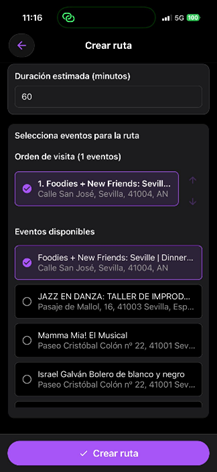
\includegraphics[width=\linewidth]{figures/paso9/crear_ruta3.png}
        \caption{Crear ruta 3}
    \end{subfigure}
    \hspace{0.02\linewidth}
    \begin{subfigure}{0.252\linewidth}
        \centering
        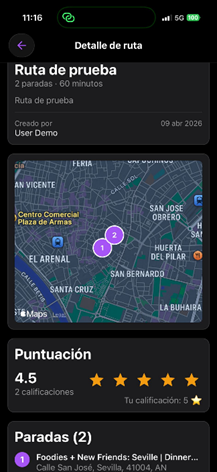
\includegraphics[width=\linewidth]{figures/paso9/detalle_ruta.png}
        \caption{Detalles de ruta}
    \end{subfigure}
    \caption{Rutas creadas por usuarios}
\end{figure}

\clearpage

\subsection{Creación de eventos (rol de usuario)}

Los usuarios pueden iniciar la creación de un evento desde el botón \textit{Crear evento} de la barra inferior de la página principal o desde el menú lateral. Al pulsarlo se abre un formulario extenso que debe recorrerse de arriba abajo. En primer lugar se introducen el título y la descripción del evento mediante dos campos de texto; la descripción admite varios párrafos. A continuación se definen la fecha de inicio y la fecha de fin pulsando los campos correspondientes, lo que abre un calendario y un selector de hora para fijar el momento exacto.

El siguiente bloque corresponde a la ubicación. El usuario puede escribir una dirección o el nombre de un lugar en el campo de búsqueda y pulsar la lupa para localizarlo automáticamente, o bien tocar directamente sobre el mapa para situar el marcador donde desee. La dirección elegida se muestra debajo del mapa. Más abajo se selecciona la categoría desde un desplegable con todas las categorías disponibles en el sistema.

El precio puede expresarse de tres formas distintas. Si se deja el campo principal vacío y los campos mínimo y máximo también, el evento se considera gratuito. Si se rellena solo el campo principal, se publica con ese precio fijo. Si se rellenan los campos \textit{Precio mínimo} y \textit{Precio máximo}, el evento mostrará un rango. La aplicación valida que el mínimo sea inferior al máximo y que no se combinen un precio fijo con un rango.

A continuación se encuentra la sección de recurrencia, marcada como opcional. Pulsando el botón de recurrencia se elige entre las opciones \textit{Diaria}, \textit{Semanal}, \textit{Quincenal} o \textit{Mensual}, y aparece un campo adicional para indicar la fecha límite hasta la que se repite el evento. Si no se desea recurrencia, basta con dejar este bloque sin tocar.

Más abajo se gestionan las imágenes del evento. El usuario puede subir varias fotos desde la galería del dispositivo, hasta un límite indicado por la aplicación. La primera imagen subida se marca por defecto como portada, pero puede cambiarse pulsando la opción \textit{Elegir como portada} sobre cualquiera de las imágenes. También es posible eliminar imágenes individualmente.

Finalmente, en la parte inferior se sitúa el interruptor \textit{Evento privado}. Si se deja desactivado, al pulsar el botón de creación el evento se envía a moderación y permanece oculto hasta su aprobación. Si se activa, el evento se publica directamente como privado sin pasar por moderación y, al terminar la creación, la aplicación abre una ventana emergente con el enlace de acceso generado para que el creador pueda copiarlo y compartirlo con sus invitados.

\bigskip

\textbf{Aspectos a tener en cuenta:}
\begin{itemize}[leftmargin=1.5em]
\item Es recomendable completar todos los campos relevantes del formulario.
\item En eventos privados se genera un enlace de acceso compartible al que se tendrá que acceder para que sea visible.
\item En eventos públicos se requiere moderación antes de ser visibles para el resto.
\end{itemize}

\begin{figure}[H]
    \centering
    \begin{subfigure}{0.35\linewidth}
        \centering
        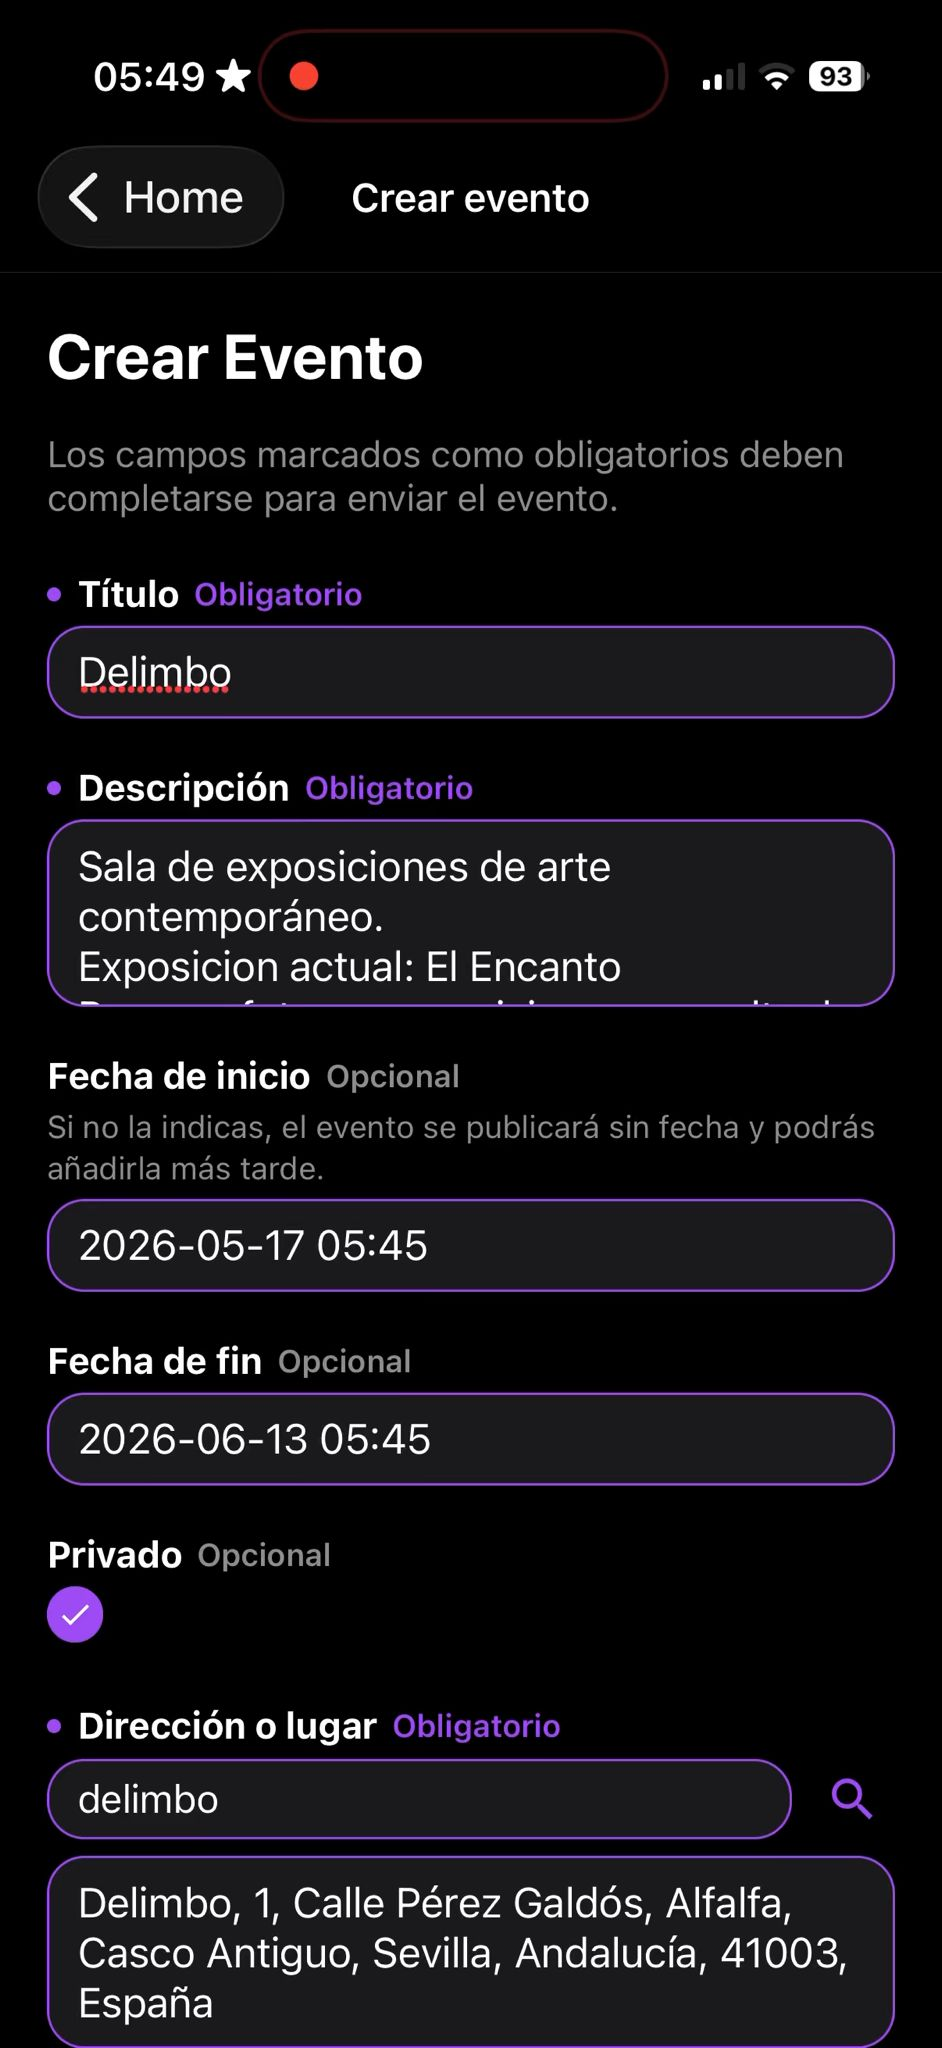
\includegraphics[width=\linewidth]{figures/paso10/crear_evento.png}
        \caption{Crear evento}
    \end{subfigure}
    \hspace{0.1\linewidth}
    \begin{subfigure}{0.356\linewidth}
        \centering
        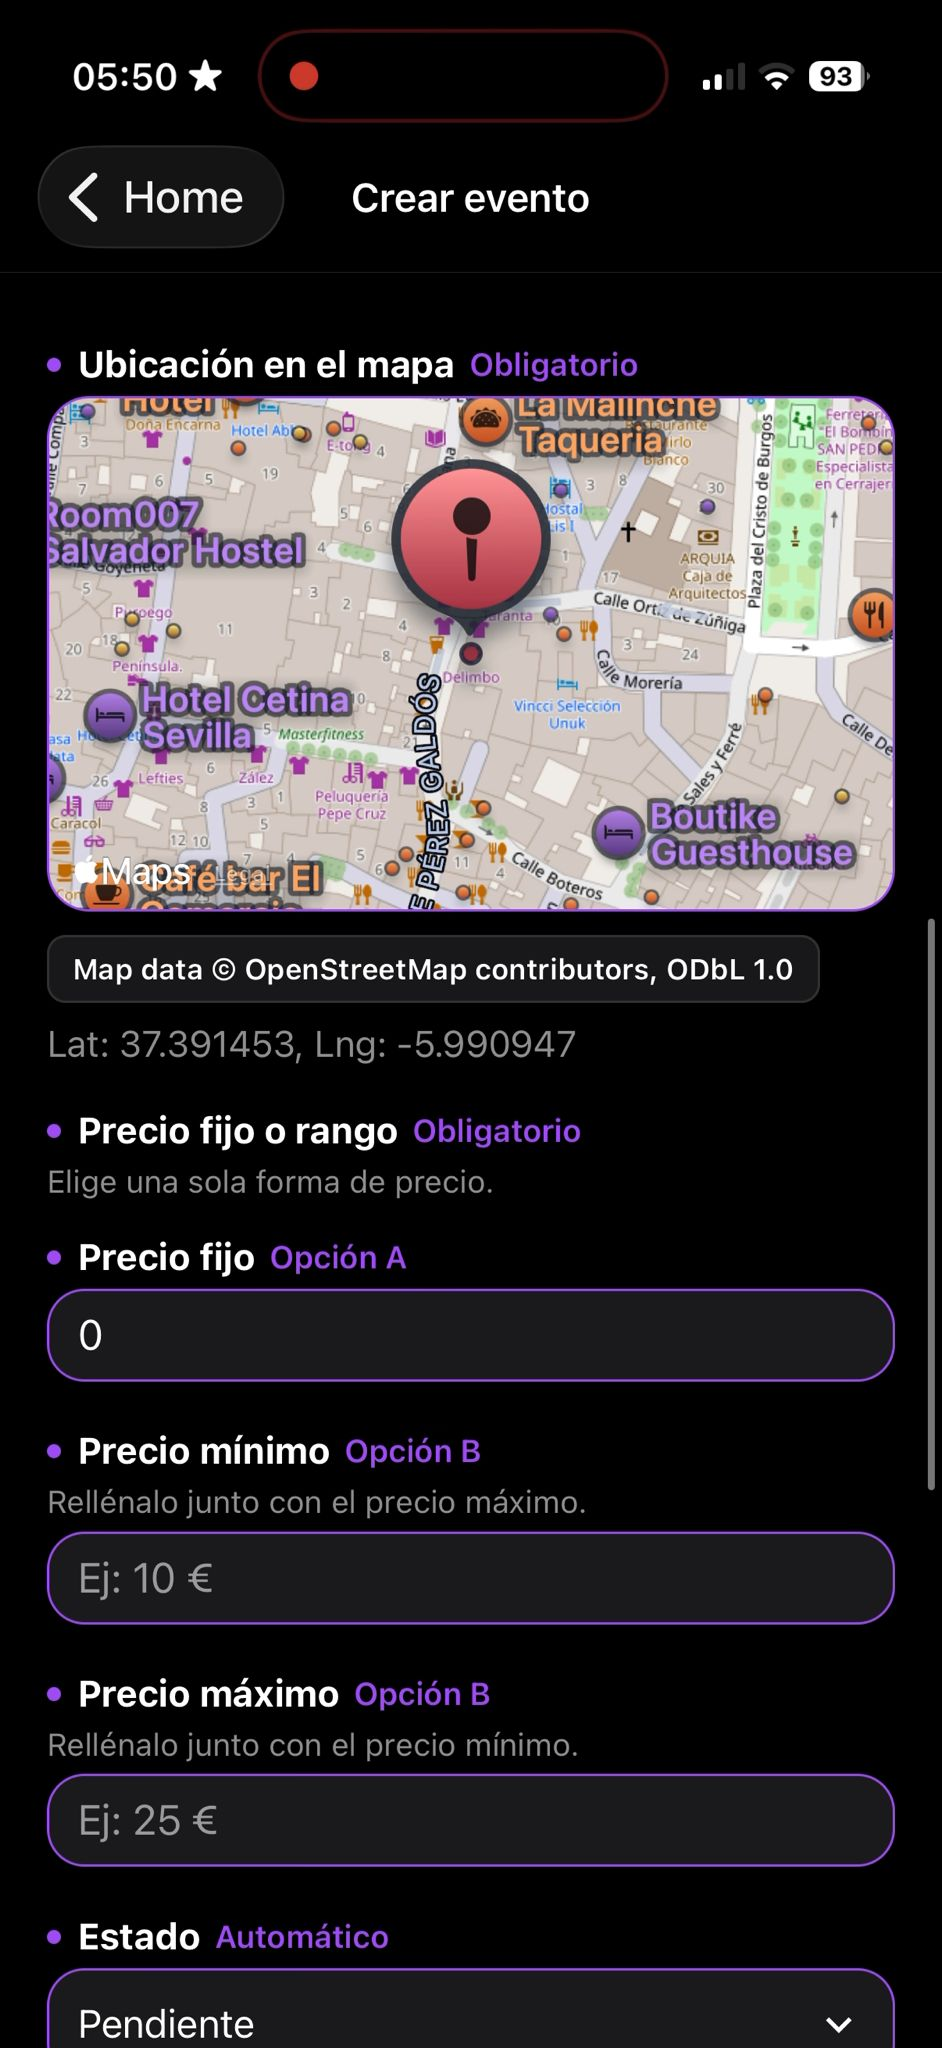
\includegraphics[width=\linewidth]{figures/paso10/crear_evento2.png}
        \caption{Crear evento 2}
    \end{subfigure}
    \caption{Creación de eventos}
\end{figure}

\begin{figure}[H]
    \centering
    \begin{subfigure}{0.35\linewidth}
        \centering
        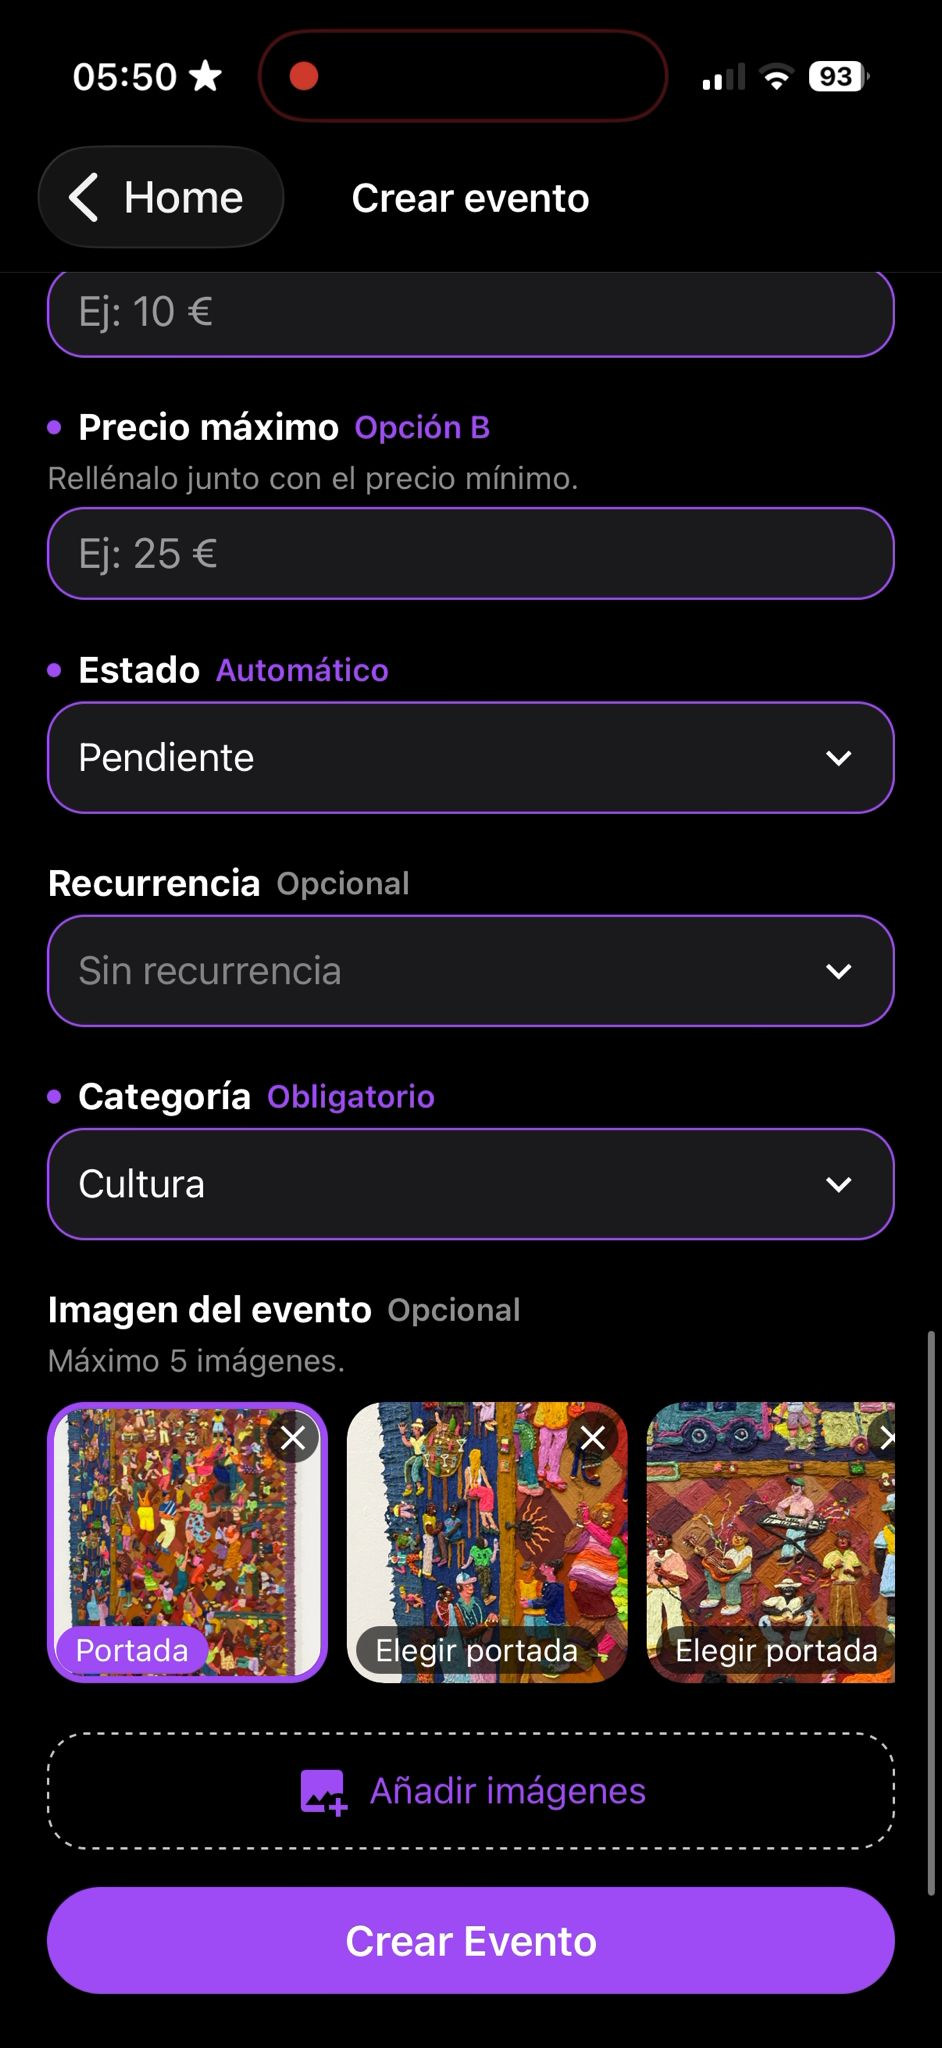
\includegraphics[width=\linewidth]{figures/paso10/crear_evento3.png}
        \caption{Crear evento 3}
    \end{subfigure}
    \hspace{0.1\linewidth}
    \begin{subfigure}{0.35\linewidth}
        \centering
        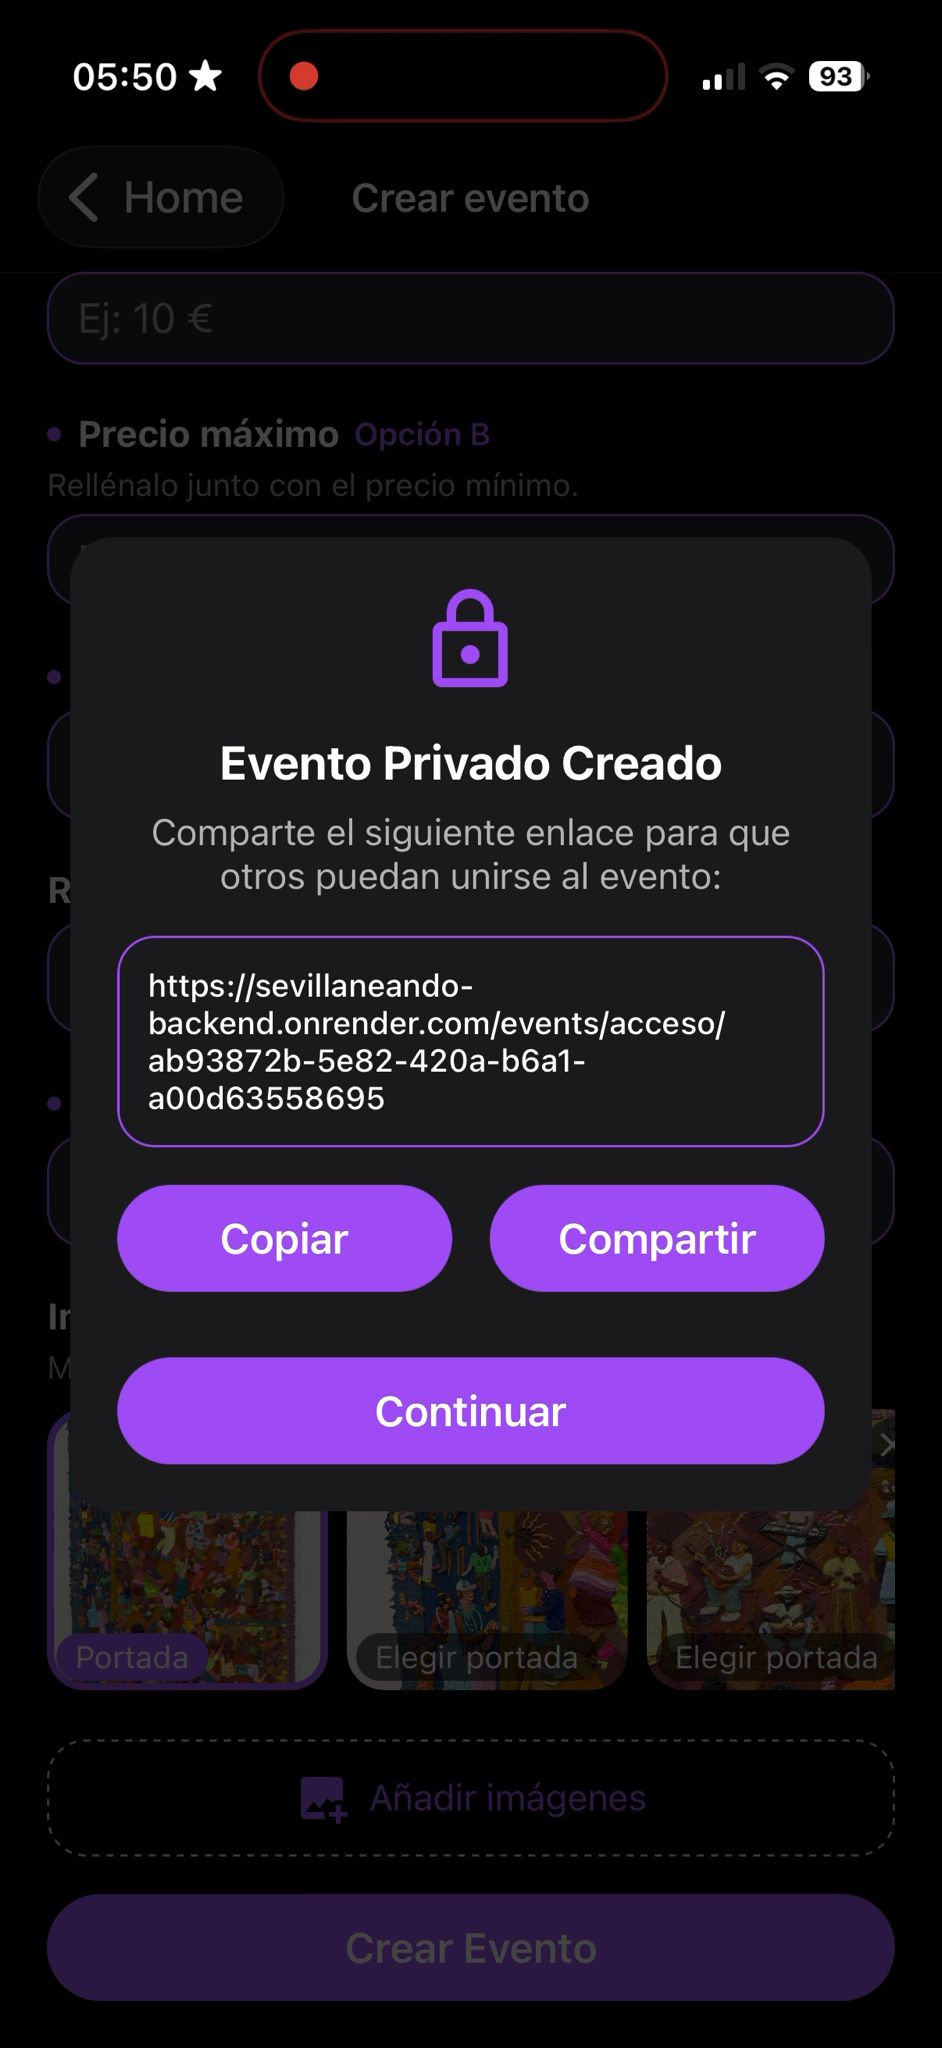
\includegraphics[width=\linewidth]{figures/paso10/evento_privado.png}
        \caption{Enlace privado}
    \end{subfigure}
    \caption{Creación de eventos }
\end{figure}

\clearpage

\subsection{Eventos privados (todos los roles)}

Los eventos privados están pensados para contextos en los que el acceso no debe ser abierto a toda la comunidad. Para participar en uno, el usuario necesita el enlace de acceso que le haya facilitado el creador. Este enlace puede recibirse a través de cualquier canal externo, como mensajería instantánea, redes sociales o correo electrónico.

Si el dispositivo tiene instalada la aplicación y se ha recibido el enlace en formato \texttt{sevillaneando://acceso/...}, basta con pulsarlo para que la aplicación se abra directamente en la pantalla del evento privado. Si el enlace es una dirección web, el usuario debe abrir manualmente la aplicación, entrar en el menú lateral y pulsar \textit{Entrar con enlace privado}; en la ventana emergente que aparece debe pegar o escribir el código de acceso recibido y pulsar \textit{Acceder}.

La aplicación carga entonces una pantalla intermedia que muestra el título del evento y dos botones, \textit{Volver} y \textit{Ver completo}. Al pulsar \textit{Ver completo} se abre la pantalla de detalle del evento con las mismas funciones que un evento público: inscripción, asistentes, valoraciones y chat. La aplicación recuerda el enlace al que se ha accedido para que el evento siga apareciendo en el listado de eventos privados del usuario aunque cierre y vuelva a abrir la aplicación. No obstante, este tipo de eventos mantiene restricciones específicas en cuanto a su difusión: el botón \textit{Compartir} solo está disponible para el creador, de modo que cualquier otro participante no puede invitar a terceros.

\begin{figure}[H]
    \centering
    \begin{subfigure}{0.30\linewidth}
        \centering
        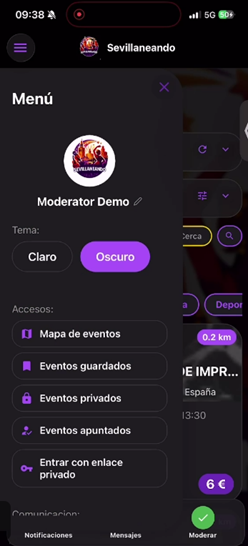
\includegraphics[width=\linewidth]{figures/paso11/menu_lateral.png}
        \caption{Menú lateral}
    \end{subfigure}
    \hspace{0.02\linewidth}
    \begin{subfigure}{0.308\linewidth}
        \centering
        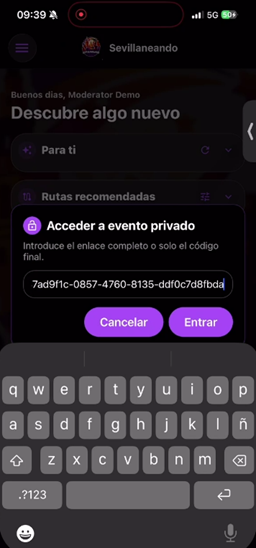
\includegraphics[width=\linewidth]{figures/paso11/evento_privado.png}
        \caption{Acceso privado}
    \end{subfigure}
    \hspace{0.02\linewidth}
    \begin{subfigure}{0.306\linewidth}
        \centering
        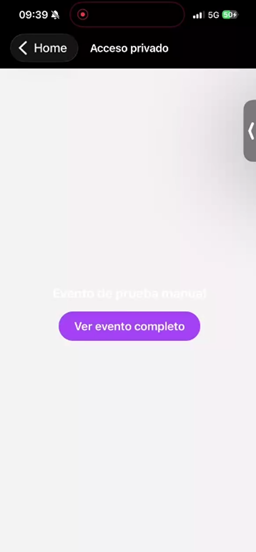
\includegraphics[width=\linewidth]{figures/paso11/evento_privado2.png}
        \caption{Ver evento privado}
    \end{subfigure}
    \caption{Acceso a evento privado}
\end{figure}

\begin{figure}[H]
    \centering
    \begin{subfigure}{0.358\linewidth}
        \centering
        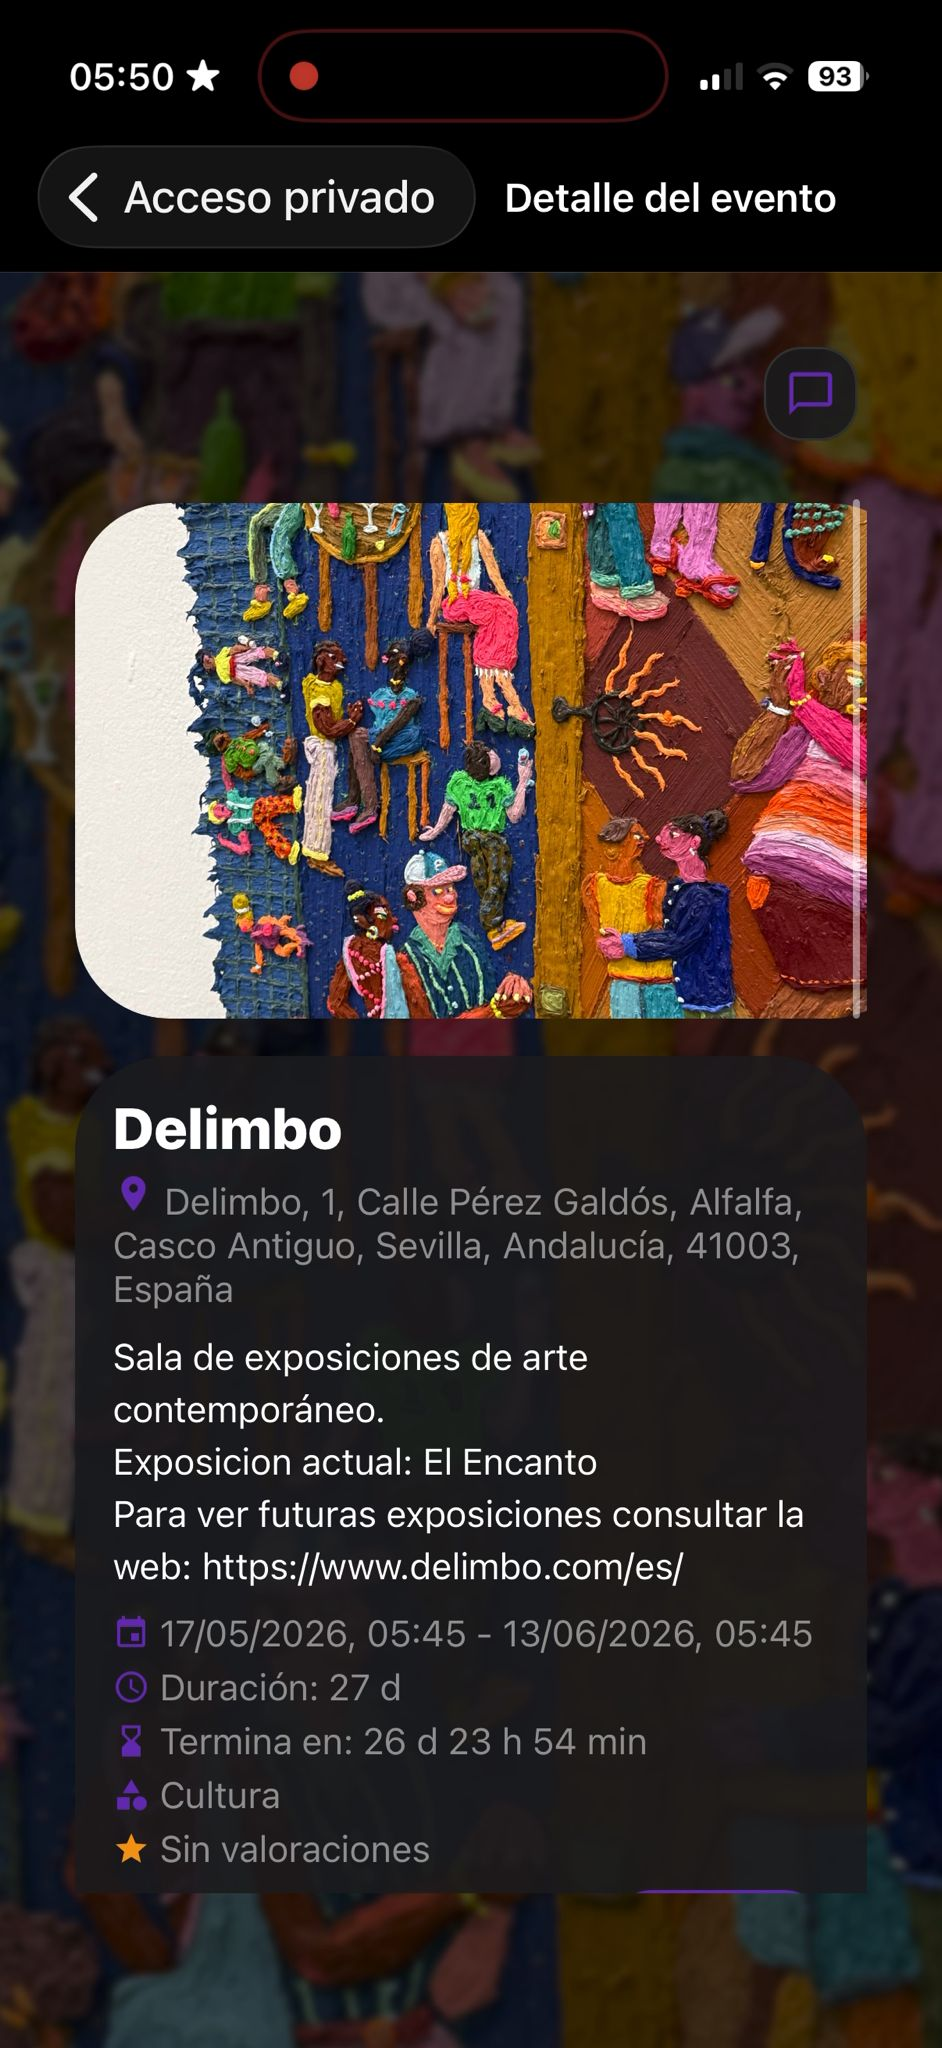
\includegraphics[width=\linewidth]{figures/paso11/detalles_event_priv.png}
        \caption{Evento privado}
    \end{subfigure}
    \hspace{0.02\linewidth}
    \begin{subfigure}{0.353\linewidth}
        \centering
        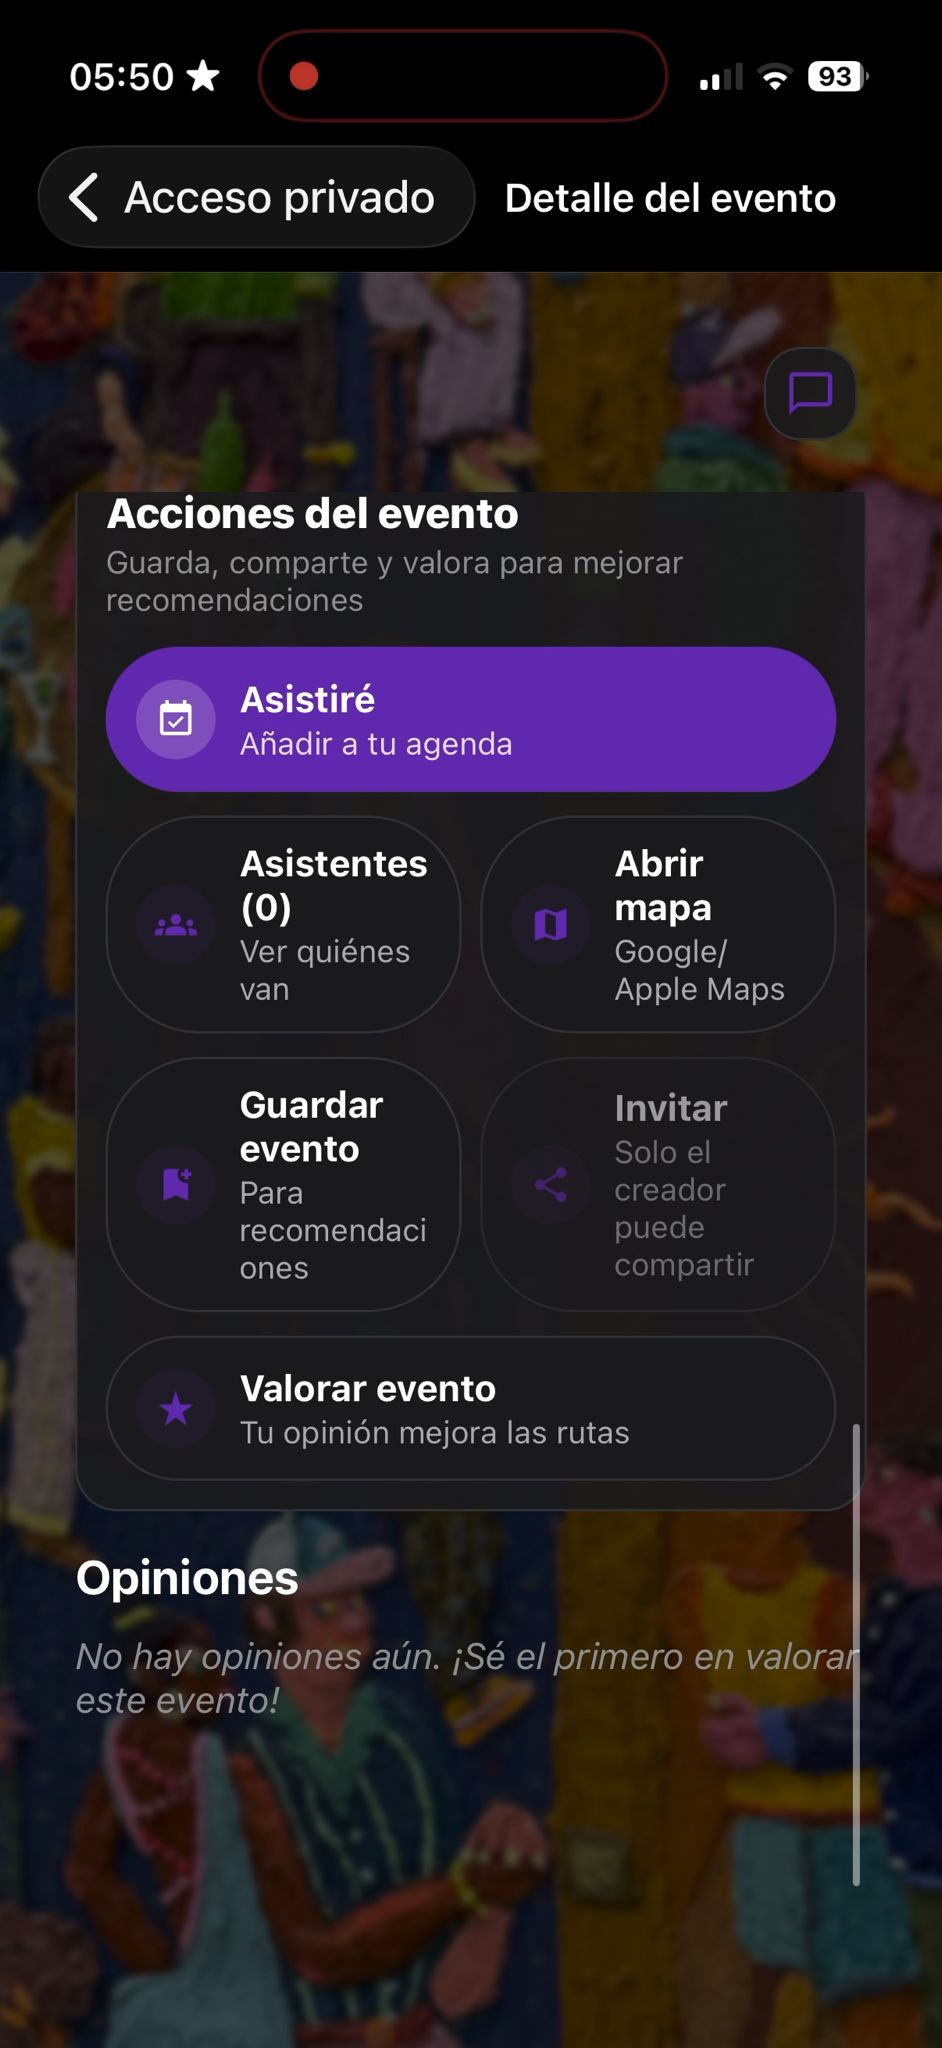
\includegraphics[width=\linewidth]{figures/paso11/det_ev_priv2.png}
        \caption{Evento privado 2}
    \end{subfigure}
    \caption{Consulta de evento privado}
\end{figure}

\clearpage

\subsection{Gestión de eventos privados (todos los roles)}

Todos los eventos privados a los que el usuario tiene acceso, ya sea como creador o como invitado, se agrupan en una misma pantalla accesible desde la opción \textit{Eventos privados} del menú lateral. En esta pantalla se combinan los eventos privados creados por el propio usuario con aquellos a los que se ha accedido mediante un enlace previamente, cuyas referencias se conservan en el dispositivo para que sigan apareciendo en visitas posteriores. Cada evento se presenta como una tarjeta con su imagen, título y fecha, y al pulsarla se abre el detalle correspondiente.

En el caso del creador, el detalle del evento privado incluye el botón \textit{Invitar} en el panel de acciones; al pulsarlo se vuelve a generar el enlace de acceso y se abre el menú nativo de compartir del dispositivo, lo que permite enviar la invitación por la vía deseada. Para los demás participantes, este botón aparece deshabilitado y la aplicación recuerda que solo el creador puede invitar a nuevos usuarios.

\begin{figure}[H]
    \centering
    \begin{subfigure}{0.35\linewidth}
        \centering
        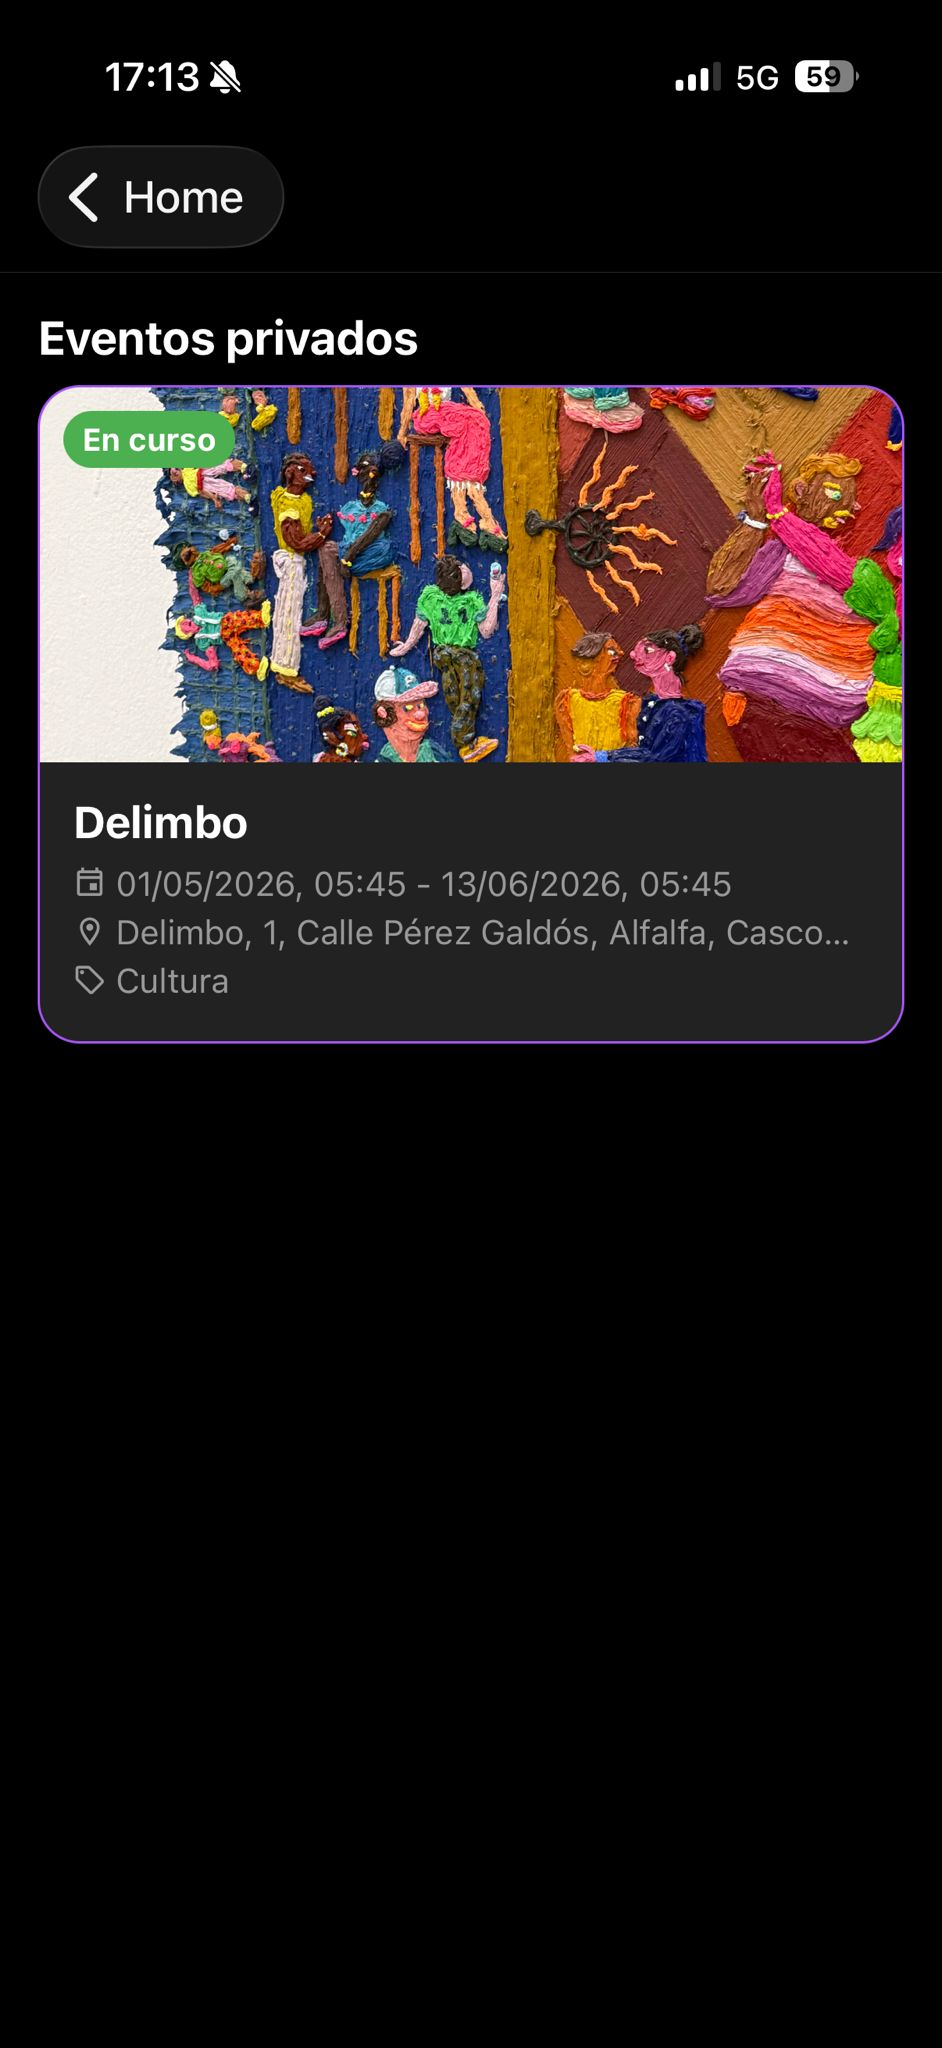
\includegraphics[width=\linewidth]{figures/paso12/eventos_priv.png}
        \caption{Eventos privados}
    \end{subfigure}
    \hspace{0.1\linewidth}
    \begin{subfigure}{0.35\linewidth}
        \centering
        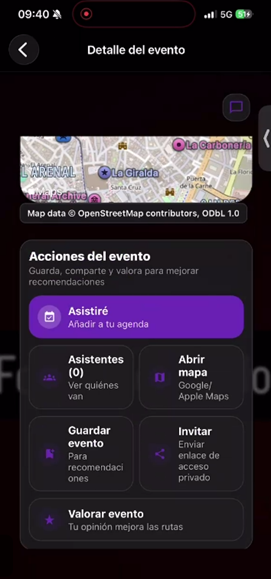
\includegraphics[width=\linewidth]{figures/paso12/det_event_priv.png}
        \caption{Evento privado}
    \end{subfigure}
    \caption{Gestión de eventos privados}
\end{figure}

\clearpage

\subsection{Mis eventos (rol de usuario)}

La sección \textit{Mis eventos}, accesible desde el menú lateral, reúne todos los eventos que el usuario ha creado. La pantalla muestra los eventos privados, los públicos ya aprobados y los públicos rechazados; los eventos públicos pendientes de moderación no aparecen en este listado, pero la propia pantalla lo recuerda mediante un aviso superior que indica cuántos eventos están actualmente esperando aprobación.

Cada evento se presenta como una tarjeta con la imagen, el título, la fecha y un indicador del estado. Al pulsar una tarjeta se accede a la pantalla de edición del evento, donde aparecen los mismos campos que en la pantalla de creación con los valores actuales precargados. El usuario puede modificar cualquier dato (título, descripción, fechas, ubicación, categoría, precio, recurrencia o imágenes) y guardar los cambios pulsando el botón principal. La propia pantalla de edición incluye, en su parte inferior, un botón rojo para eliminar el evento de forma definitiva, que requiere confirmación.

El comportamiento tras la edición depende del tipo de evento y del cambio realizado. Si se edita un evento privado, este sigue siendo visible para los participantes que ya tenían el enlace y aparece actualizado tanto para ellos como en \textit{Mis eventos}. Si un evento público se modifica, vuelve a moderación y deja temporalmente de aparecer en el listado general hasta su nueva aprobación. Si se cambia un evento de público a privado, deja de ser visible para todos los usuarios excepto en \textit{Mis eventos}, y el acceso queda restringido al enlace privado. Si se cambia de privado a público, el evento se envía a moderación, deja de ser visible mediante el enlace anterior y solo volverá a publicarse de forma general si se aprueba.
\bigskip

\textbf{Aspectos a tener en cuenta:}
\begin{itemize}[leftmargin=1.5em]

\item Cuando se edita un evento privado se mantiene visible para participantes que accedieron mediante el enlace privado y en \textit{Mis eventos}.
\item Cuando un evento pasa de público a privado deja de ser visible para todos pero se mantiene visible en \textit{Mis eventos}. Para que sea visible habría que acceder mediante el enlace privado.
\item Cuando un evento pasa de privado a público se va a moderación, deja de ser visible para las personas que habían accedido mediante el enlace y pasaría a ser visible para todos si se aprueba.
\item Cuando se edita un evento público vuelve a moderación antes de mostrarse de nuevo en el listado general.
\item Desde la pantalla de edición puede eliminarse el evento definitivamente mediante el botón correspondiente.
\end{itemize}

\begin{figure}[H]
    \centering
    \begin{subfigure}{0.31\linewidth}
        \centering
        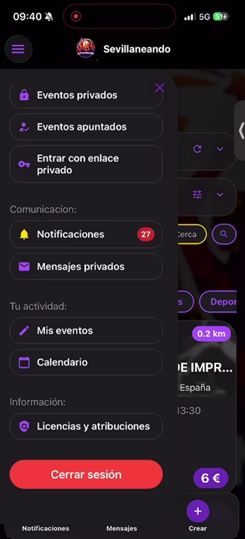
\includegraphics[width=\linewidth]{figures/paso13/menu_lateral.png}
        \caption{Menú lateral}
    \end{subfigure}
    \hspace{0.01\linewidth}
    \begin{subfigure}{0.31\linewidth}
        \centering
        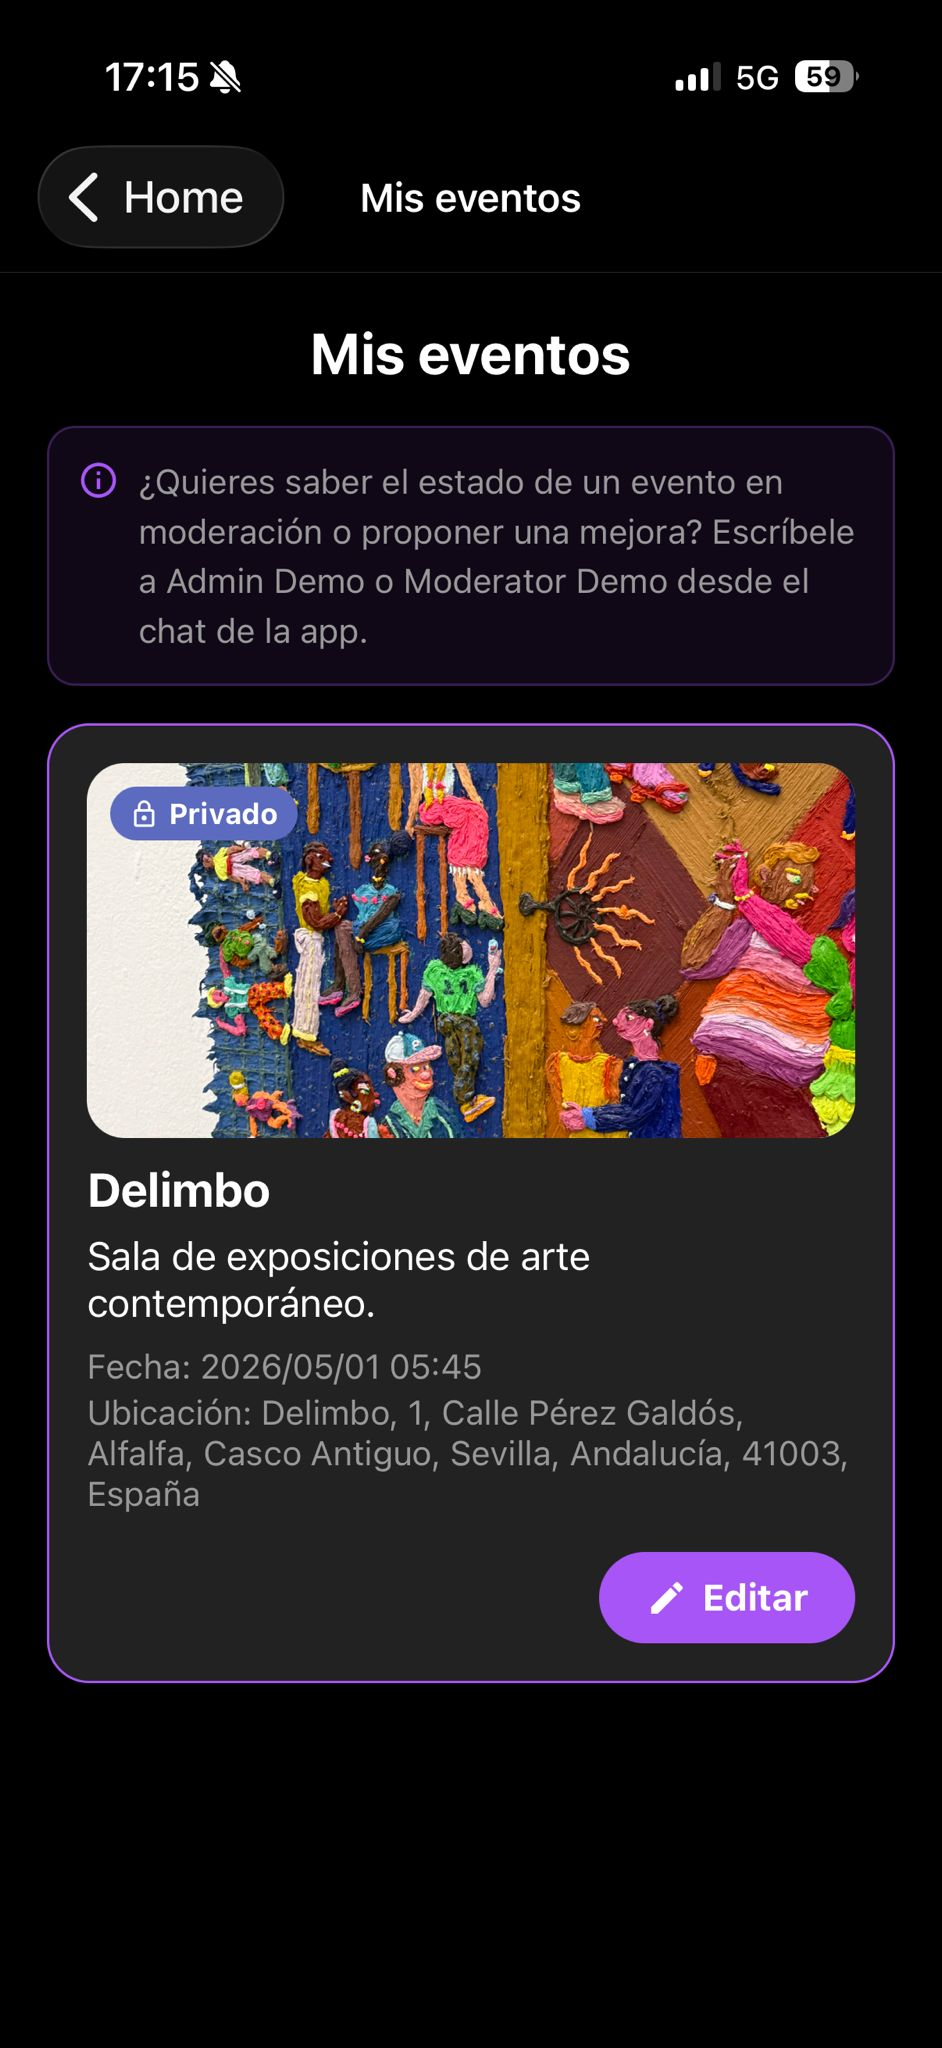
\includegraphics[width=\linewidth]{figures/paso13/mis_eventos.png}
        \caption{Mis eventos}
    \end{subfigure}
    \hspace{0.01\linewidth}
    \begin{subfigure}{0.31\linewidth}
        \centering
        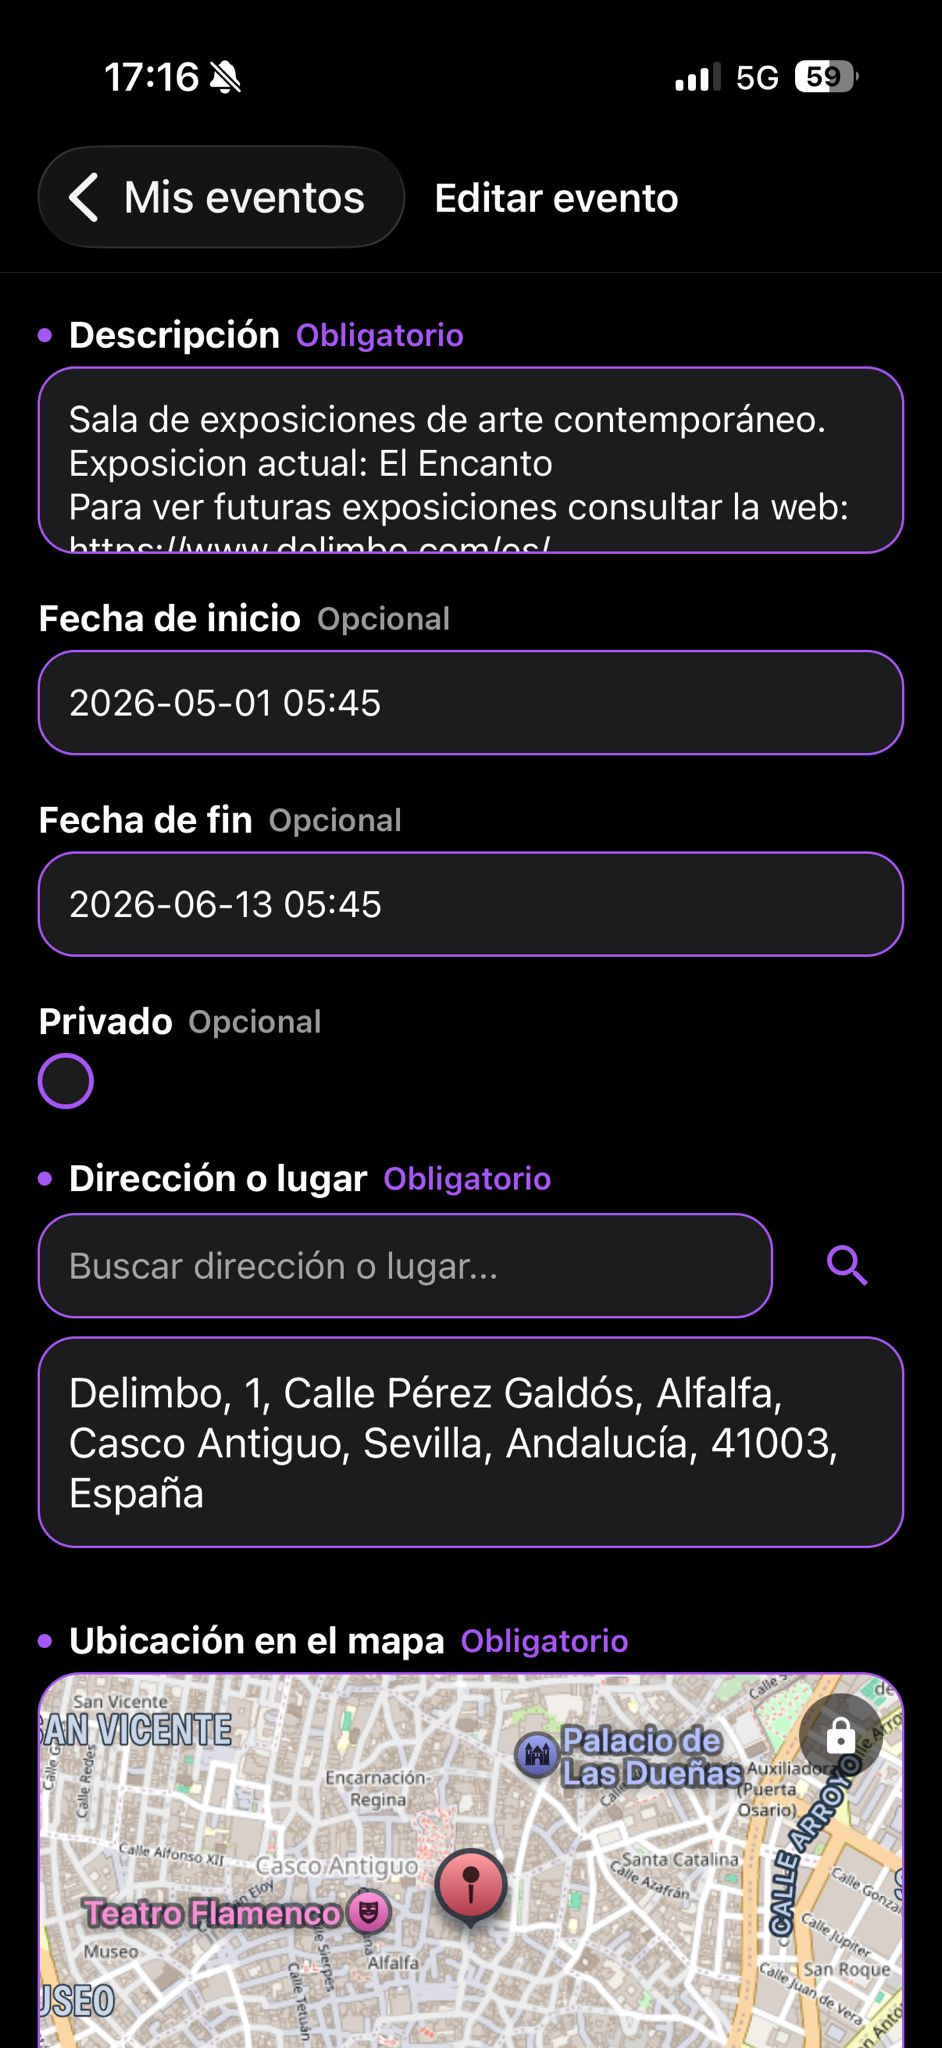
\includegraphics[width=\linewidth]{figures/paso13/editar_evento.png}
        \caption{Editar evento}
    \end{subfigure}
    \hspace{0.01\linewidth}
    \begin{subfigure}{0.31\linewidth}
        \centering
        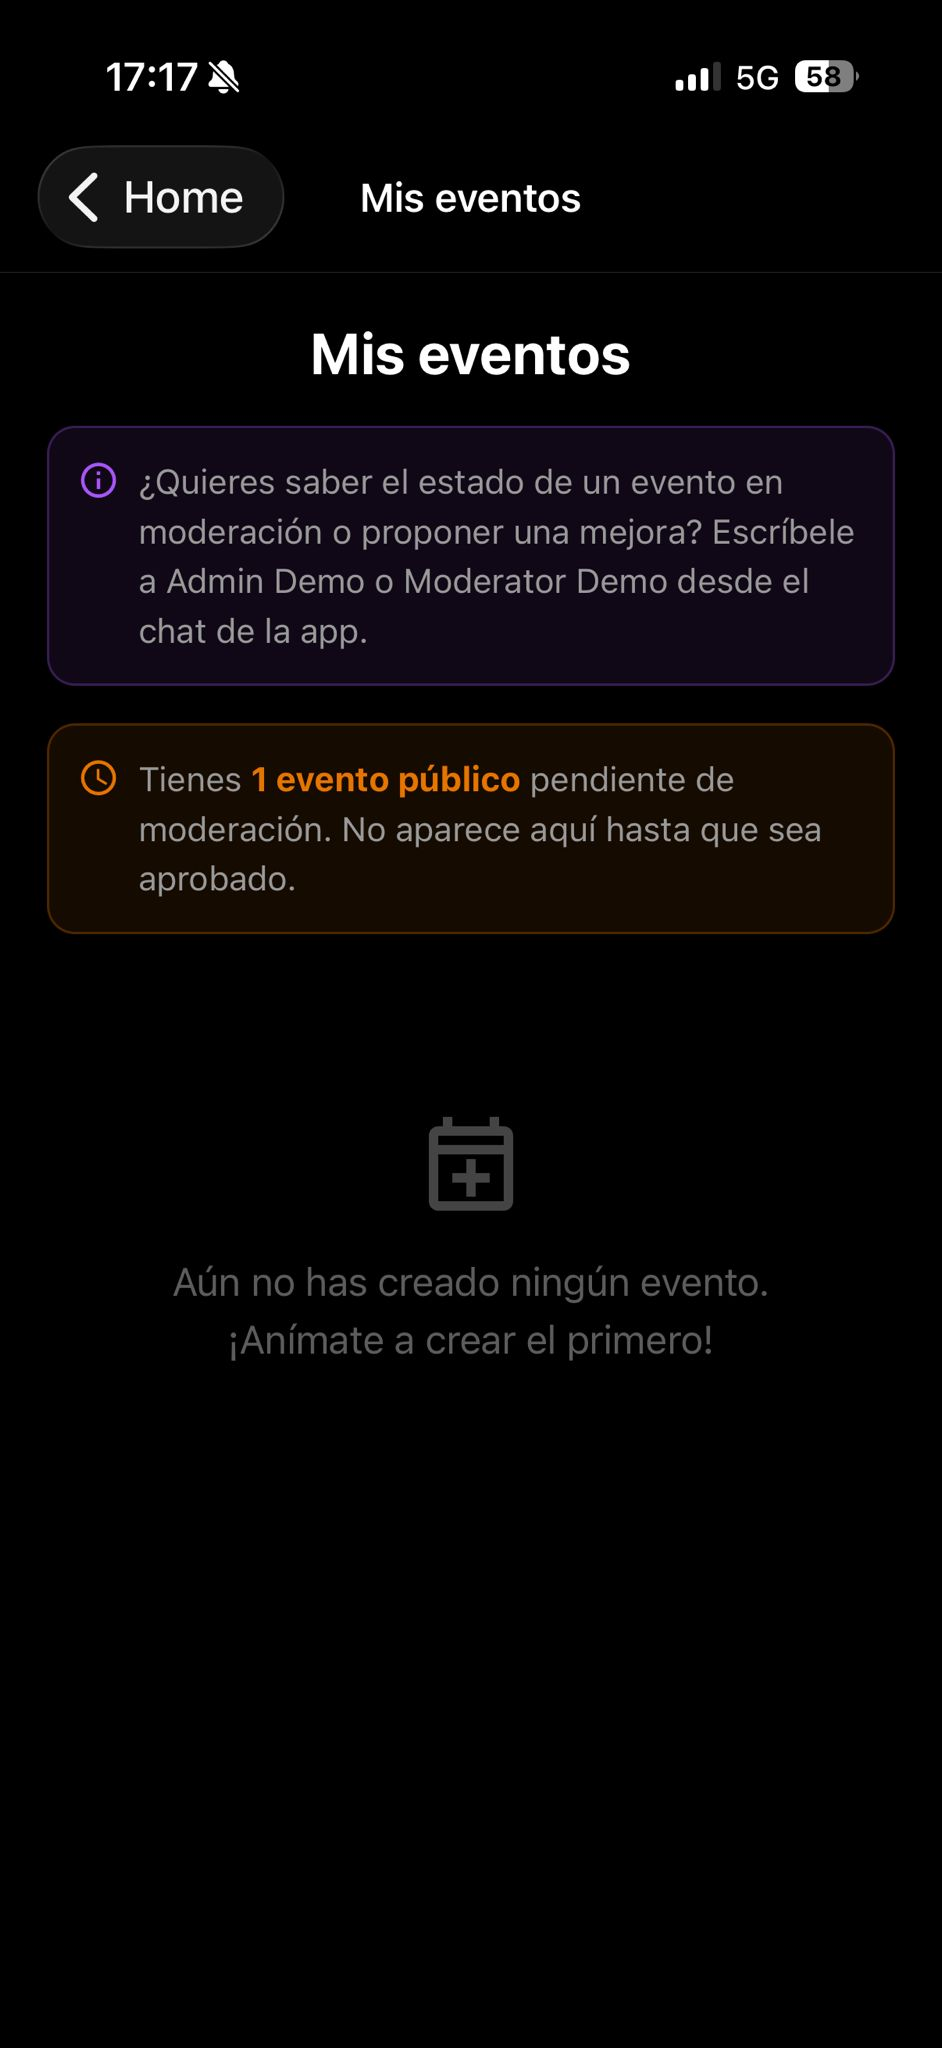
\includegraphics[width=\linewidth]{figures/paso13/evento_moderacion.png}
        \caption{Evento en moderación}
    \end{subfigure}
    \caption{Eventos creados por el usuario}
\end{figure}

\clearpage

\subsection{Moderación (rol de moderador)}

Los usuarios con rol de moderador disponen, en la barra inferior de la página principal y en el menú lateral, de un acceso adicional a la pantalla \textit{Moderación}. Esta pantalla se organiza en dos pestañas que pueden alternarse pulsando su título: \textit{Pendientes} y \textit{Públicos aprobados}.

En la pestaña \textit{Pendientes} se muestran los eventos públicos que aún no han sido validados, ordenados por fecha de creación. Cada tarjeta incluye la imagen, el título, las fechas, la categoría y el creador. Al pulsar la tarjeta se abre una pantalla de revisión del evento donde el moderador puede consultar todos los datos y, si es necesario, editarlos antes de tomar una decisión. En esa misma pantalla aparecen los botones \textit{Aprobar} y \textit{Rechazar}: el primero publica el evento de manera inmediata y lo hace visible para toda la comunidad; el segundo lo marca como rechazado y notifica al creador. Tras cualquiera de las dos acciones la lista de pendientes se actualiza automáticamente.

La pestaña \textit{Públicos aprobados} muestra todos los eventos públicos que ya están publicados. El moderador puede pulsar sobre cualquiera de ellos para abrir la pantalla de edición y modificar los datos del evento, e incluso eliminarlo en caso de que sea necesario. Esta acción no afecta a los eventos privados de la plataforma, que quedan fuera del alcance de moderación.

\bigskip

\textbf{Credenciales de prueba:}
\begin{itemize}[leftmargin=1.5em]
\item Email: \texttt{mod@demo.com}
\item Contraseña: \texttt{moderator}
\end{itemize}

\begin{figure}[H]
    \centering
    \begin{subfigure}{0.31\linewidth}
        \centering
        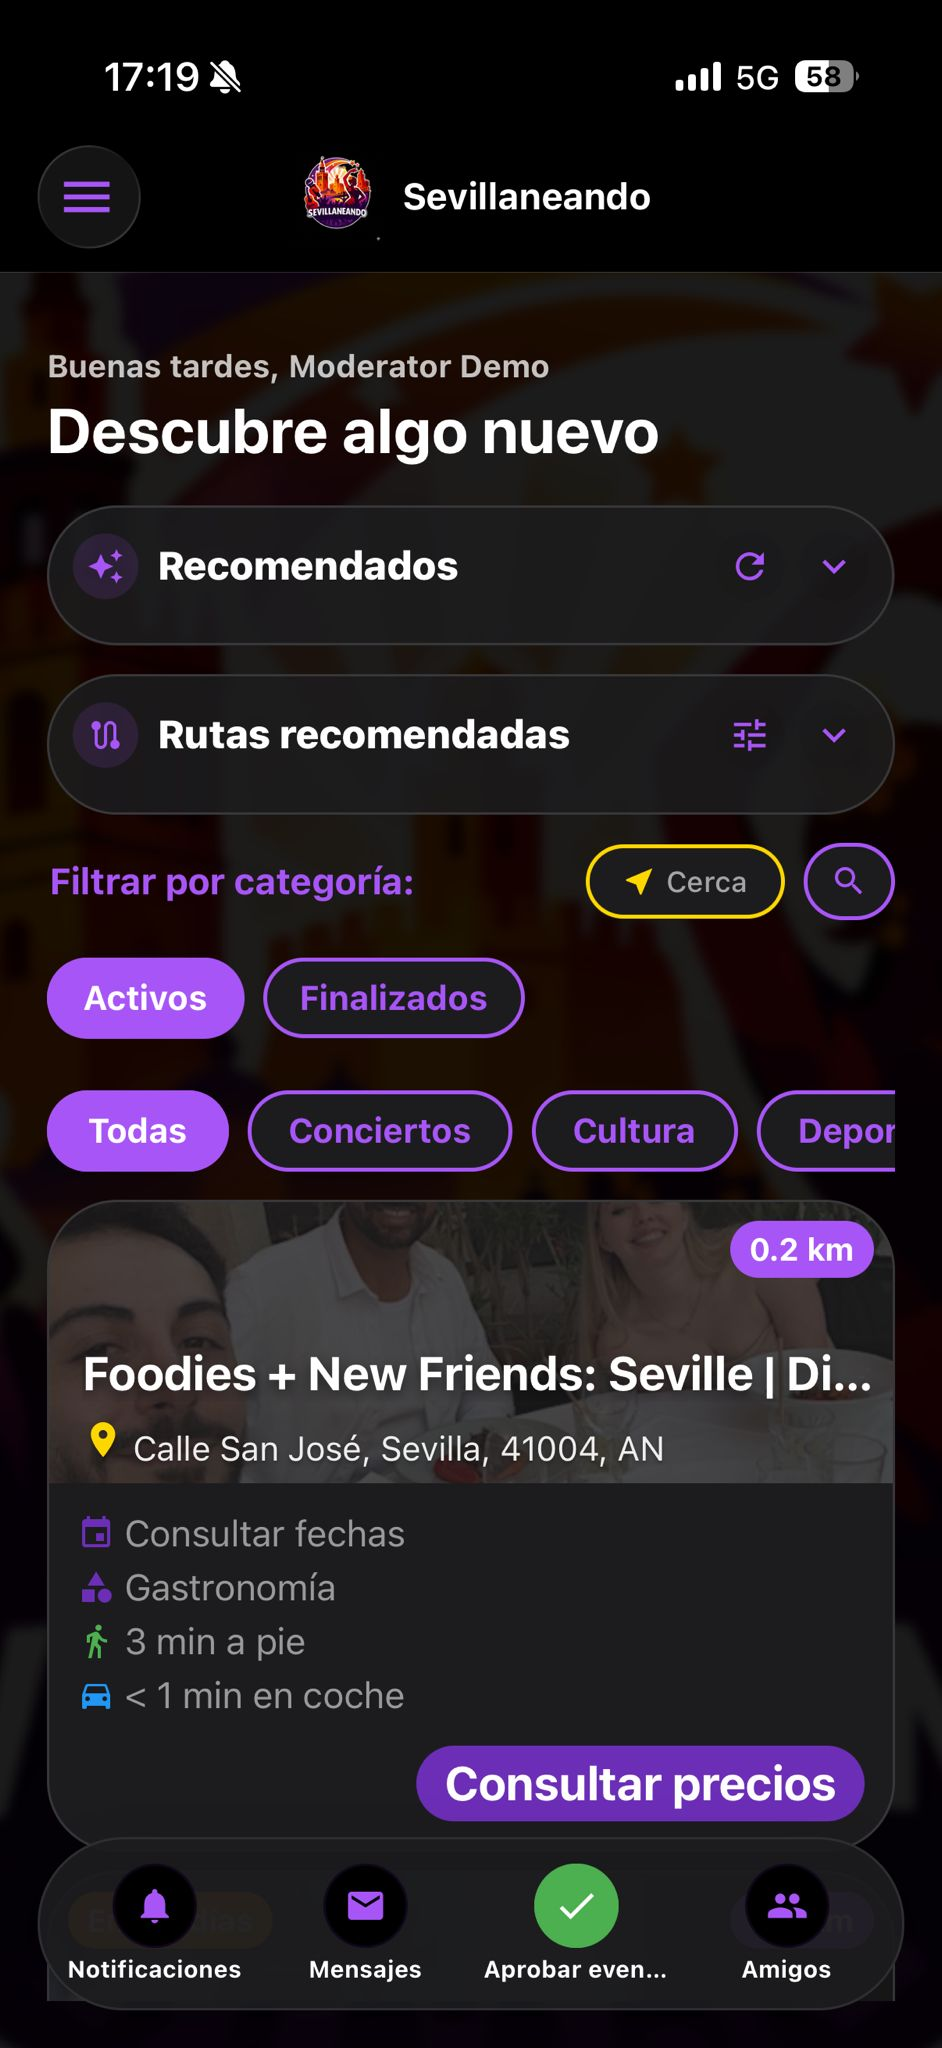
\includegraphics[width=\linewidth]{figures/paso14/pagina_principal.png}
        \caption{Página principal}
    \end{subfigure}
    \hspace{0.01\linewidth}
    \begin{subfigure}{0.31\linewidth}
        \centering
        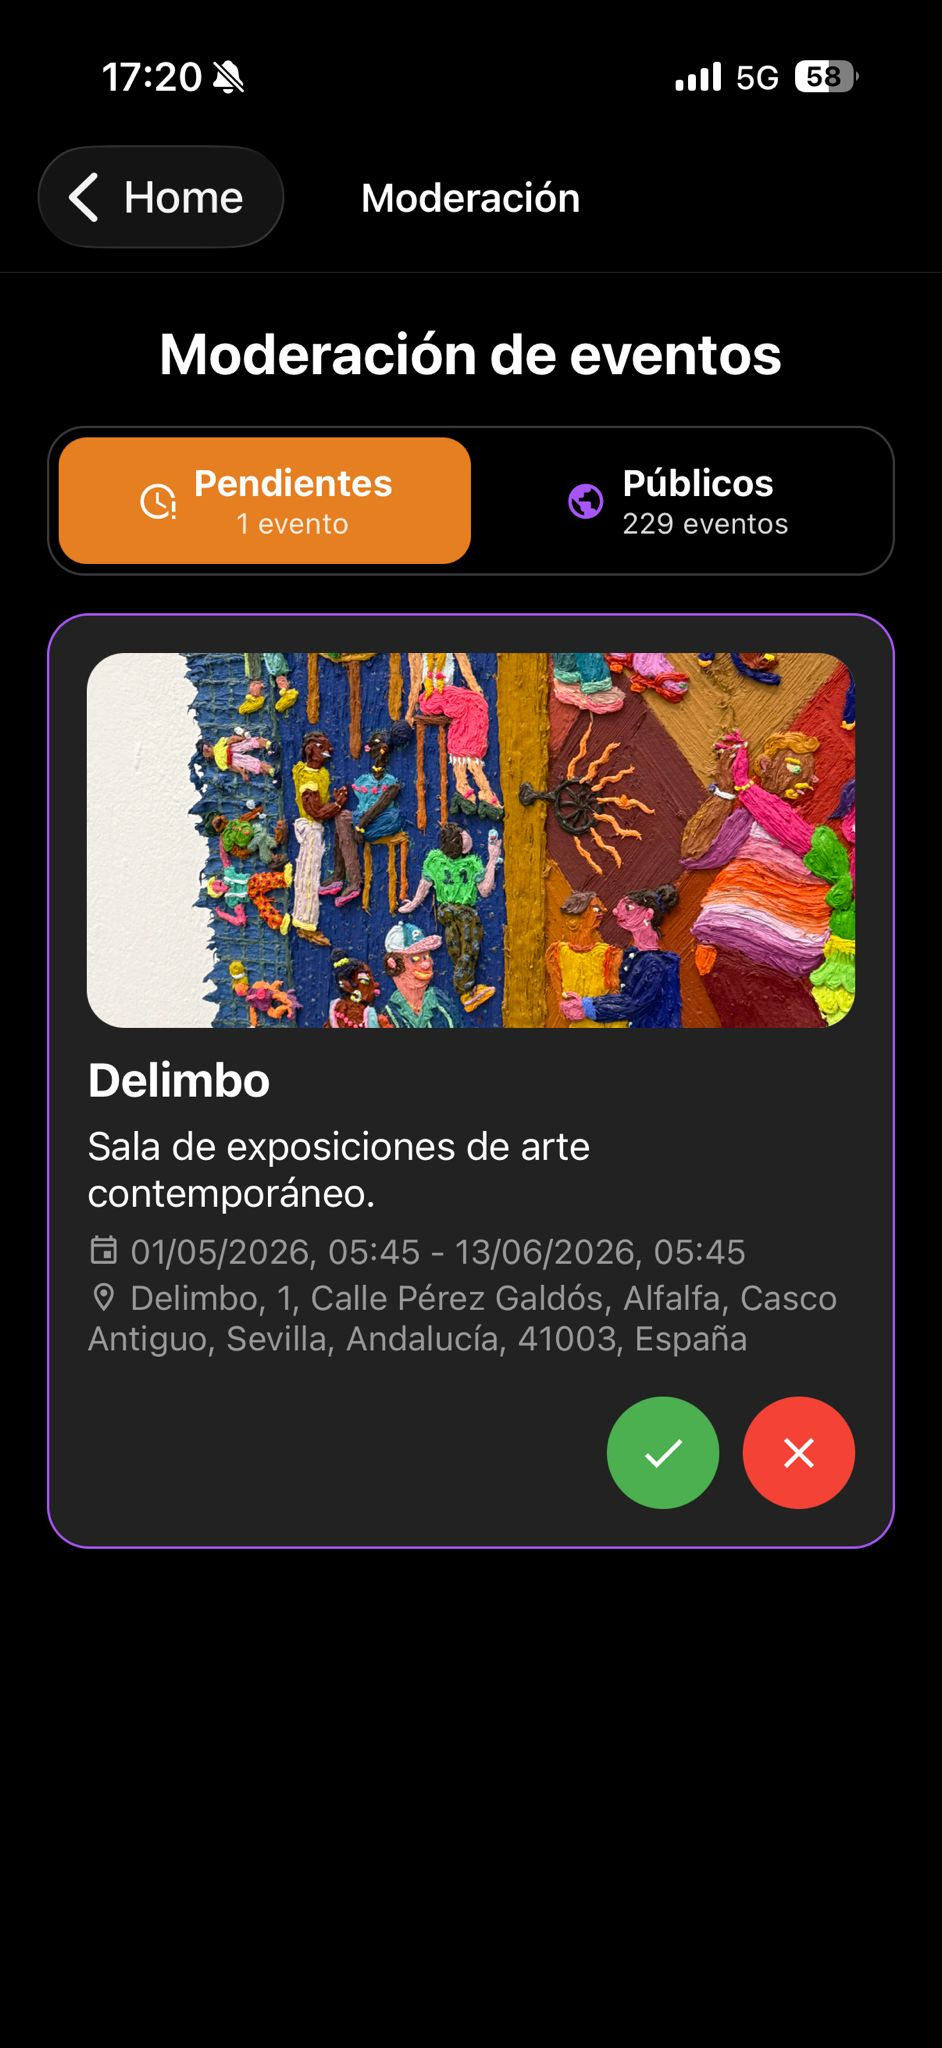
\includegraphics[width=\linewidth]{figures/paso14/moderacion.png}
        \caption{Moderación}
    \end{subfigure}
    \hspace{0.01\linewidth}
    \begin{subfigure}{0.31\linewidth}
        \centering
        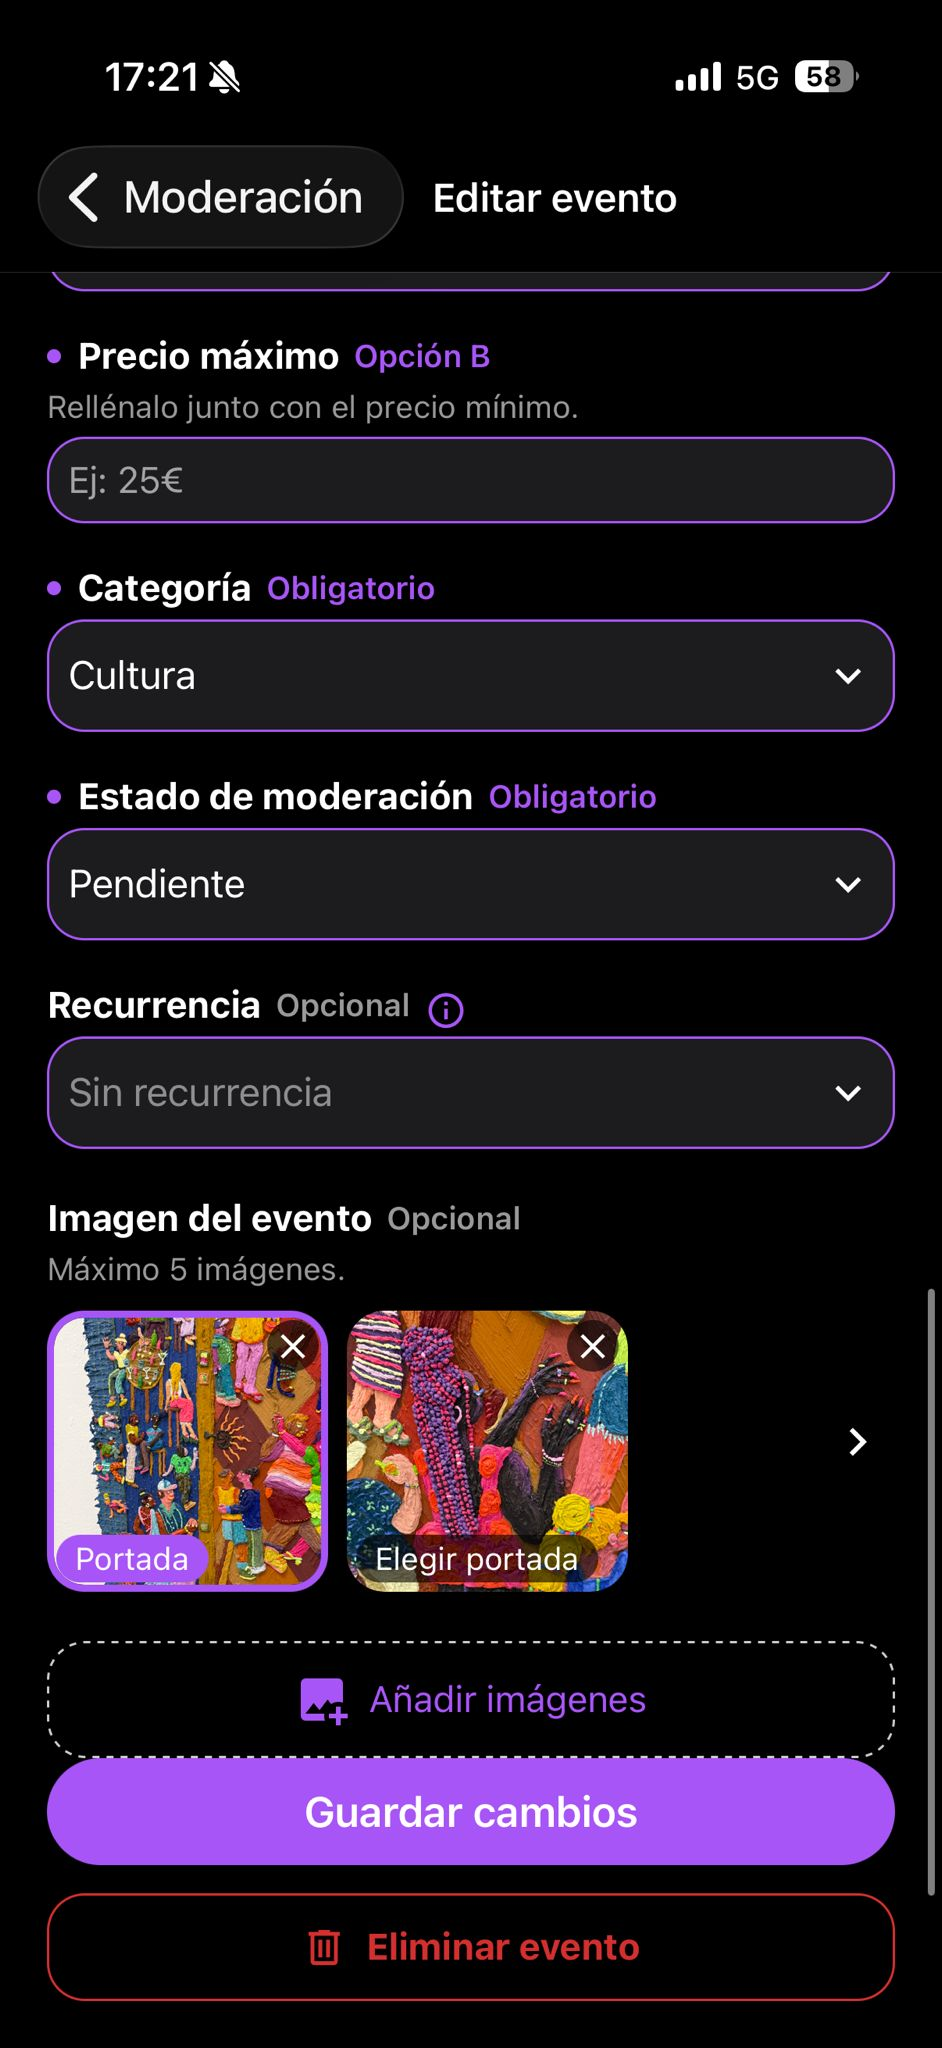
\includegraphics[width=\linewidth]{figures/paso14/editar_evento.png}
        \caption{Editar evento}
    \end{subfigure}
    \caption{Moderación de eventos}
\end{figure}

\clearpage

\subsection{Notificaciones (todos los roles)}

El acceso a las notificaciones se realiza desde el icono de campana situado en la barra inferior de la página principal, que muestra un indicador numérico con el total de notificaciones aún no leídas. Al pulsarlo se abre la pantalla \textit{Notificaciones}, donde aparecen listadas en orden cronológico inverso. Las notificaciones pueden referirse a la aprobación o el rechazo de un evento creado por el usuario, recordatorios previos a la celebración de eventos a los que está apuntado, avisos sobre eventos cercanos según su ubicación o nuevos seguidores.

Cada notificación incluye un icono representativo del tipo, un mensaje descriptivo y la fecha. Las notificaciones aún no leídas se distinguen visualmente del resto. Al pulsar una notificación esta queda marcada automáticamente como leída y, en función de su contenido, la aplicación abre el destino asociado: las notificaciones de seguidores llevan al perfil público de la persona que ha empezado a seguir al usuario, y las notificaciones relacionadas con un evento abren su pantalla de detalle. En la cabecera de la pantalla se incluye también un botón para marcar todas las notificaciones como leídas de una sola vez, lo que actualiza el indicador de la página principal sin necesidad de abrir cada una. Las notificaciones pueden eliminarse individualmente mediante el botón correspondiente que aparece en cada elemento.

\begin{figure}[H]
    \centering
    \begin{subfigure}{0.4\linewidth}
        \centering
        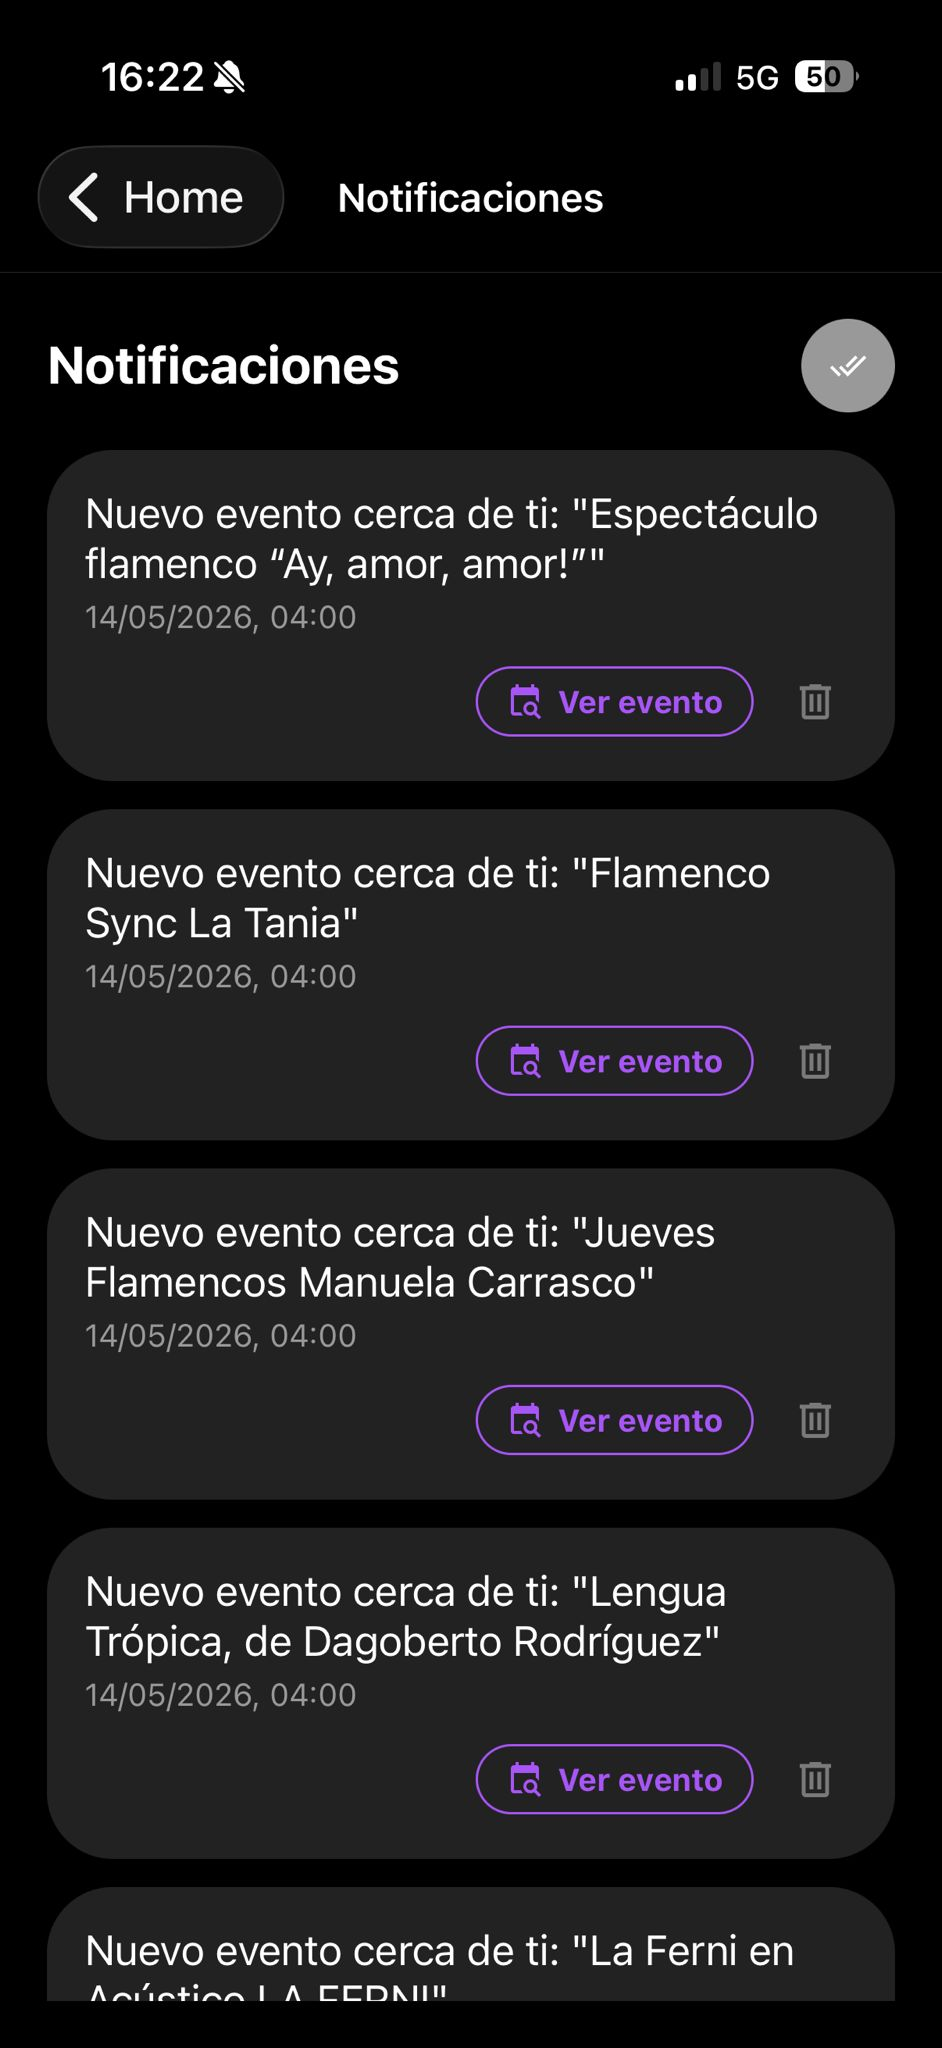
\includegraphics[width=\linewidth]{figures/paso15/notificaciones.png}
    \end{subfigure}
    \caption{Notificaciones}
\end{figure}

\clearpage

\subsection{Amistad y mensajería privada (todos los roles)}

La aplicación incorpora un módulo social que combina relaciones de amistad con mensajería privada. Para acceder se pulsa el icono de amigos en la barra inferior de la página principal, lo que abre una pantalla con cuatro pestañas en la cabecera. La pestaña \textit{Seguidores} muestra todas las personas que siguen al usuario; la pestaña \textit{Seguidos} muestra las personas a las que el usuario sigue; la pestaña \textit{Amigos} reúne las relaciones mutuas, es decir, los usuarios que se siguen entre sí; y la pestaña \textit{Buscar} incluye un campo de texto para localizar nuevos perfiles por nombre.

En cualquiera de los listados, cada elemento muestra el avatar y el nombre del usuario. Al pulsar sobre un usuario se abre su perfil público, donde se muestran sus datos básicos, el número de seguidores y seguidos, los eventos a los que asiste y los botones de acción. El botón \textit{Seguir} (o \textit{Dejar de seguir} si ya existe la relación) cambia su estado al pulsarlo. El botón de mensaje inicia una conversación privada en la pantalla \textit{Chat directo}. Los contadores de seguidores y seguidos del perfil son pulsables: al tocarlos se abre una pantalla independiente con la lista completa correspondiente a ese usuario, lo que permite descubrir nuevos perfiles a través de las conexiones de los demás.

La mensajería privada puede iniciarse también desde el chat de un evento, manteniendo pulsado un mensaje ajeno o pulsando el icono de sobre que aparece junto al mensaje, así como desde la lista de asistentes de un evento. En la pantalla de chat directo se pueden enviar mensajes de texto e imágenes mediante los iconos de galería y cámara situados junto al campo de escritura. Al pulsar sobre una imagen recibida se abre a pantalla completa con posibilidad de ampliarla con dos dedos. Manteniendo pulsado un mensaje propio aparece la opción de eliminarlo.

Todas las conversaciones privadas se conservan y son accesibles posteriormente desde el icono de mensajes de la barra inferior de la página principal. La pantalla \textit{Mensajes} lista las conversaciones existentes con la última actividad de cada una, y al pulsar sobre una se reanuda el chat con todo el historial.

\begin{figure}[H]
    \centering
    \begin{subfigure}{0.305\linewidth}
        \centering
        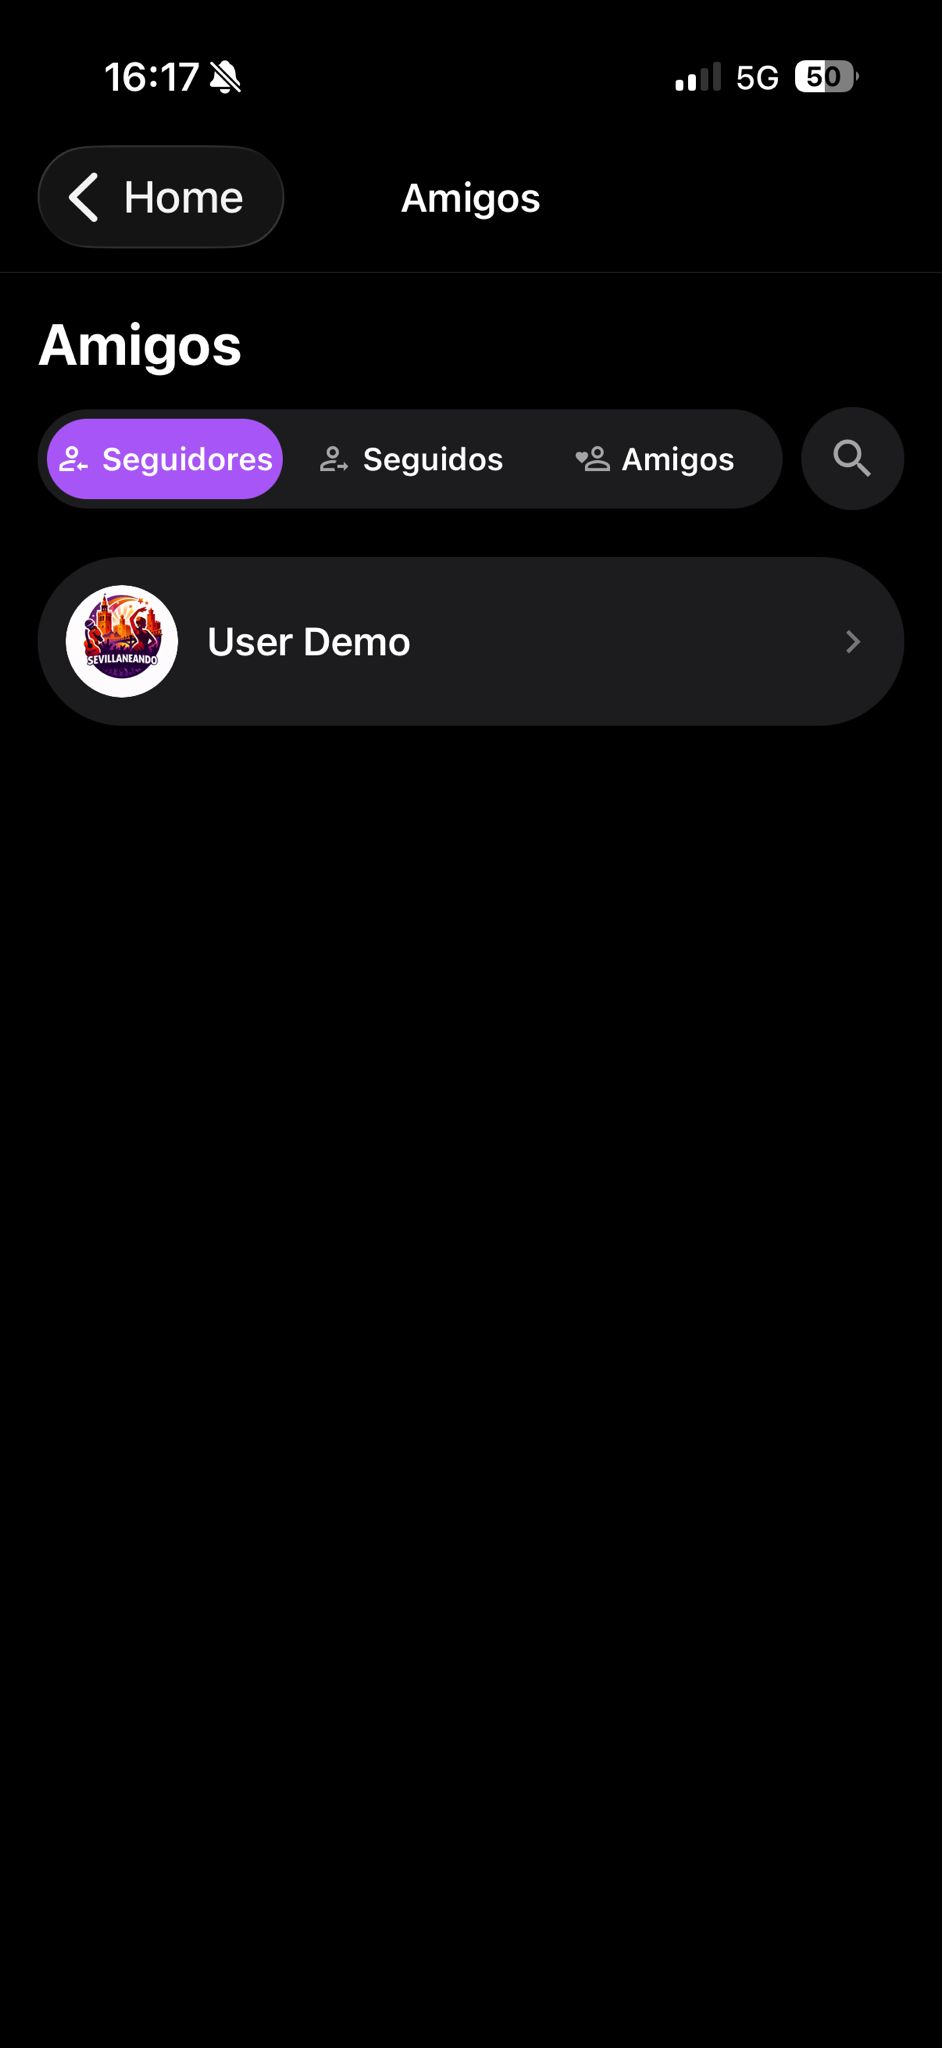
\includegraphics[width=\linewidth]{figures/paso16/amistad.png}
        \caption{Módulo de amistad}
    \end{subfigure}
    \hspace{0.02\linewidth}
    \begin{subfigure}{0.31\linewidth}
        \centering
        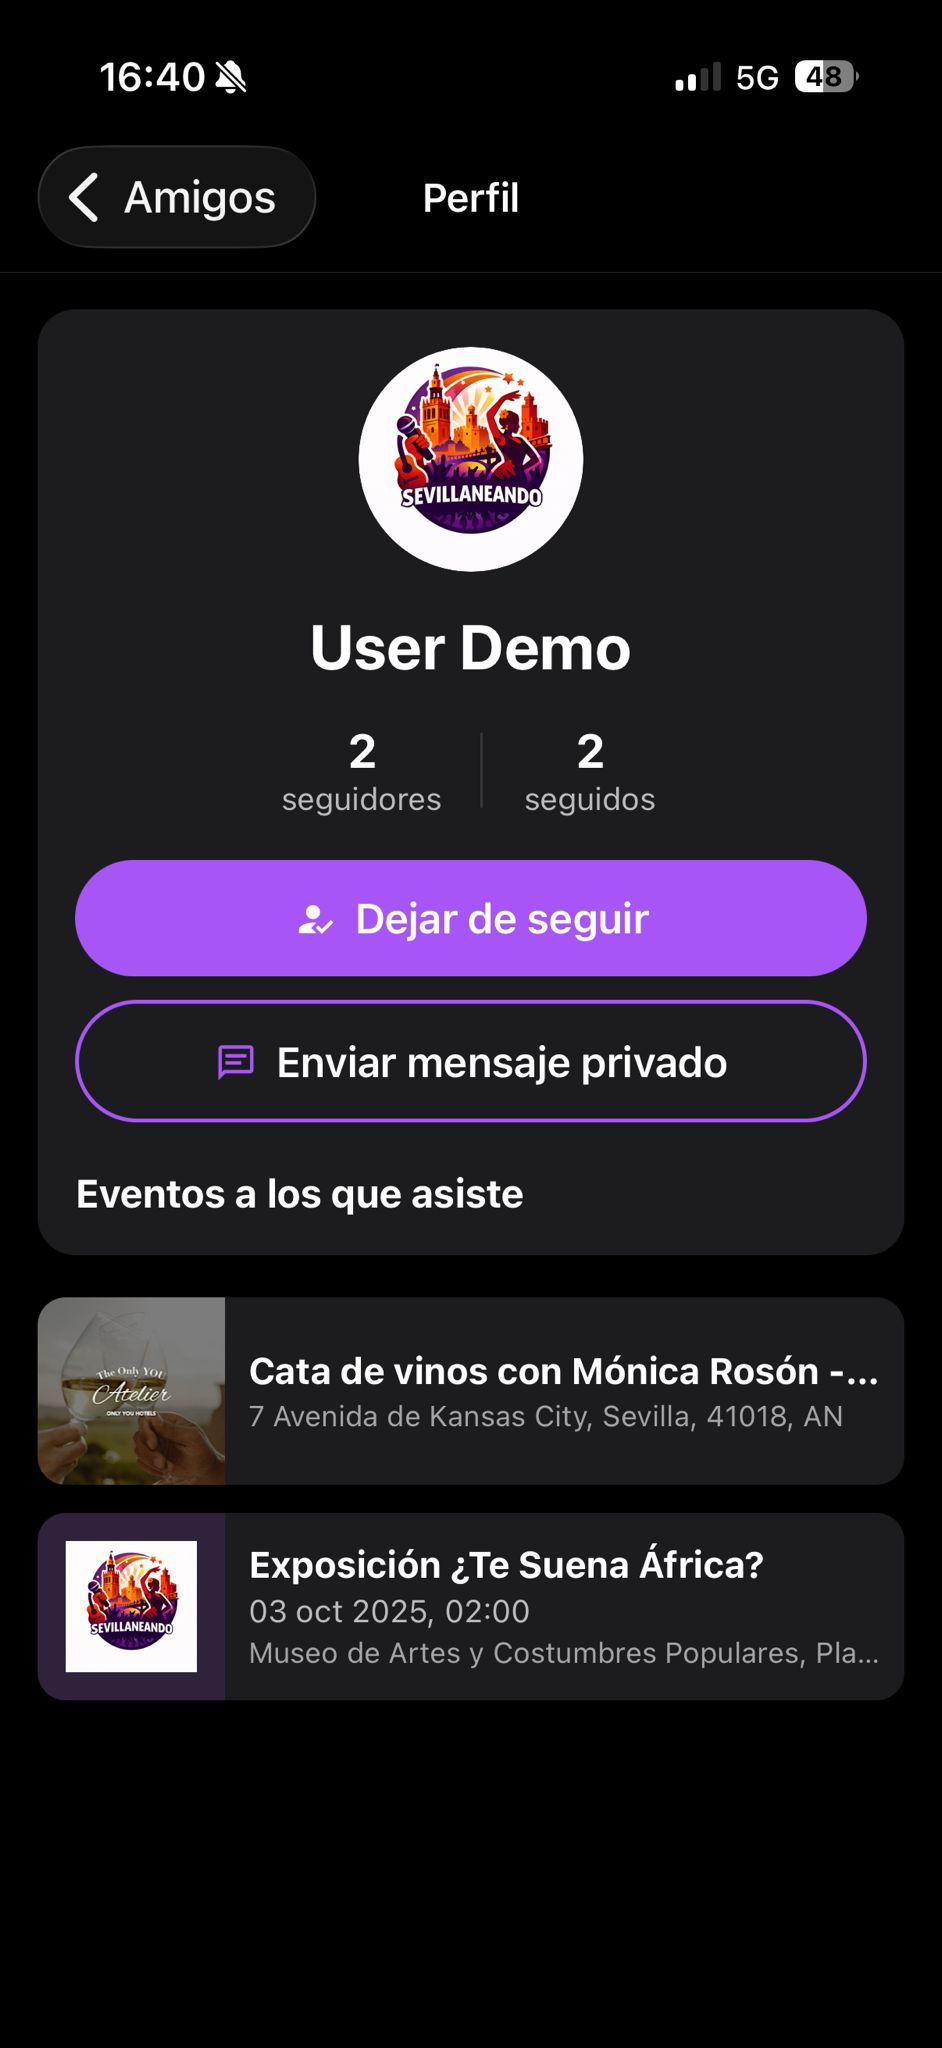
\includegraphics[width=\linewidth]{figures/paso16/ver_perfil.png}
        \caption{Ver perfil}
    \end{subfigure}
    \caption{Amistad y perfil de usuario}
\end{figure}

\begin{figure}[H]
    \centering
    \begin{subfigure}{0.305\linewidth}
        \centering
        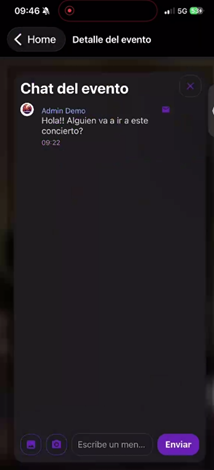
\includegraphics[width=\linewidth]{figures/paso16/chat_evento.png}
        \caption{Chat del evento}
    \end{subfigure}
    \hspace{0.02\linewidth}
    \begin{subfigure}{0.31\linewidth}
        \centering
        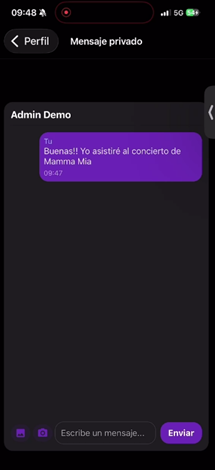
\includegraphics[width=\linewidth]{figures/paso16/chat_priv.png}
        \caption{Chat privado}
    \end{subfigure}
    \caption{Mensajes privados}
\end{figure}

\begin{figure}[H]
    \centering
    \begin{subfigure}{0.358\linewidth}
        \centering
        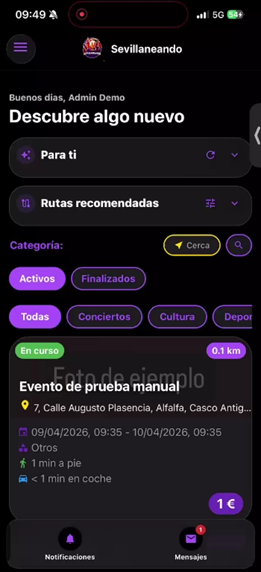
\includegraphics[width=\linewidth]{figures/paso16/pag_ppal.png}
        \caption{Página principal}
    \end{subfigure}
    \hspace{0.02\linewidth}
    \begin{subfigure}{0.373\linewidth}
        \centering
        
\includegraphics[width=\linewidth]{figures/paso16/mensajes.png}
        \caption{Mensajes}
    \end{subfigure}
    \caption{Consulta de mensajes privados}
\end{figure}

\clearpage

\subsection{Eventos finalizados}

Los eventos cuyo intervalo de fechas ya ha pasado se consideran finalizados y la aplicación los trata de forma diferenciada. En la página principal aparecen únicamente al activar la pestaña \textit{Eventos finalizados}, situada junto a \textit{Eventos activos}, y siguen siendo accesibles desde los listados personales del usuario (guardados, apuntados o creados) en los que ya estuvieran presentes.

Al abrir el detalle de un evento finalizado, la información se muestra con normalidad pero el botón principal del panel de acciones aparece deshabilitado con la etiqueta \textit{Finalizado}, impidiendo nuevas inscripciones. El usuario que ya estaba apuntado mantiene su asistencia registrada en el historial. El resto de acciones siguen activas en la medida en que tienen sentido: pueden consultarse los asistentes, abrir la ubicación en mapas externos, leer las opiniones y dejar una valoración del evento. Esta distinción permite preservar la utilidad informativa del sistema sin confundir al usuario sobre la disponibilidad real de cada actividad.

\begin{figure}[H]
    \centering
    \begin{subfigure}{0.4\linewidth}
        \centering
        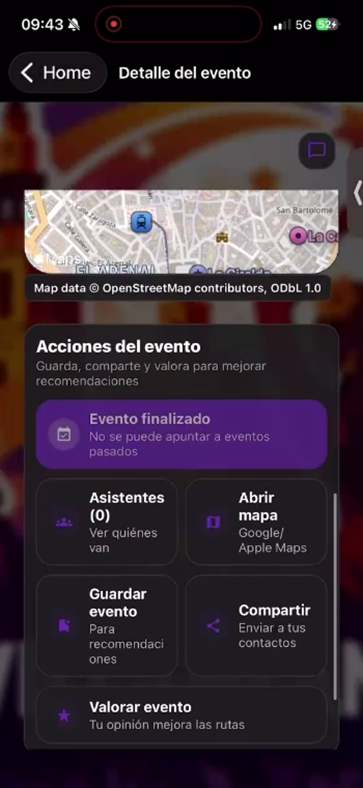
\includegraphics[width=\linewidth]{figures/paso17/evento_fin.png}
    \end{subfigure}
    \caption{Evento finalizado}
\end{figure}

\clearpage

\subsection{Guía de uso integrada}

La aplicación incorpora una guía de uso accesible directamente desde el menú lateral, en el apartado \textit{Información} → \textit{Guía de uso}. Esta guía está pensada para resolver dudas frecuentes sin necesidad de consultar documentación externa.

La guía se presenta en formato de acordeón: cada sección puede desplegarse de forma independiente para mostrar su contenido. Las secciones disponibles son las siguientes:

\begin{itemize}[leftmargin=1.5em]
    \item \textbf{Crear un evento.} Explica el proceso de creación de eventos, incluyendo los campos obligatorios y opcionales.
    \item \textbf{Precio de un evento.} Aclara las opciones de precio disponibles: gratuito, precio fijo o rango de precios.
    \item \textbf{Recurrencia.} Describe cómo crear eventos que se repiten periódicamente.
    \item \textbf{Eventos privados y enlace de acceso.} Explica qué es un evento privado, cómo se comparte mediante enlace y que no pasa por moderación.
    \item \textbf{Moderación de eventos.} Informa sobre el proceso de revisión de los eventos públicos antes de su publicación.
    \item \textbf{Guardar eventos.} Detalla cómo guardar eventos de interés para consultarlos más adelante.
    \item \textbf{Apuntarse a un evento.} Describe el proceso de inscripción a un evento y dónde encontrar los eventos a los que el usuario está apuntado.
    \item \textbf{Calendario de eventos.} Explica la vista de calendario y cómo navegar entre fechas.
    \item \textbf{Mapa de eventos.} Indica cómo funciona el mapa y la importancia de tener la ubicación del perfil configurada.
    \item \textbf{Categorías.} Explica para qué sirven las categorías y cómo pueden reorganizarse.
    \item \textbf{Rutas recomendadas.} Describe la funcionalidad de rutas que agrupa eventos cercanos entre sí.
    \item \textbf{Perfil e intereses.} Explica cómo configurar el perfil y los intereses, que influyen en las recomendaciones.
    \item \textbf{Amigos y seguidores.} Detalla las relaciones sociales disponibles en la aplicación.
    \item \textbf{Valorar un evento.} Informa sobre cómo dejar una reseña o valoración una vez finalizado el evento.
    \item \textbf{Chat del evento.} Explica el chat grupal asociado a cada evento y las condiciones de acceso.
\end{itemize}

\begin{figure}[H]
    \centering
    \begin{subfigure}{0.4\linewidth}
        \centering
        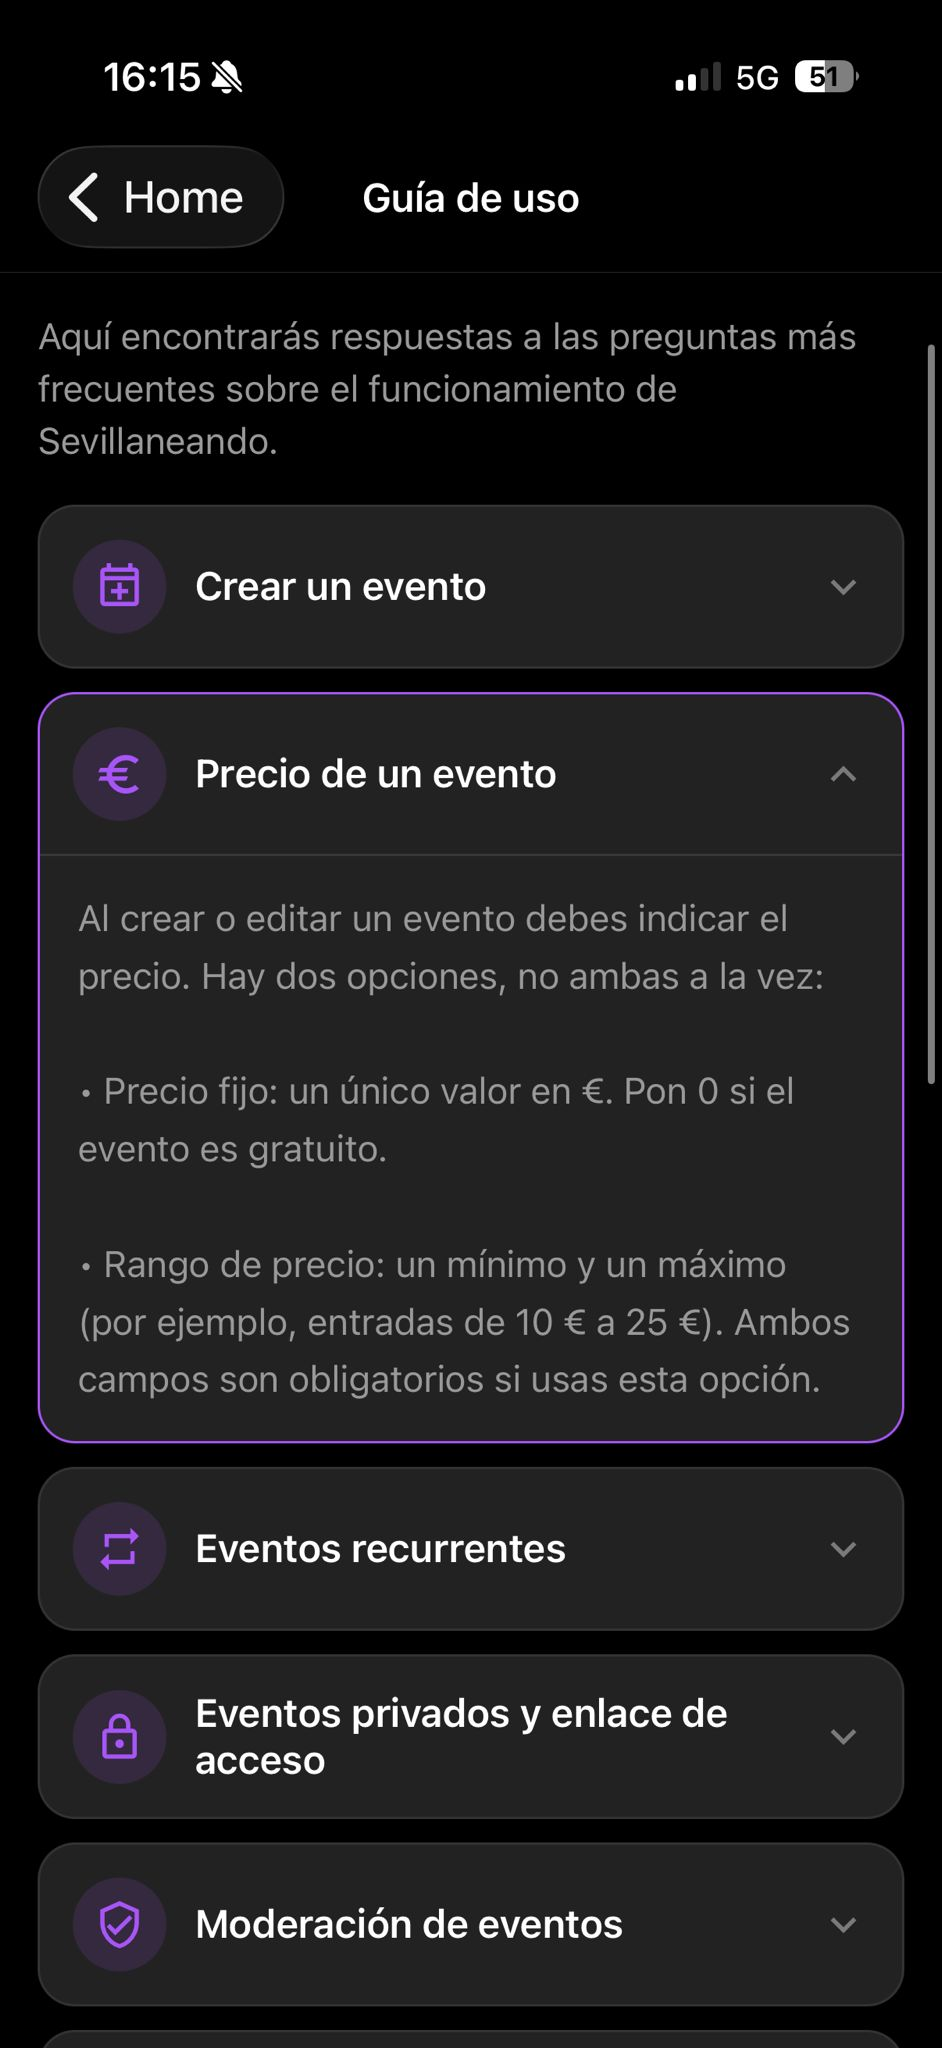
\includegraphics[width=\linewidth]{figures/paso18/guia_uso.png}
    \end{subfigure}
    \caption{Guía de uso integrada en la aplicación}
\end{figure}

\clearpage

\section{Grafo de navegabilidad}

Con el fin de complementar la guía de uso, se recomienda incluir un grafo de navegabilidad que muestre las principales pantallas de la aplicación y las rutas de transición más habituales entre ellas. Este diagrama ayuda a comprender la estructura general del sistema y la manera en que el usuario se desplaza por sus distintos módulos.

\begin{figure}[H]
    \centering
    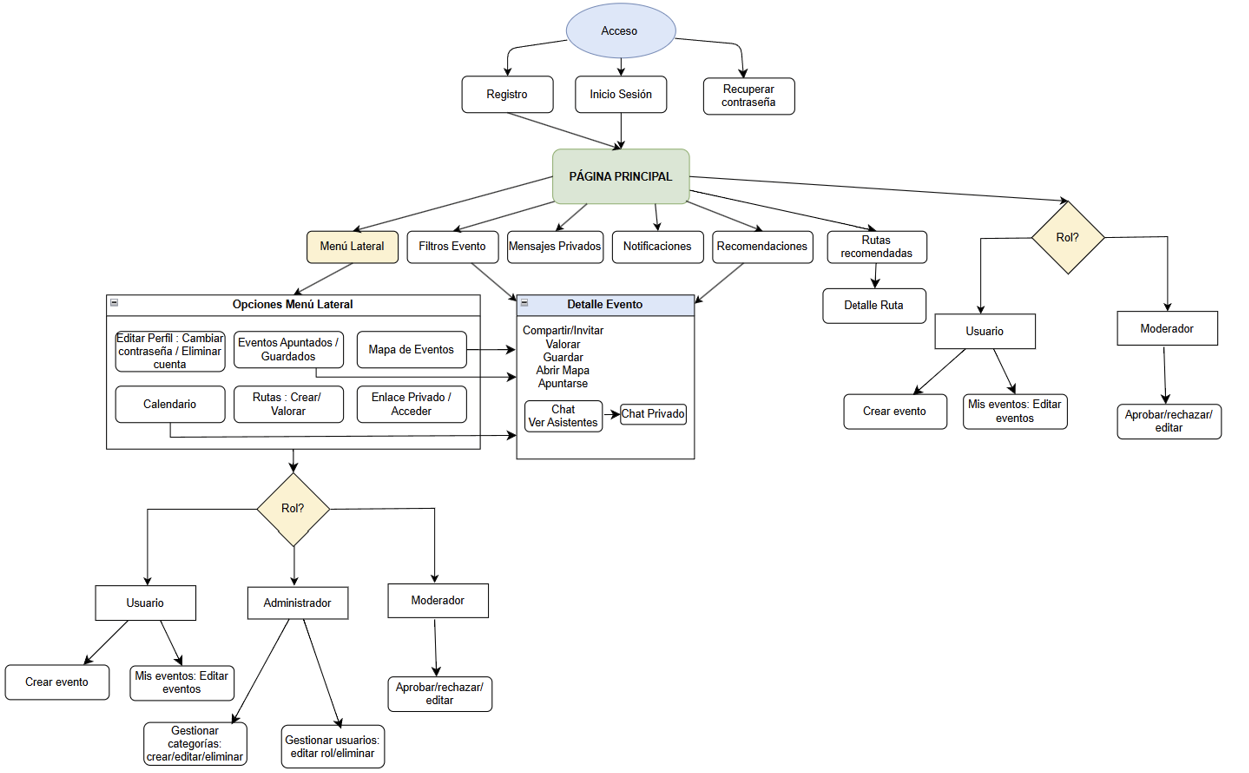
\includegraphics[width=\linewidth,height=0.99\textheight,keepaspectratio]{figures/grafo_navegacion.png}
    \caption{Grafo de navegabilidad de la aplicación}
\end{figure}

\section{Errores frecuentes}

A continuación se recogen algunos problemas habituales que pueden producirse durante el uso de la aplicación, junto con una posible explicación:

\begin{itemize}[leftmargin=1.5em]
\item \textbf{No aparecen eventos en el mapa.} Puede deberse a que el usuario no ha definido una ubicación en el perfil.
\item \textbf{No llegan notificaciones de eventos cercanos.} Puede ser necesario revisar los permisos de ubicación.
\item \textbf{No es posible apuntarse a un evento.} Es posible que el evento se encuentre finalizado o no admita nuevas inscripciones.
\item \textbf{No se puede compartir un evento privado libremente.} En este tipo de eventos la capacidad de invitación queda restringida al creador.
\item \textbf{Las recomendaciones no resultan relevantes.} El sistema mejora sus propuestas a medida que el usuario interactúa con la aplicación.
\item \textbf{No se visualizan correctamente algunas funciones basadas en proximidad.} Debe comprobarse que la ubicación del perfil está configurada correctamente.
\end{itemize}
